\documentclass[11pt]{book}
\usepackage{notes}

%%%%%%%%%%%%%%%%%%%%%%%%%%%%%%%%%%%%%%%%%%%%%%%%%%

\begin{document}

\frontmatter

\begin{titlepage}
\phantom{.} \vspace{0.5in} \\
{\Huge \bf MATH 307} \vspace{1mm} \\
{\it Applied Linear Algebra}
\begin{center}
\includegraphics[width=6.5in]{cover.png}
\end{center}
\flushright{\it \today \ \ v0.1}
\end{titlepage}

\thispagestyle{empty}
\setcounter{page}{0}
\tableofcontents

%%%%%%%%%%%%%%%%%%%%%%%%%%%%%%%%%%%%%%%%%%%%%%%%%%

\chapter{Preface}
\section*{Learning Goals}

\begin{itemize}[leftmargin=*]
\item Summarize properties and constructions of matrix decompositions LU, QR and SVD
\item Perform matrix computations using mathematical software Python, SciPy and Jupyter
\item Compute solutions of large systems of linear equations using matrix decompositions
\item Compute least squares approximations of large linear systems using matrix decompositions
\item Compute eigenvalues of large matrices using iterative methods
\item Analyze digital signals using the discrete Fourier transform
\item Create and analyze mathematical models of real-world phenomenon
\end{itemize}

\section*{Prerequisites}

We assume the reader has completed an introductory undergraduate course in linear algebra:
\begin{itemize}[leftmargin=*]
\item linear systems of equations, row operations, elementary matrices and Gaussian elimination
\item linear independence, span, subspaces, dimension and rank
\item linear transformations, null space, row space and and column space of a matrix
\item matrix multiplication, inverses and determinants
\item eigenvalues and eigenvectors, characteristic polynomial and diagonalization
\item dot product, length, orthogonality, orthogonal projection and Gram–Schmidt orthogonalization
\end{itemize} 
See \href{https://courses.students.ubc.ca/cs/courseschedule?pname=subjarea&tname=subj-course&dept=MATH&course=221}{MATH 221}, \href{https://courses.students.ubc.ca/cs/courseschedule?pname=subjarea&tname=subj-course&dept=MATH&course=223}{MATH 223} and \href{https://courses.students.ubc.ca/cs/courseschedule?pname=subjarea&tname=subj-course&dept=MATH&course=152}{MATH 152} at \href{https://www.math.ubc.ca}{UBC Math}.

\section*{Under Construction}

This is a work in progress and the following sections are still under construction:

\begin{itemize}
\item Computed Tomography
\item Eigenvalue Problems: Exercises on pseudoinverse, SVD expansion, image deblurring, computed tomography 
\item Convolution Theorem and Filtering
\end{itemize}

%%%%%%%%%%%%%%%%%%%%%%%%%%%%%%%%%%%%%%%%%%%%%%%%%%

\mainmatter

\chapter{Linear Systems of Equations} \newpage
\section{Review: Linear Systems}

\begin{bigidea}
Solve a linear system of equations $A \bs{x} = \bs{b}$ by reducing the augmented matrix $[ \, A \ \bs{b} \, ]$ to row-echelon form via Gaussian elimination.
\end{bigidea}

\begin{definition}
A {\bf linear system of equations} \cite[p.1]{KN} is a collection of equations of the form
$$
\begin{array}{ccccccccc}
a_{1,1} x_1 & + & a_{1,2} x_2 & + & \cdots & + & a_{1,n} x_n & = & b_1 \\
a_{2,1} x_1 & + & a_{2,2} x_2 & + & \cdots & + & a_{2,n} x_n & = & b_2 \\
& & & & & & & \vdots & \\
a_{m,1} x_1 & + & a_{m,2} x_2 & + & \cdots & + & a_{m,n} x_n & = & b_m
\end{array}
$$
where the coefficients $a_{i,j}$, $b_i$ are known constants. In matrix notation, we have $A \bs{x} = \bs{b}$ where
$$
A = 
\begin{bmatrix}
a_{1,1} & a_{1,2} & \cdots & a_{1,n} \\
a_{2,1} & a_{2,2} & \cdots & a_{2,n} \\
\vdots & \vdots & \ddots & \vdots \\
a_{m,1} & a_{m,2} & \cdots & a_{m,n}
\end{bmatrix}
\hspace{10mm}
\bs{x} = \begin{bmatrix} x_1 \\ x_2 \\ \vdots \\ x_n \end{bmatrix}
\hspace{10mm}
\bs{b} = \begin{bmatrix} b_1 \\ b_2 \\ \vdots \\ b_m \end{bmatrix}
$$
\end{definition}

\begin{definition}
The following are called {\bf elementary row operations} \cite[p.5]{KN}:
\begin{enumerate}
\item Interchange two rows.
\item Multiply one row by a nonzero number.
\item Add a multiple of one row to a different row.
\end{enumerate}
\end{definition}

\begin{definition}
A matrix is in {\bf row-echelon form} \cite[p.10]{KN} if:
\begin{enumerate}
\item All zero rows are at the bottom.
\item The first nonzero entry in a row (from the left) is 1.
\item The first nonzero entry in a row (from the left) is located to the right of the first nonzero entry in every row above.
\end{enumerate}
For example:
$$
\begin{bmatrix} 1 & * & * \\ 0 & 1 & * \\ 0 & 0 & 1 \end{bmatrix} \hspace{5mm}
\begin{bmatrix} 1 & * & * & * & * \\ 0 & 1 & * & * & * \\ 0 & 0 & 1 & * & * \\ 0 & 0 & 0 & 0 & 0 \end{bmatrix} \hspace{5mm}
\begin{bmatrix} 1 & * & * & * & * \\ 0 & 0 & 1 & * & * \\ 0 & 0 & 0 & 0 & 1 \\ 0 & 0 & 0 & 0 & 0 \end{bmatrix} \hspace{5mm}
\begin{bmatrix}  1 & * \\ 0 & 0 \end{bmatrix}
$$
\end{definition}

\begin{theorem}
Every matrix can be transformed to row-echelon form by a sequence of elementary row operations via the Gaussian elimination algorithm \cite[p.11]{KN}.
\end{theorem}

\begin{example}
Find all solutions of $A \bs{x} = \bs{b}$ for:
\begin{enumerate}
\item $A = \begin{bmatrix} 1 & 1 & 1 \\ 1 & 0 & 1 \\ 2 & 5 & 2 \end{bmatrix}$ \hspace{3mm} $\bs{b} = \begin{bmatrix} 2 \\ 1 \\ 7 \end{bmatrix}$
\item $A = \left[ \begin{array}{rrrr} 1 & -1 & \phantom{+}1 & -2 \\ -1 & 1 & 1 & 1 \\ -1 & 2 & 3 & 1 \\ 1 & -1 & 2 & 1 \end{array} \right]$ \hspace{3mm} $\bs{b} = \left[ \begin{array}{r} 1 \\ -1 \\ 2 \\ 1 \end{array} \right]$
\item $A = \begin{bmatrix} 1 & 1 & 2 & 1 \\ 1 & 0 & 1 & 1 \\ 0 & 1 & 1 & 0 \end{bmatrix}$ \hspace{3mm} $\bs{b} = \begin{bmatrix} 1 \\ 1 \\ 2 \end{bmatrix}$
\end{enumerate}
Implement Gaussian elimination for each example:
\begin{enumerate}
\item $\left[ \begin{array}{rrr|r} 1 & 1 & 1 & 2 \\ 1 & 0 & 1 & 1 \\ 2 & 5 & 2 & 7 \end{array} \right] \ \longrightarrow \ \left[ \begin{array}{rrr|r} 1 & 1 & 1 & 2 \\ 0 & 1 & 0 & 1 \\ 0 & 0 & 0 & 0 \end{array} \right] \Rightarrow \ \ \bs{x} = \begin{bmatrix} 1-t \\ 1 \\ t \end{bmatrix} \ , \ \ t \in \mathbb{R}$
\item $\left[ \begin{array}{rrrr|r} 1 & -1 & \phantom{+}1 & -2 & 1 \\ -1 & 1 & 1 & 1 & -1 \\ -1 & 2 & 3 & 1 & 2 \\ 1 & -1 & 2 & 1 & 1 \end{array} \right] \longrightarrow \left[ \begin{array}{rrrr|r} 1 & -1 & \phantom{+}1 & -2 & \phantom{+}1 \\ 0 & 1 & 4 & -1 & 3 \\ 0 & 0 & 1 & 3 & 0 \\ 0 & 0 & 0 & 1 & 0 \end{array} \right]  \Rightarrow \ \ \bs{x} = \begin{bmatrix} 4 \\ 3 \\ 0 \\ 0 \end{bmatrix}$
\item $\left[ \begin{array}{rrrr|r} 1 & 1 & 2 & 1 & 1 \\ 1 & 0 & 1 & 1 & 1 \\ 0 & 1 & 1 & 0 & 2 \end{array} \right] \longrightarrow \left[ \begin{array}{rrrr|r} 1 & 1 & 2 & 1 & 1 \\ 0 & 1 & 1 & 0 & 0 \\ 0 & 0 & 0 & 0 & 1 \end{array} \right] \ \Rightarrow \ \ $ No solution
\end{enumerate}
\end{example}

\begin{definition}
The {\bf rank} of a matrix $A$ \cite[p.16]{KN} is the number of nonzero rows in the row-echelon form of $A$.
\end{definition}

\begin{example} Let $A$ be $m \times n$ matrix with $\mathrm{rank}(A) = r$. Describe when the linear system $A \bs{x} = \bs{b}$ has: a unique solution, infinitely many solutions, or no solutions. \\

The system $A \bs{x} = \bs{b}$ is inconsistent (ie.~no solution) if $\mathrm{rank}(A) < \mathrm{rank}([ \, A \ \bs{b} \, ])$. That is, the row-echelon form of the augmented matrix $[ \, A \ \bs{b} \, ]$ has a row of the form
$$
\begin{array}{rrrr|r} 0 & 0 & \cdots & 0 & 1 \end{array}
$$
which implies $0 = 1$. The system has a unique solution when $\mathrm{rank}(A) = \mathrm{rank}([ \, A \ \bs{b} \, ])$ and $\mathrm{rank}(A) = n$. That is, the rank is equal to the number of variables in the system. Finally, the system has infinitely many solutions when $\mathrm{rank}(A) = \mathrm{rank}([ \, A \ \bs{b} \, ])$ and $\mathrm{rank}(A) < n$.
\end{example}
\section{LU and Cholesky Decompositions}

\begin{bigidea}
The LU decomposition of a matrix $A$ (if it exists) records the row operations of Gaussian elimination in a matrix factorization $A=LU$ where $L$ is a unit lower triangular matrix and $U$ is an upper triangular matrix. If $A$ is symmetric positive definite, then the Cholesky decomposition $A = LL^T$ always exists where $L$ is a lower triangular matrix (not unit lower in general).
\end{bigidea}

\begin{definition}
An {\bf elementary matrix} \cite[p.95]{KN} is a matrix $E$ obtained from the identity matrix $I$ by an elementary row operation. There are 3 types:
\begin{enumerate}
\item Switch rows $i$ and $j$. For example:
$$
\begin{bmatrix} 1 & 0 & 0 \\ 0 & 0 & 1 \\ 0 & 1 & 0 \end{bmatrix} \hspace{5mm}
\begin{bmatrix} 0 & 0 & 1 \\ 0 & 1 & 0 \\ 1 & 0 & 0 \end{bmatrix} \hspace{5mm}
\begin{bmatrix} 1 & 0 & 0 & 0 \\ 0 & 0 & 0 & 1 \\ 0 & 0 & 1 & 0 \\ 0 & 1 & 0 & 0 \end{bmatrix} \hspace{5mm}
\begin{bmatrix} 0 & 0 & 0 & 0 & 1 \\ 0 & 1 & 0 & 0 & 0 \\ 0 & 0 & 1 & 0 & 0 \\ 0 & 0 & 0 & 1 & 0 \\ 1 & 0 & 0 & 0 & 0 \end{bmatrix}
$$
\item Multiply row $i$ by $c$. For example:
$$
\begin{bmatrix} 1 & 0 & 0 \\ 0 & 2 & 0 \\ 0 & 0 & 1 \end{bmatrix} \hspace{5mm}
\begin{bmatrix} 1 & 0 & 0 & 0 \\ 0 & 1 & 0 & 0 \\ 0 & 0 & 3 & 0 \\ 0 & 0 & 0 & 1 \end{bmatrix} \hspace{5mm}
\left[ \begin{array}{rrrrr} 1 & \phantom{+}0 & \phantom{+}0 & \phantom{+}0 & \phantom{+}0 \\
0 & -5 & 0 & 0 & 0 \\ 0 & 0 & 1 & 0 & 0 \\ 0 & 0 & 0 & 1 & 0 \\ 0 & 0 & 0 & 0 & 1 \end{array} \right]
$$
\item Add $c$ times row $i$ to row $j$. For example:
$$
\begin{bmatrix} 1 & 0 & 0 \\ 0 & 1 & 0 \\ 4 & 0 & 1 \end{bmatrix} \hspace{5mm}
\begin{bmatrix} 1 & 0 & 0 & 0 \\ 0 & 1 & 0 & 0 \\ 0 & 8 & 1 & 0 \\ 0 & 0 & 0 & 1 \end{bmatrix} \hspace{5mm}
\left[ \begin{array}{rrrrr} 1 & \phantom{+}0 & \phantom{+}0 & \phantom{+}0 & \phantom{+}0 \\
0 & 1 & 0 & 0 & 0 \\ 0 & 0 & 1 & 0 & 0 \\ 0 & 0 & 0 & 1 & 0 \\ 0 & 0 & -2 & 0 & 1 \end{array} \right]
$$
\end{enumerate}
\end{definition}

\begin{proposition}
Let $E$ be an elementary matrix. Then matrix multiplication $EA$ applies the corresponding row operation to $A$ \cite[p.96]{KN}.
\end{proposition}

\begin{definition}
A {\bf unit lower triangular matrix} (see \href{https://en.wikipedia.org/wiki/Triangular_matrix}{Wikipedia: Triangular matrix}) is a square matrix with ones on the diagonal and zeros above diagonal. For example:
$$
\begin{bmatrix} 1 & & \\ * & 1 & & \\ * & * & 1 & \\ * & * & * & 1 \end{bmatrix}
$$
An {\bf atomic lower triangular matrix} has nonzero entries below the diagonal in only one column:
$$
L_k =
\begin{bmatrix}
1 & & & & & \\
 & \ddots & & & & \\
 & & 1 & & & \\
 & & \ell_{k+1,k}& 1 & & \\
 & & \vdots & & \ddots & \\
 & & \ell_{m,k} & & & 1 \\
\end{bmatrix}
$$
\end{definition}

\begin{proposition}
\begin{enumerate}
\item Let $A$ be a $m$ by $n$ matrix and let $L_k$ be an atomic lower triangular matrix with nonzero entries in column $k$. Multiplication $L_k A$ adds $\ell_{i,k}$ times row $k$ of $A$ to row $i$ for each $i = k+1,\dots,m$.
\item The inverse of an atomic lower triangular matrix:
$$
L_k =
\begin{bmatrix}
1 & & & & & \\
 & \ddots & & & & \\
 & & 1 & & & \\
 & & \ell_{k+1,k}& 1 & & \\
 & & \vdots & & \ddots & \\
 & & \ell_{m,k} & & & 1 \\
\end{bmatrix}
\hspace{5mm} \Rightarrow \hspace{5mm} 
L_k^{-1} =
\begin{bmatrix}
1 & & & & & \\
 & \ddots & & & & \\
 & & 1 & & & \\
 & & -\ell_{k+1,k}& 1 & & \\
 & & \vdots & & \ddots & \\
 & & -\ell_{m,k} & & & 1 \\
\end{bmatrix}
$$
\item Multiplication of atomic lower triangular matrices:
\begin{align*}
L_1 L_2 \cdots L_{m-1} &=
\begin{bmatrix}
1 & & & & \\
\ell_{2,1} & 1 & & & \\
\ell_{3,1} & & 1 & & \\
\vdots & & & \ddots & \\
\ell_{m,1} & & & & 1 \\
\end{bmatrix}
\begin{bmatrix}
1 & & & & \\
& 1 & & & \\
& \ell_{3,2} & 1 & & \\
& \vdots & & \ddots & \\
& \ell_{m,2} & & & 1 \\
\end{bmatrix}
\dots
\begin{bmatrix}
1 & & & & \\
& 1 & & & \\
& & 1 & & \\
& & & \ddots & \\
& & & \ell_{m,m-1} & 1 \\
\end{bmatrix} \\
&=
\begin{bmatrix}
1 & & & & \\
\ell_{2,1} & 1 & & & \\
\ell_{3,1} & \ell_{3,2} & 1 & & \\
\vdots & \vdots & \ddots & \ddots & \\
\ell_{m,1} & \ell_{m,2} & \cdots & \ell_{m,m-1} & 1 \\
\end{bmatrix}
\end{align*}
\end{enumerate}
\end{proposition}

\begin{theorem}
If $A$ can be reduced by Gaussian elimination to row echelon form without pivoting (that is, without interchanging rows), then
$$A = LU$$
where $L$ is a unit lower triangular matrix and $U$ is an upper triangular matrix. This is called the {\bf LU decomposition} of $A$ \cite[p.68]{MH}. The algorithm is:
\begin{enumerate}
\item[] Let $m$ be the number of rows of $A$ and let $n$ be the number of columns.
\item[] Let $A_1 = A$ and use notation $A_k = \left[ a_{i,j}^{(k)} \right]$.
\item[] {\bf for} $k$ from 1 to $n-1$:
\begin{enumerate}
\item[] Let $L_k$ such that $\ds \ell_{i,k} = - \frac{a^{(k)}_{i,k}}{a^{(k)}_{k,k}}$ and compute $L_k A_k = A_{k+1}$.
\end{enumerate}
\item[] {\bf end}
\item[] $A = LU$ where $L = L_1^{-1} \cdots L_{n-1}^{-1}$ is unit lower triangular and $U = A_n$ is upper triangular
\end{enumerate}
\end{theorem}

\begin{note}
In each step of the LU decomposition algorithm, the operation $L_k A_k$ eliminates entries in $A_k$ below the diagonal in column $k$. The result is $L_{n-1} \cdots L_1 A = U$ where $U = A_n$ is upper triangular and therefore $A = LU$ where $L = L_1^{-1} \cdots L_{n-1}^{-1}$ is unit lower triangular.
\end{note}

\begin{example}
Compute the LU decomposition of
$$
A = \begin{bmatrix} 2 & 1 & 1 \\ 2 & 0 & 2 \\ 4 & 3 & 4 \end{bmatrix}
$$
Start with $A_1 = A$ and compute
\begin{align*}
L_1 A_1 &= \begin{bmatrix} \phantom{-}1 & 0 & 0 \\ -1 & 1 & 0 \\ -2 & 0 & 1 \end{bmatrix}
\begin{bmatrix} 2 & 1 & 1 \\ 2 & 0 & 2 \\ 4 & 3 & 4 \end{bmatrix}
=
\left[ \begin{array}{rrr} 2 & 1 & 1 \\ 0 & -1 & \phantom{+}1 \\ 0 & 1 & 2 \end{array} \right] \\
L_2 A_2 &= \begin{bmatrix} 1 & 0 & 0 \\ 0 & 1 & 0 \\ 0 & 1 & 1 \end{bmatrix}
\left[ \begin{array}{rrr} 2 & 1 & 1 \\ 0 & -1 & \phantom{+}1 \\ 0 & 1 & 2 \end{array} \right]
=
\left[ \begin{array}{rrr} 2 & 1 & 1 \\ 0 & -1 & \phantom{+}1 \\ 0 & 0 & 3 \end{array} \right]
\end{align*}
Therefore $A = LU$ where
$$
L = L_1^{-1} L_2^{-1}
%= \begin{bmatrix} 1 & 0 & 0 \\ 1 & 1 & 0 \\ 2 & 0 & 1 \end{bmatrix}
%\left[ \begin{array}{rrr}  1 & 0 & 0 \\ 0 & 1 & 0 \\ 0 & -1 & \phantom{+}1 \end{array} \right]
=
\left[ \begin{array}{rrr} 1 & 0 & 0 \\ 1 & 1 & 0 \\ 2 & -1 & \phantom{+}1 \end{array} \right]
\hspace{10mm}
U = \left[ \begin{array}{rrr} 2 & 1 & 1 \\ 0 & -1 & \phantom{+}1 \\ 0 & 0 & 3 \end{array} \right] \\
$$
\end{example}

\begin{note} Suppose $A$ has an LU decomposition $A = LU$. Applications of LU are:
\begin{enumerate}
\item Solve the system of equations $A \bs{x} = \bs{b}$ by:
\begin{itemize}
\item Solve $L \bs{y} = \bs{b}$ by forward substitution
\item Solve $U \bs{x} = \bs{y}$ by backward substitution
\end{itemize} 
\item $\mathrm{rank}(A) = \mathrm{rank}(U)$
\item $\det(A) = \det(U) =$ product of diagonal entries of $U$
\item Compute $A^{-1}$: use LU decomposition to solve $A \bs{x}_1 = \bs{e}_1, \dots, A \bs{x}_n = \bs{e}_n$ where $\bs{e}_k$ is the $k$th column of the identity $I$ and then $A^{-1} = [\bs{x}_1 \cdots \bs{x}_n]$ (that is, the columns of $A^{-1}$ are given by $\bs{x}_1, \dots, \bs{x}_n$)
\end{enumerate}
\end{note}

\begin{example}
Compute the LU decomposition of
$$
A = \left[ \begin{array}{rrrr} 1 & 0 & 2 & 1 \\ 2 & 1 & 5 & 3 \\ 1 & 0 & 0 & 2 \\ 0 & -1 & \phantom{+}1 & \phantom{+}1 \end{array} \right]
$$
Start with $A_1 = A$ and compute
\begin{align*}
L_1 A_1 &=
\left[ \begin{array}{rrrr} \phantom{+}1 & \phantom{+}0 & \phantom{+}0 & \phantom{+}0 \\ -2 & 1 & 0 & 0 \\ -1 & 0 & 1 & 0 \\ 0 & 0 & 0 & 1 \end{array} \right]
\left[ \begin{array}{rrrr} 1 & 0 & 2 & 1 \\ 2 & 1 & 5 & 3 \\ 1 & 0 & 0 & 2 \\ 0 & -1 & \phantom{+}1 & \phantom{+}1 \end{array} \right]
=
\left[ \begin{array}{rrrr} 1 & 0 & 2 & 1 \\ 0 & 1 & 1 & 1 \\ 0 & 0 & -2 & 1 \\ 0 & -1 & 1 & \phantom{+}1 \end{array} \right] \\
L_2 A_2 &=
\left[ \begin{array}{rrrr} \phantom{+}1 & \phantom{+}0 & \phantom{+}0 & \phantom{+}0 \\ 0 & 1 & 0 & 0 \\ 0 & 0 & 1 & 0 \\ 0 & 1 & 0 & 1 \end{array} \right]
\left[ \begin{array}{rrrr} 1 & 0 & 2 & 1 \\ 0 & 1 & 1 & 1 \\ 0 & 0 & -2 & 1 \\ 0 & -1 & 1 & \phantom{+}1 \end{array} \right]
=
\left[ \begin{array}{rrrr} 1 & 0 & 2 & 1 \\ 0 & 1 & 1 & 1 \\ 0 & 0 & -2 & 1 \\ 0 & \phantom{+}0 & 2 & \phantom{+}2 \end{array} \right] \\
L_3 A_3 &=
\left[ \begin{array}{rrrr} \phantom{+}1 & \phantom{+}0 & \phantom{+}0 & \phantom{+}0 \\ 0 & 1 & 0 & 0 \\ 0 & 0 & 1 & 0 \\ 0 & 0 & 1 & 1 \end{array} \right]
\left[ \begin{array}{rrrr} 1 & 0 & 2 & 1 \\ 0 & 1 & 1 & 1 \\ 0 & 0 & -2 & 1 \\ 0 & \phantom{+}0 & 2 & \phantom{+}2 \end{array} \right]
=
\left[ \begin{array}{rrrr} 1 & 0 & 2 & 1 \\ 0 & 1 & 1 & 1 \\ 0 & 0 & -2 & 1 \\ 0 & \phantom{+}0 & 0 & \phantom{+}3 \end{array} \right]
\end{align*}
And we compute $A = LU$ using properties of atomic lower triangular matrices
$$
L
=
L_1^{-1} L_2^{-1} L_3^{-1}
=
%\left[ \begin{array}{rrrr} 1 & \phantom{+}0 & \phantom{+}0 & \phantom{+}0 \\ 2 & 1 & 0 & 0 \\ 1 & 0 & 1 & 0 \\ 0 & 0 & 0 & 1 \end{array} \right]
%\left[ \begin{array}{rrrr} 1 & \phantom{+}0 & \phantom{+}0 & \phantom{+}0 \\ 0 & 1 & 0 & 0 \\ 0 & 0 & 1 & 0 \\ 0 & -1 & 0 & 1 \end{array} \right]
%\left[ \begin{array}{rrrr} 1 & \phantom{+}0 & \phantom{+}0 & \phantom{+}0 \\ 0 & 1 & 0 & 0 \\ 0 & 0 & 1 & 0 \\ 0 & 0 & -1 & 1 \end{array} \right] \\
%=
\left[ \begin{array}{rrrr} 1 & 0 & 0 & 0 \\ 2 & 1 & 0 & 0 \\ 1 & 0 & 1 & 0 \\ 0 & -1 & -1 & \phantom{+}1 \end{array} \right]
\hspace{10mm}
U = \left[ \begin{array}{rrrr} 1 & 0 & 2 & 1 \\ 0 & 1 & 1 & 1 \\ 0 & 0 & -2 & 1 \\ 0 & \phantom{+}0 & 0 & \phantom{+}3 \end{array} \right]
$$
\end{example}

\begin{theorem}
Let $A$ be an $m$ by $n$ matrix. If $\mathrm{rank}(A) = m$ and $A$ has a LU decomposition $A = LU$ where $L$ is unit lower triangular and $U$ is upper triangular, then the matrices $L$ and $U$ are unique \cite[p.124]{KN}.
\end{theorem}

\begin{definition}
Let $A$ be a square matrix.
\begin{enumerate}
\item $A$ is {\bf symmetric} if $A^T = A$.
\item $A$ is {\bf positive definite} if $\bs{x}^T A \bs{x} > 0$ for all $\bs{x} \not= 0$.
\end{enumerate}
See \cite[p.84]{MH}.
\end{definition}

\begin{example}
If $A$ is invertible, then both $AA^T$ and $A^TA$ are symmetric positive definite.
\end{example}

\begin{theorem}
Let $A$ be a symmetric positive definite matrix. There exists a lower triangular matrix $L$ with positive diagonal entries (not necessarily unit lower triangular) such that
$$
A = L L^T
$$
This is called the {\bf Cholesky decomposition} of $A$ \cite[p.84]{MH}.
\end{theorem}

\begin{proposition}
Let $A$ be a symmetric positive definite matrix. There exists a {\it unit} lower triangular matrix $L$ and a diagonal matrix $D$ with {\it positive} entries such that
$$
A = LDL^T
$$
Furthermore, let $\sqrt{D}$ be the diagonal matrix where the entries are the square roots of the entries in $D$ (that is, $\sqrt{D}^2 = D$). Then
$$
A = (L\sqrt{D})(\sqrt{D}L^T)
$$
is the Cholesky decomposition of $A$.
\end{proposition}

\begin{example}
Computing the Cholesky decomposition requires about half the computations of the LU factorization since we need only compute $L$ or $U$ by Gaussian elimination. Compute the Cholesky decomposition of $A$ where $A = M^TM$ for
$$
M =
\left[ \begin{array}{rrr} 1 & 1 & -1 \\ 0 & -1 & -1 \\ 1 & 1 & 1 \end{array} \right]
\ \ \Rightarrow \ \
A =
\left[ \begin{array}{rrr} 2 & 2 & 0 \\ 2 & 3 & 1 \\ 0 & 1 & 3 \end{array} \right]
$$
We know that $A$ is symmetric positive definite by construction and so we proceed by Gaussian elimination (without scaling or switching rows)
$$
\left[ \begin{array}{rrr} 2 & 2 & 0 \\ 2 & 3 & 1 \\ 0 & 1 & 3 \end{array} \right]
\rightarrow
\left[ \begin{array}{rrr} 2 & 2 & 0 \\ 0 & 1 & 1 \\ 0 & 1 & 3 \end{array} \right]
\rightarrow
\left[ \begin{array}{ccc} 2 & 2 & 0 \\ 0 & 1 & 1 \\ 0 & 0 & 2 \end{array} \right]
$$
Factor out the diagonal
$$
\left[ \begin{array}{ccc} 2 & 2 & 0 \\ 0 & 1 & 1 \\ 0 & 0 & 2 \end{array} \right]
=
\left[ \begin{array}{ccc} 2 & 0 & 0 \\ 0 & 1 & 0 \\ 0 & 0 & 2 \end{array} \right]
\left[ \begin{array}{ccc} 1 & 1 & 0 \\ 0 & 1 & 1 \\ 0 & 0 & 1 \end{array} \right]
$$
Therefore the Cholesky decomposition is $A = LL^T$ where
$$
L = 
\left[ \begin{array}{ccc} 1 & 0 & 0 \\ 1 & 1 & 0 \\ 0 & 1 & 1 \end{array} \right]
\left[ \begin{array}{ccc} \sqrt{2} & 0 & 0 \\ 0 & 1 & 0 \\ 0 & 0 & \sqrt{2} \end{array} \right]
=
\left[ \begin{array}{ccc} \sqrt{2} & 0 & 0 \\ \sqrt{2} & 1 & 0 \\ 0 & 1 & \sqrt{2} \end{array} \right]
$$
\end{example}
\section{LU Decomposition with Partial Pivoting}

\begin{bigidea}
For any matrix $A$, Gaussian elimination with partial pivoting computes a decomposition $A = PLU$ where $P$ is a permutation matrix, $L$ is unit lower triangular and $U$ is upper triangular.
\end{bigidea}

\begin{note}
At step $k$ in the LU decomposition in the previous section, we form the atomic lower triangular matrix $L_k$ with entries
$$
\ell_{i,k} = - \frac{a_{i,k}^{(k)}}{a_{k,k}^{(k)}}
$$
This is a problem if $a_{k,k}^{(k)}$ very small or zero! Therefore in general we need to use pivoting. In other words, we interchange rows as necessary at each step. This leads to
$$
L_{n-1}P_{n-1} \cdots L_2 P_2 L_1 P_1 A = U
\hspace{5mm}
\Rightarrow
\hspace{5mm}
A = P_1^{-1}L_1^{-1} P_2^{-1}L_2^{-1} \cdots P_{n-1}^{-1} L_{n-1}^{-1} U
$$
We need to figure out how to rearrange the matrices into the form $A = PLU$.
\end{note}

\begin{proposition}
Let $L_k$ be an atomic lower triangular matrix with nonzero entries below the diagonal in column $k$. Let $P$ be an elementary permutation matrix which switches rows $i$ and $j$ for $i>k$ and $j>k$. Then $P L_k P = \tilde{L}_k$ where $\tilde{L}_k$ is simply $L_k$ but with entries $\ell_{i,k}$ and $\ell_{j,k}$ switched.

\begin{proof}
Write 
$L_k$ in block form
$$
L_k =
\begin{bmatrix}
1 & & & & & \\
& \ddots & & & & \\
& & 1 & & & \\
& & \ell_{k+1,k}& 1 & & \\
& & \vdots & & \ddots & \\
& & \ell_{m,k} & & & 1 \\
\end{bmatrix}
=
\left[ \begin{array}{c|c} I_k & 0 \\ \hline L_* & I_{m-k} \end{array} \right]
\hspace{10mm}
L_* = \left[ \begin{array}{cccc}
0 & \cdots & 0 & \ell_{k+1,k} \\
\vdots & & \vdots & \vdots \\
0 & \cdots & 0 & \ell_{m,k}
\end{array} \right]
$$
where $I_k$ and $I_{m-k}$ are the identity matrices of size $k$ and $m-k$ respectively. Since $P$ be an elementary permutation matrix which switches rows $i$ and $j$ for $i>k$ and $j>k$, write in block form
$$
\left[ \begin{array}{c|c} I_k & 0 \\ \hline 0 & P_* \end{array} \right]
$$
Since $P$ is an elementary permutation matrix which only switches 2 rows, we have $P^2 = I_m$ and also $P_*^2 = I_{m-k}$. Finally, using block matrices, we compute
\begin{align*}
P L_k P
&=
\left[ \begin{array}{c|c} I_k & 0 \\ \hline 0 & P_* \end{array} \right]
\left[ \begin{array}{c|c} I_k & 0 \\ \hline L_* & I_{m-k} \end{array} \right]
\left[ \begin{array}{c|c} I_k & 0 \\ \hline 0 & P_* \end{array} \right] \\
&=
\left[ \begin{array}{c|c} I_k & 0 \\ \hline 0 & P_* \end{array} \right]
\left[ \begin{array}{c|c} I_k & 0 \\ \hline L_* & P_* \end{array} \right] \\
&=
\left[ \begin{array}{c|c} I_k & 0 \\ \hline P_*L_* & P_*^2 \end{array} \right] \\
&=
\left[ \begin{array}{c|c} I_k & 0 \\ \hline P_*L_* & I_{m-k} \end{array} \right]
\end{align*}
The result is $P L_k P = \tilde{L}_k$ where $\tilde{L}_k$ is simply $L_k$ but with $\ell_{i,k}$ and $\ell_{j,k}$ switched.
\end{proof}
\end{proposition}

\begin{example}
Consider the matrices
$$
P =
\begin{bmatrix}
1 & 0 & 0 & 0 \\
0 & 0 & 0 & 1 \\
0 & 0 & 1 & 0 \\
0 & 1 & 0 & 0
\end{bmatrix}
\hspace{10mm}
L =
\begin{bmatrix}
1 & 0 & 0 & 0 \\
a & 1 & 0 & 0 \\
b & 0 & 1 & 0 \\
c & 0 & 0 & 1
\end{bmatrix}
$$
Since $P$ switches rows 2 and 4, we find
$$
P L P = \begin{bmatrix}
1 & 0 & 0 & 0 \\
c & 1 & 0 & 0 \\
b & 0 & 1 & 0 \\
a & 0 & 0 & 1
\end{bmatrix}
$$
\end{example}

\begin{theorem}
For any matrix $A$, there exists a permutation matrix $P$, unit lower triangular matrix $L$ and upper triangular matrix $U$ such that
$$
A = PLU
$$
This is the {\bf LU decomposition with partial pivoting} \cite[p.72]{MH}. The algorithm is:
\begin{enumerate}
\item[] Let $m$ be the number of rows of $A$ and let $n$ be the number of columns.
\item[] Let $A_1 = A$ and use notation $A_k = \left[ a_{i,j}^{(k)} \right]$ and $\tilde{A}_k = \left[ \tilde{a}_{i,j}^{(k)} \right]$.
\item[] {\bf for} $k$ from 1 to $n-1$:
\begin{enumerate}
\item[] Find index $p$ with maximum value $\left| a_{p,k}^{(k)} \right|$ in column $k$ of $A_k$ below diagonal
\item[] (or if all entries in column $k$ below diagonal are zero, move to the next column).
\item[] Let $P_k$ such that $P_k A_k = \tilde{A}_k$ switches rows $p$ and $k$.
\item[] Let $L_k$ such that $\ds \ell_{i,k} = - \frac{\tilde{a}^{(k)}_{i,k}}{\tilde{a}^{(k)}_{k,k}}$ and compute $L_k \tilde{A}_k = A_{k+1}$.
\end{enumerate}
\item[] {\bf end}
\item[] $A = PLU$ where $P=P_1 \cdots P_{n-1}$, $U = A_n$ and $L = \tilde{L}_1^{-1} \cdots \tilde{L}_{n-1}^{-1}$ where each $\tilde{L}_k^{-1}$ is given by $L_k^{-1}$ with entries permuted in order by $P_{k'}$ for each $k' > k$.
\end{enumerate}
\end{theorem}

\begin{note}
Pivoting ensures all the entries of $L$ below the diagonal satisfy $| \ell_{i,j} | \leq 1$ ($i > j$).
\end{note}

\begin{example}
Compute the LU decomposition with partial pivoting of
$$
A = \begin{bmatrix} 1 & 1 & 1 \\ 1 & 1 & 2 \\ 0 & 1 & 1 \end{bmatrix}
$$
In the first column, we see the maximum value $| a_{i,1}|$ is 1 and we do not need to pivot therefore $P_1 = I$ and $\tilde{A}_1 = A_1 = A$. Compute:
$$
L_1 \tilde{A}_1 =
\left[ \begin{array}{rrr} 1 & 0 & 0 \\ -1 & 1 & 0 \\ 0 & 0 & 1 \end{array} \right]
\left[ \begin{array}{rrr} 1 & 1 & 1 \\ 1 & 1 & 2 \\ 0 & 1 & 1 \end{array} \right]
=
\left[ \begin{array}{rrr} 1 & 1 & 1 \\ 0 & 0 & 1 \\ 0 & 1 & 1 \end{array} \right]
$$
In the second column, we see $a_{2,2}^{(2)} = 0$ and $a_{3,2}^{(2)} = 1$ therefore we must swap rows
$$
P_2 A_2 = \left[ \begin{array}{rrr} 1 & 1 & 1 \\ 0 & 1 & 1 \\ 0 & 0 & 1 \end{array} \right]
$$
This is already upper triangular and so $L_2 = I$ in the last step. Therefore
$$
L_2 P_2 L_1 P_1 A = U \ \ \Rightarrow \ \ A = P_1^{-1} L_1^{-1} P_2^{-1}L_2^{-1} U = L_1^{-1} P_2^{-1} U
$$
Using the proposition above we find $ L_1^{-1} P_2^{-1} =   P_2^{-1} \tilde{L}_1^{-1}$ where
$$
\tilde{L}_1^{-1} = \left[ \begin{array}{rrr} 1 & 0 & 0 \\ 0 & 1 & 0 \\ 1 & 0 & 1 \end{array} \right]
$$
Finally, we have $A = PLU$ where
$$
P = \begin{bmatrix} 1 & 0 & 0 \\ 0 & 0 & 1 \\ 0 & 1 & 0 \end{bmatrix}
\hspace{5mm}
L = \begin{bmatrix} 1 & 0 & 0 \\ 0 & 1 & 0 \\ 1 & 0 & 1 \end{bmatrix}
\hspace{5mm}
U = \begin{bmatrix} 1 & 1 & 1 \\ 0 & 1 & 1 \\ 0 & 0 & 1 \end{bmatrix}
$$
\end{example}

\begin{example}
Suppose the LU decomposition with partial pivoting applied to $A$ yields matrices
$$
P_1 = \begin{bmatrix} 0 & 0 & 0 & 1 \\ 0 & 1 & 0 & 0 \\ 0 & 0 & 1 & 0 \\ 1 & 0 & 0 & 0 \end{bmatrix}
\hspace{5mm}
P_2 = \begin{bmatrix} 1 & 0 & 0 & 0 \\ 0 & 0 & 1 & 0 \\ 0 & 1 & 0 & 0 \\ 0 & 0 & 0 & 1 \end{bmatrix}
\hspace{5mm}
P_3 = \begin{bmatrix} 1 & 0 & 0 & 0 \\ 0 & 1 & 0 & 0 \\ 0 & 0 & 0 & 1 \\ 0 & 0 & 1 & 0 \end{bmatrix}
$$
$$
L_1 = \left[ \begin{array}{cccc} 1 & 0 & 0 & 0 \\ 0.2 & 1 & 0 & 0 \\ -0.1 & 0 & 1 & 0 \\ 0.5 & 0 & 0 & 1 \end{array} \right]
\hspace{5mm}
L_2 = \left[ \begin{array}{cccc} 1 & 0 & 0 & 0 \\ 0 & 1 & 0 & 0 \\ 0 & 0.7 & 1 & 0 \\ 0 & -0.1 & 0 & 1 \end{array} \right]
\hspace{5mm}
L_3 = \left[ \begin{array}{cccc} 1 & 0 & 0 & 0 \\ 0 & 1 & 0 & 0 \\ 0 & 0 & 1 & 0 \\ 0 & 0 & 0.1 & 1 \end{array} \right]
$$
We rearrange the matrices
\begin{align*}
& P_1^{-1} L_1^{-1} P_2^{-1} L_2^{-1} P_3^{-1} L_3^{-1} \\
&=
P_1
\left[ \begin{array}{cccc} 1 & 0 & 0 & 0 \\ -0.2 & 1 & 0 & 0 \\ 0.1 & 0 & 1 & 0 \\ -0.5 & 0 & 0 & 1 \end{array} \right]
P_2
\left[ \begin{array}{cccc} 1 & 0 & 0 & 0 \\ 0 & 1 & 0 & 0 \\ 0 & -0.7 & 1 & 0 \\ 0 & 0.1 & 0 & 1 \end{array} \right]
P_3
\left[ \begin{array}{cccc} 1 & 0 & 0 & 0 \\ 0 & 1 & 0 & 0 \\ 0 & 0 & 1 & 0 \\ 0 & 0 & -0.1 & 1 \end{array} \right] \\
&=
P_1 P_2
\left[ \begin{array}{cccc} 1 & 0 & 0 & 0 \\ 0.1 & 1 & 0 & 0 \\ -0.2 & 0 & 1 & 0 \\ -0.5 & 0 & 0 & 1 \end{array} \right]
P_3
\left[ \begin{array}{cccc} 1 & 0 & 0 & 0 \\ 0 & 1 & 0 & 0 \\ 0 & 0.1 & 1 & 0 \\ 0 & -0.7 & 0 & 1 \end{array} \right]
\left[ \begin{array}{cccc} 1 & 0 & 0 & 0 \\ 0 & 1 & 0 & 0 \\ 0 & 0 & 1 & 0 \\ 0 & 0 & -0.1 & 1 \end{array} \right] \\
&=
P_1 P_2 P_3
\left[ \begin{array}{cccc} 1 & 0 & 0 & 0 \\ 0.1 & 1 & 0 & 0 \\ -0.5 & 0 & 1 & 0 \\ -0.2 & 0 & 0 & 1 \end{array} \right]
\left[ \begin{array}{cccc} 1 & 0 & 0 & 0 \\ 0 & 1 & 0 & 0 \\ 0 & 0.1 & 1 & 0 \\ 0 & -0.7 & 0 & 1 \end{array} \right]
\left[ \begin{array}{cccc} 1 & 0 & 0 & 0 \\ 0 & 1 & 0 & 0 \\ 0 & 0 & 1 & 0 \\ 0 & 0 & -0.1 & 1 \end{array} \right] \\
&=
P_1 P_2 P_3
\left[ \begin{array}{cccc} 1 & 0 & 0 & 0 \\ 0.1 & 1 & 0 & 0 \\ -0.5 & 0.1 & 1 & 0 \\ -0.2 & -0.7 & -0.1 & 1 \end{array} \right]
\end{align*}
Therefore we have found $P$ and $L$ in $A = PLU$ where
$$
P = P_1 P_2 P_3 = \begin{bmatrix} 0 & 0 & 1 & 0 \\ 0 & 0 & 0 & 1 \\ 0 & 1 & 0 & 0 \\ 1 & 0 & 0 & 0 \end{bmatrix}
\hspace{5mm}
L = \left[ \begin{array}{cccc} 1 & 0 & 0 & 0 \\ 0.1 & 1 & 0 & 0 \\ -0.5 & 0.1 & 1 & 0 \\ -0.2 & -0.7 & -0.1 & 1 \end{array} \right]
$$
\end{example}

\begin{note}
Mathematical software such as MATLAB {\tt linsolve} (see \href{https://www.mathworks.com/help/matlab/ref/linsolve.html}{MATLAB documentation}) and SciPy {\tt scipy.linalg.solve} (see \href{https://docs.scipy.org/doc/scipy-0.14.0/reference/generated/scipy.linalg.solve.html}{SciPy documentation}) compute solutions of linear systems by LU decomposition with partial pivoting.
\end{note}
\section{Matrix Norms and the Condition Number}

\begin{bigidea}
Given a linear system $A \bs{x} = \bs{b}$, the condition number of $A$ quantifies how sensitive the solution $\bs{x}$ is relative to perturbations in $\bs{b}$.
\end{bigidea}

\begin{definition}
A {\bf norm} on $\mathbb{R}^n$ \cite[p.53]{MH} is a function $\| \cdot \|$ such that:
\begin{enumerate}
\item $\| \bs{x} \| \geq 0$ for all $\bs{x} \in \mathbb{R}^n$
\item $\| \bs{x} \| = 0$ if and only if $\bs{x} = \bs{0}$
\item $\| c \bs{x} \| = |c| \| \bs{x} \|$ for any $c \in \mathbb{R}$ and $\bs{x} \in \mathbb{R}^n$
\item $\| \bs{x} + \bs{y} \| \leq \| \bs{x} \| + \| \bs{y} \|$ for all $\bs{x} , \bs{y} \in \mathbb{R}^n$ (the {\bf triangle inequality})
\end{enumerate}
\end{definition}

\begin{example} Let $\bs{x} = [x_1 \ \cdots \ x_n ]^T \in \mathbb{R}^n$.
\begin{enumerate}
\item The 2-norm is given by the familiar formula
$$
\| \bs{x} \|_2 = \sqrt{ | x_1|^2 + \cdots + | x_n |^2 } = \sqrt{ \sum_{k=1}^n | x_k |^2 }
$$
\item More generally, the $p$-norm is given by
$$
\| \bs{x} \|_p = \left( \sum_{k=1}^n | x_k |^p \right)^{1/p}
$$
For example, a commonly used norm is the 1-norm
$$
\| \bs{x} \|_1 =  | x_1| + \cdots + | x_n | = \sum_{k=1}^n | x_k |
$$
\item The $\infty$-norm is given by
$$
\| \bs{x} \|_{\infty} = \max_k | x_k |
$$
\end{enumerate}
\end{example}

\begin{example} \phantom{.}
\begin{enumerate}
\item Prove that the $\infty$-norm satisfies the required properties of a norm.
\item Sketch the ``unit ball" in $\mathbb{R}^2$ for each norm:
\begin{align*}
B_1 &= \{ \mathbf{x} \in \mathbb{R}^2 : \| \bs{x} \|_1 = 1 \} \\
B_2 &= \{ \mathbf{x} \in \mathbb{R}^2 : \| \bs{x} \|_2 = 1 \} \\
B_{\infty} &= \{ \mathbf{x} \in \mathbb{R}^2 : \| \bs{x} \|_{\infty} = 1 \}
\end{align*}
\item Which set of inequalities is always true? Explain.
$$
\| \bs{x} \|_1 \leq \| \bs{x} \|_2 \leq \| \bs{x} \|_{\infty}
\hspace{5mm} \text{or} \hspace{5mm}
\| \bs{x} \|_1 \geq \| \bs{x} \|_2 \geq \| \bs{x} \|_{\infty}
$$
\end{enumerate}
\end{example}

\begin{definition}
Choose a vector norm $\| \cdot \|$. The corresponding {\bf matrix norm} (or {\bf operator norm}) \cite[p.54]{MH} is
$$
\| A \| = \max_{\bs{x} \not= \bs{0} } \frac{\| A \bs{x} \|}{ \| \bs{x}  \|}
$$
Note that $\| A \bs{x} \| / \| \bs{x} \|= \| A ( \bs{x} / \| \bs{x} \| ) \|$ therefore
$$
\| A \| = \max_{ \| \bs{x} \| = 1 } \| A \bs{x} \|
$$
In other words, the matrix norm is the maximum stretch of a unit vector under the linear transformation $A$.
\end{definition}

\begin{proposition}
A matrix norm(corresponding to a vector norm as defined above) satisfies the properties:
\begin{enumerate}
\item $\| A \| > 0$ for all $A \not= 0$
\item $\| A \| = 0$ if an only $A = 0$
\item $\| c A \| = |c| \| A \|$ for any $c \in \mathbb{R}$
\item $\| A + B \| \leq \| A \| + \| B \|$
\item $\| A B \| \leq \| A \| \| B \|$
\item $\| A \bs{x} \| \leq \| A \| \| \bs{x} \|$ for any $\bs{x} \in \mathbb{R}^n$
\end{enumerate}
See \cite[p.54]{MH}.
\end{proposition}

\begin{definition}
The {\bf condition number} (with respect to the matrix norm $\| \cdot \|$)  \cite[p.55]{MH} of a nonsingular matrix $A$ is
$$
\mathrm{cond}(A) = \| A \| \| A^{-1} \|
$$
By convention, we define $\mathrm{cond}(A) = \infty$ if $\det(A) = 0$.
\end{definition}

\begin{note}
If $A$ is nonsingular, we have
\begin{align*}
\mathrm{cond}(A) = \| A \| \| A^{-1} \|
&= \max_{ \bs{x} \not= 0} \frac{\| A \bs{x} \|}{\| \bs{x} \|} \cdot \max_{ \bs{x} \not= 0} \frac{\| A^{-1} \bs{x} \|}{\| \bs{x} \|} \\
%&= \max_{ \bs{x} \not= 0} \frac{\| A \bs{x} \|}{\| \bs{x} \|} \cdot \max_{ \bs{x} \not= 0} \frac{\| A^{-1} A \bs{x} \|}{\| A \bs{x} \|} \\
&= \max_{ \bs{x} \not= 0} \frac{\| A \bs{x} \|}{\| \bs{x} \|} \cdot \max_{ \bs{x} \not= 0} \frac{\| \bs{x} \|}{\| A \bs{x} \|} \\
&= \max_{ \| \bs{x} \| = 1} \| A \bs{x} \| \cdot \max_{ \| \bs{x} \| = 1} \frac{1}{\| A \bs{x} \|} \\
&= \frac{\ds  \max_{\| \bs{x} \| = 1} \| A \bs{x} \|}{\ds \min_{ \| \bs{x} \| = 1} \| A \bs{x} \|}
= \frac{\text{maximum stretch of a unit vector}}{\text{minimum stretch of a unit vector}}
\end{align*}
\end{note}

\begin{example}
The image below shows the unit circle and its image under the linear transformation defined by a $2 \times 2$ matrix $A$. Determine $\| A \|$, $\| A^{-1} \|$ and $\mathrm{cond}(A)$ (with respect to the 2-norm).
\begin{center}
\includegraphics[width=6in]{img01.png}
\end{center}
Observe the maximum stretch of a unit vector is $\| A \| =  3\sqrt{2}/2$, the minimum stretch $\| A^{-1} \| = \sqrt{2}/2$ and the condition number is $\mathrm{cond}(A) = 3$.
\end{example}

\begin{proposition}
Let $A$ be a nonsingular matrix and consider the linear system $A \bs{x} = \bs{b}$. If a small change $\Delta \bs{b}$ corresponds to a change $\Delta \bs{x}$ in the sense that $A(\bs{x} + \Delta \bs{x}) = \bs{b} + \Delta \bs{b}$, then
$$
\frac{\| \Delta \bs{x} \|}{\| \bs{x} \|} \leq \mathrm{cond}(A) \frac{\| \Delta \bs{b} \|}{\| \bs{b} \|}
$$
See  \cite[p.58]{MH}.

\begin{proof}
Since $A \bs{x} = \bs{b}$, we have $\Delta x = A^{-1} \Delta \bs{b}$. Computing norms we find
\begin{align*}
\| \bs{b} \| &= \| A \bs{x} \| \\
\| \Delta \bs{x} \| \| \bs{b} \| &= \| A^{-1} \Delta \bs{b} \| \| A \bs{x} \| \\
\| \Delta \bs{x} \| \| \bs{b} \| &\leq \| A^{-1} \| \| \Delta\bs{b} \| \| A \| \| \bs{x} \| \\
\frac{\| \Delta \bs{x} \|}{ \| \bs{x} \|}  &\leq  \| A \| \| A^{-1} \| \frac{\| \Delta \bs{b} \|}{\| \bs{b} \|}
\end{align*}
\end{proof}
\end{proposition}

\begin{definition}
Given a vector $\bs{b}$ and small perturbation $\Delta \bs{b}$, the {\bf relative change} (or {\bf relative error}) is
$$
\frac{\| \Delta \bs{b} \|}{\| \bs{b} \|}
$$
\end{definition}

\begin{note}
The error bound
$$
\frac{\| \Delta \bs{x} \|}{\| \bs{x} \|} \leq \mathrm{cond}(A) \frac{\| \Delta \bs{b} \|}{\| \bs{b} \|}
$$
implies that if $A$ has a large condition number, then small changes in $\bs{b}$ may result in {\it very} large changes in the solution $\bs{x}$. In other words, the solution is sensitive to errors and is {}.
\end{note}
\section{Polynomial Interpolation}

\begin{bigidea}
Given points $(t_0,y_0), \dots , (t_d,y_d)$, there exists a unique polynomial $p(t)$ of degree (at most) $d$ such that $p(t_k) = y_k$ for each $k=0,\dots,d$.
\end{bigidea}

\begin{definition}
Given $d+1$ points $(t_0,y_0), \dots , (t_d,y_d)$, polynomial interpolation with respect to the {\bf monomial basis} \cite[p.312]{MH} seeks a polynomial of the form
$$
p(t) = c_0 + c_1 t + \cdots + c_d t^d
$$
such that $p(t_k) = y_k$ for each $k=0,\dots,d$. The elements $1,t,t^2,\dots,t^d$ form the monomial basis of the vector space $\mathbb{P}_d$ of polynomials of degree less than or equal to $d$. Note that each point defines an equation
\begin{align*}
c_0 + c_1t_0 + \cdots + c_d t_0^d &= y_0 \\
c_0 + c_1t_1 + \cdots + c_d t_1^d &= y_1 \\
& \ \vdots \\
c_0 + c_1t_d + \cdots + c_d t_d^d &= y_d
\end{align*}
This yields a system of equations $A \bs{c} = \bs{y}$
$$
\begin{bmatrix}
1 & t_0 & \cdots & t_0^d \\
1 & t_1 & \cdots & t_1^d \\
\vdots & \vdots & \ddots & \vdots \\
 1 & t_d & \cdots & t_d^d
\end{bmatrix}
\begin{bmatrix} c_0 \\ c_1 \\ \vdots \\ c_d \end{bmatrix}
=
\begin{bmatrix} y_0 \\ y_1 \\ \vdots \\ y_d \end{bmatrix}
$$
The matrix
$$
A = \begin{bmatrix}
1 & t_0 & \cdots & t_0^d \\
1 & t_1 & \cdots & t_1^d \\
\vdots & \vdots & \ddots & \vdots \\
 1 & t_d & \cdots & t_d^d
\end{bmatrix}
$$
is called a {\bf Vandermonde matrix}. Solve the system $A \bs{c} = \bs{y}$ to find the coefficients
$$
\bs{c} = \begin{bmatrix} c_0 \\ c_1 \\ \vdots \\ c_d \end{bmatrix}
$$
\end{definition}

\begin{note}
The condition number of a Vandermonde matrix gets very large as the size of the matrix increases. This means that interpolation by the monomial basis is very sensitive to changes in the data for polynomials of large degree. For example, for $11$ equally spaced points $t_0=0,\dots,t_{10}=10$, the Vandermonde matrix $A$ is 11 by 11 and has condition number larger than $10^{12}$. Yikes!
\begin{center}
\includegraphics[width=4in]{01_05_img01.png}
\end{center}
\end{note}

\begin{proposition}
Consider $d+1$ data points $(t_0,y_0), \dots , (t_d,y_d)$ (such that $t_i \not= t_j$ for $i \not= j$). There exists a unique polynomial $p(t)$ of degree (at most) $d$ such that $p(t_k) = y_k$ for each $k=0,\dots,d$.

\begin{proof}
The Vandermonde matrix is invertible when the values $t_k$ are distinct therefore there is a unique solution of the system $A \bs{c} = \bs{y}$.
\end{proof}
\end{proposition}

\begin{definition}
Given $d+1$ points $(t_0,y_0), \dots , (t_d,y_d)$, {\bf Lagrange interpolation} \cite[p.315]{MH} seeks a polynomial of the form
$$
p(t) = c_0 \ell_0(t) + c_1 \ell_1(t) + \cdots + c_d \ell_d(t)
$$
where the {\bf Lagrange basis} $\ell_0(t),\dots,\ell_d(t)$ is given by
$$
\ell_k(t) = \frac{\prod_{j=0, j\not=k}^d (t - t_j)}{\prod_{j=0, j\not=k}^d (t_k - t_j)}
$$
The essential property of these polynomials is
$$
\ell_k(t_j) = \left\{ \begin{array}{cc} 1 & \text{ if } k = j \\ 0 & \text{ if } k \not= j \end{array} \right. \ , \ \ k,j=0,\dots,d
$$
Clearly $c_k = y_k$ for $k=0,\dots,d$ and so
$$
p(t) = y_0 \ell_0(t) + y_1 \ell_1(t) + \cdots + y_d \ell_d(t)
$$
\end{definition}

\begin{definition}
Given $d+1$ points $(t_0,y_0), \dots , (t_d,y_d)$, {\bf Newton interpolation} \cite[p.317]{MH} seeks a polynomial of the form
$$
p(t) = c_0 p_0(t) + c_1 p_1(t) + \cdots + c_d p_d(t)
$$
where the {\bf Newton basis} $p_0(t),\dots,p_d(t)$ is given by
\begin{align*}
p_0(t) &= 1 \\
p_1(t) &= t - t_0 \\
p_2(t) &= (t - t_0)(t - t_1) \\
 & \ \ \vdots \\
p_{d-1}(t) &= (t - t_0)(t - t_1)(t - t_2) \cdots (t - t_{d-1}) \\
\end{align*}
\end{definition}

\begin{note}
Recall that there is a unique polynomial $p(t)$ of degree (at most) $d$ which interpolates $d+1$ points $(t_0,y_0), \dots , (t_d,y_d)$ if the values $t_0,\dots,t_d$ are different. Therefore the monomial, Lagrange and Newton bases all produce the {\it same} result but computed and represented differently. 
\end{note}

\begin{example}
Find the interpolating polynomial for $(-1,1),(0,0),(1,1)$ using each of the monomial, Lagrange and Newton bases. We know the result is $p(t) = t^2$. Begin with monomial interpolation and setup the Vandermonde matrix and solve the linear system $A \bs{c} = \bs{y}$
$$
\left[ \begin{array}{rrr} 1 & -1 & \phantom{+}1 \\ 1 & 0 & 0 \\ 1 & 1 & 1 \end{array} \right]
\begin{bmatrix} c_0 \\ c_1 \\ c_2 \end{bmatrix}
=
\begin{bmatrix} 1 \\ 0 \\ 1 \end{bmatrix}
\ \
\Rightarrow
\ \
\bs{c} = \begin{bmatrix} 0 \\ 0 \\ 1 \end{bmatrix}
$$
and therefore $c_0 = c_1 = 0$ and $c_2 = 1$ and so $p(t) = t^2$. Now construct the Lagrange basis
\begin{align*}
\ell_0(t) &= \frac{(t - 0)(t - 1)}{(-1 - 0)(-1 - 1)} = \frac{t(t-1)}{2} \\
\ell_1(t) &= \frac{(t - (-1))(t - 1)}{(0 - (-1))(0 - 1)} = 1-t^2 \\
\ell_2(t) &= \frac{(t - (-1))(t - 0)}{(1 - (-1))(1 - 0)} = \frac{t(t+1)}{2}
\end{align*}
and the interpolating polynomial
$$
p(t) = y_0 \ell_0(t) + y_1 \ell_1(t) + y_2 \ell_2(t) = (1)\frac{t(t-1)}{2} + (0) (1-t^2) + (1) \frac{t(t+1)}{2} = t^2
$$
Now construct the Newton basis
\begin{align*}
p_0(t) &= 1 \\
p_1(t) &= t - (-1) = t + 1 \\
p_2(t) &= (t - (-1))(t - 0) = t^2 + t
\end{align*}
Each point yields an equation $p(t_k) = y_k$ for $k=0,1,2$ and so we solve the linear system
\begin{align*}
\left[ \begin{array}{ccc} 1 & 0 & 0 \\ 1 & t_1 - t_0 & 0 \\ 1 & t_2 - t_0 & (t_2-t_0)(t_2-t_1) \end{array} \right]
\begin{bmatrix} c_0 \\ c_1 \\ c_2 \end{bmatrix}
&=
\begin{bmatrix} 1 \\ 0 \\ 1 \end{bmatrix}
\\
\left[ \begin{array}{rrr} 1 & 0 & 0 \\ 1 & 1 & 0 \\ 1 & 2 & 2 \end{array} \right]
\begin{bmatrix} c_0 \\ c_1 \\ c_2 \end{bmatrix}
&=
\begin{bmatrix} 1 \\ 0 \\ 1 \end{bmatrix}
\ \
\Rightarrow
\ \
\begin{bmatrix} c_0 \\ c_1 \\ c_2 \end{bmatrix} = \left[ \begin{array}{r} 1 \\ -1 \\ 1 \end{array} \right]
\end{align*}
The interpolating polynomial is again
$$
p(t) = c_0 p_0(t) + c_1 p_1(t) + c_2 p_2(t) = 1 - (t+1) + t^2 + t = t^2
$$
\end{example}

\section{Cubic Spline Interpolation}

\begin{bigidea}
Given $N+1$ points $(t_0,y_0),\dots,(t_N,y_N)$, a cubic spline is a piecewise cubic polynomial defined by a different polynomial $p_k(t)$ for each subinterval $[t_{k-1},t_k]$, $k=1,\dots,N$.
\end{bigidea}

\begin{definition}
Consider $N+1$ points $(t_0,y_0),\dots,(t_N,y_N)$. A {\bf cubic spline} \cite[p.326]{MH} interpolating the data is a function $p(t)$ defined piecewise by $N$ cubic polynomials $p_1(t),\dots,p_N(t)$ where
$$
p_k(t) = a_k(t - t_{k-1})^3 + b_k(t - t_{k-1})^2 + c_k(t - t_{k-1}) + d_k \ \ , \ \ t \in [t_{k-1},t_k]
$$
such that $p(t)$, $p'(t)$ and $p''(t)$ are continuous functions.
\end{definition}

\begin{note}
Each polynomial $p_k(t)$ has 4 coefficients $a_k,b_k,c_k,d_k$ therefore we require $4N$ equations to specify the $4N$ unknowns:
\begin{enumerate}
\item Interpolation at left endpoints: $p_k(t_{k-1}) = y_{k-1}$ for $k=1,\dots,N$ yields $N$ equations.
\item Interpolation at right endpoints: $p_k(t_k) = y_k$ for $k=1,\dots,N$ yields $N$ equations.
\item Continuity of $p'(t)$: $p_k'(t_k) = p_{k+1}'(t_k)$ for $k=1,\dots,N-1$ yields $N-1$ equations.
\item Continuity of $p''(t)$: $p_k''(t_k) = p_{k+1}''(t_k)$ for $k=1,\dots,N-1$ yields $N-1$ equations.
\end{enumerate}
The conditions impose only $4N-2$ equations therefore we need 2 more to determine the cubic spline uniquely. There are different choices such as the natural spline and the ``not-a-knot" condition. See \cite[p.327]{MH}.
\end{note}

\begin{definition}
The {\bf natural cubic spline} \cite[p.327]{MH} requires $p''_1(t_0) = p''_N(t_N) = 0$.
\end{definition}

\begin{definition}
Represent a cubic spline $p(t)$ by the {\bf coefficient matrix}
$$
C=
\begin{bmatrix}
a_1 & a_2 & \cdots & a_N \\
b_1 & b_2 & \cdots & b_N \\
c_1 & c_2 & \cdots & c_N \\
d_1 & d_2 & \cdots & d_N
\end{bmatrix}
$$
where the $k$th column of $C$ consists of the coefficients for the $k$th cubic polynomial in the spline
$$
p_k(t) = a_k(t - t_{k-1})^3 + b_k(t - t_{k-1})^2 + c_k(t - t_{k-1}) + d_k \ \ , \ \ t \in [t_{k-1},t_k]
$$
\end{definition}

\begin{proposition}
Consider $N+1$ points $(t_0,y_0),\dots,(t_N,y_N)$ (with $t_i \not= t_j$ for $i \not= j$). The unique natural cubic spline $p(t)$ which interpolates the points is given by the coefficient matrix
$$
C=
\begin{bmatrix}
a_1 & a_2 & \cdots & a_N \\
b_1 & b_2 & \cdots & b_N \\
c_1 & c_2 & \cdots & c_N \\
d_1 & d_2 & \cdots & d_N
\end{bmatrix}
$$
where $d_k = y_{k-1}$ for $k=1,\dots,N$ and the coefficients $a_1,b_1,c_1,\dots,a_N,b_N,c_N$ are the solution of the linear system
$$
\renewcommand{\arraystretch}{1.5}
\left[ \begin{array}{c|c|c|c|c}
A(L_1) & B & & & \\ \hline
& A(L_2) & B & & \\ \hline
& & \ddots & \ddots & \phantom{A(L_{N-1})} \\ \hline
\phantom{A(L_{N-1})} & \phantom{A(L_{N-1})} & \phantom{A(L_{N-1})} & A(L_{N-1}) & B \\ \hline
T & & & & V
\end{array} \right]
\renewcommand{\arraystretch}{1}
\begin{bmatrix} a_1 \\ b_1 \\ c_1 \\ \vdots \\ a_N \\ b_N \\ c_N \end{bmatrix}
=
\begin{bmatrix} y_1 - y_0 \\ 0 \\ 0 \\ \vdots \\ y_N - y_{N-1} \\ 0 \\ 0 \end{bmatrix}
$$
where $L_k = t_k - t_{k-1}$ is the length of the subinterval $[t_{k-1},t_k]$ and
$$
A(L) = \begin{bmatrix} L^3 & L^2 & L \\ 3L^2 & 2L & 1 \\ 6L & 2 & 0 \end{bmatrix}
\ \
B = \left[ \begin{array}{rrr} 0 & 0 & 0 \\ 0 & 0 & -1 \\ 0 & -2 & 0 \end{array} \right]
\ \
T = \begin{bmatrix} 0 & 0 & 0 \\ 0 & 2 & 0 \\ 0 & 0 & 0 \end{bmatrix}
\ \
V = \begin{bmatrix} L_N^3 & L_N^2 & L_N \\ 0 & 0 & 0 \\ 6L_N & 2 & 0 \end{bmatrix}
$$
\end{proposition}

\begin{example}
Construct the natural cubic spline interpolating points
$$
(0,0),(1,2),(2,1),(3,3),(4,2),(5,4),(6,2),(7,3),(8,1),(9,2),(10,0)
$$
\begin{center}
\includegraphics[width=3.5in]{01_06_img01.png}
\end{center}
\end{example}

\begin{note}
The condition number of the matrix for constructing the natural cubic spline does not increase as drastically with the number of points $N+1$ as compared with the Vandrmonde matrix. For example, for $11$ equally spaced points $t_0=0,\dots,t_{10}=10$, the Vandermonde matrix is 11 by 11 and has $\mathrm{cond}(A) \approx 10^{12}$ whereas the cubic spline matrix is 30 by 30 and the condition number is only around $33$.
\begin{center}
\includegraphics[width=3.5in]{01_06_img02.png}
\end{center}
\end{note} \newpage
\section{Finite Difference Method}

\begin{bigidea}
Most differential equations are impossible to solve exactly and so we use numerical methods such as the finite difference method to approximate solutions. The finite difference method applied to a linear differential equations yields a linear system of equations $A \bs{y} = \bs{b}$.
\end{bigidea}

\begin{definition}
An \href{https://en.wikipedia.org/wiki/Differential_equation}{\bf ordinary differential equation} is an equation involving an unknown function $y(t)$ and its derivatives. The {\bf order} of a differential equation is the highest order derivative appearing in the equation. There are many kinds of differential equations. In this section, we consider only {\bf second order linear ordinary differential equations}
$$
y'' + p(t)y' + q(t)y = r(t)
$$
{\bf Boundary conditions} are equations imposed on the solution at the boundary points $t_0$ and $t_f$. For example, specify values of the solution $y(t)$ at the endpoints
$$
y(t_0) = \alpha \hspace{5mm} y(t_f) = \beta
$$
or specify a value of the solution $y(t)$ at one endpoint and a value of the derivative $y'(t)$ at the other endpoint
$$
y'(t_0) = \alpha \hspace{5mm} y(t_f) = \beta
$$
\end{definition}

\begin{definition}
The \href{https://en.wikipedia.org/wiki/Taylor_series}{\bf Taylor series} of a smooth function $f(x)$ centered at $x=a$ is
$$
f(x) = \sum_{n=0}^{\infty} \frac{f^{(n)}(a)}{n!} (x-a)^n = f(a) + f'(a)(x-a) + \frac{f''(a)}{2}(x-a)^2 + \frac{f'''(a)}{6}(x-a)^3 + \cdots
$$
\end{definition}

\begin{definition}
\href{https://en.wikipedia.org/wiki/Finite_difference}{\bf Finite difference formulas} are derived from Taylor series. Let $y(t)$ be a smooth function and consider the Taylor series
\begin{align*}
y(t+h) &= y(t) + y'(t)h + \frac{y''(t)}{2}h^2 + \cdots \\
y(t-h) &= y(t) - y'(t)h + \frac{y''(t)}{2}h^2 + \cdots
\end{align*}
Truncate and rearrange the first series for the {\bf forward difference formula}
$$
y'(t) \approx \frac{y(t+h) - y(t)}{h}
$$
Truncate and rearrange the second series for the {\bf backward difference formula}
$$
y'(t) \approx \frac{y(t) - y(t - h)}{h}
$$
Subtract $y(t+h) - y(t-h)$ and truncate to get the (first order) {\bf central difference formula}
$$
y'(t) \approx \frac{y(t+h) - y(t-h)}{2h}
$$
Add $y(t+h) + y(t-h)$ and truncate to get the (second order) {\bf central difference formula}
$$
y''(t) \approx \frac{y(t+h) -2y(t) + y(t-h)}{h^2}
$$
\end{definition}

\begin{definition}
The {\bf finite difference method} applied to a second order linear ordinary differential equation with boundary conditions 
$$
y'' + p(t)y' + q(t)y = r(t) \ \ , \ \ t \in [t_0,t_f]
$$
\begin{enumerate}
\item Discretize the domain: choose $N$, let $\ds h = \frac{t_f - t_0}{N+1}$ and define $t_k = t_0 + kh$.
\item Let $y_k \approx y(t_k)$ denote the approximation of the solution at $t_k$.
\item Substitute finite difference formulas into the equation to define an equation at each $t_k$.
\item Rearrange the system of equations into a linear system $A \bs{y} = \bs{b}$ and solve for
$$
\bs{y} = \begin{bmatrix} y_1 & y_2 & \cdots & y_N \end{bmatrix}^T
$$
\end{enumerate}
\end{definition}

\begin{example}
Consider a second order linear ordinary differential equation with boundary conditions of the form
$$
y'' = r(t) \ \ , \ \ y(t_0) = \alpha \ , \ \ y(t_f) = \beta
$$
Choose $N$ and let  $\ds h = \frac{t_f - t_0}{N+1}$ and define $t_k = t_0 + kh$. Let $y_k$ denote an approximation of $y(t_k)$. Note that the boundary conditions give us $y_0 = \alpha$ and $y_{N+1} = \beta$ and let
$$
\bs{y} = \begin{bmatrix} y_1 & y_2 & \cdots & y_N \end{bmatrix}^T
$$
Let $r_k = r(t_k)$ and substitute the central difference formula at $t_k$ into the differential equation
$$
\frac{y_{k+1} -2y_k + y_{k-1}}{h^2} = r_k
$$
Therefore we have $N$ equations and $N$ unknowns $y_k$ for $k=1,\dots,N$. Use the boundary conditions $y_0 = \alpha$ and $y_{N+1} = \beta$ and rearrange the equations
$$
\begin{array}{rrrrrrcrrrrcc}
- 2y_1 & + & y_2 & & & & & & & & & = & h^2 r_1 - \alpha \\
y_1 & - & 2y_2 & + & y_3 & & & & & & & = & h^2 r_2 \\
& & y_2 & - & 2y_3 & + & y_4 & & & & & = & h^2 r_3 \\
& & & & & & \ddots & & & & & \vdots & \\
& & & & & & y_{N-2} & - & 2y_{N-1} & + & y_N & = & h^2 r_{N-1} \\
& & & & & & & & y_{N-1} & - & 2y_N & = & h^2 r_N - \beta
\end{array}
$$
Rewrite in matrix form $A \bs{y} = \bs{b}$ where
$$
A =
\left[ \begin{array}{rrcrr}
-2 & 1 & & & \\
1 & -2 & 1 & & \\
& & \ddots & & \\
& & 1 & -2 & 1 \\
& & & 1 & -2
\end{array} \right]
\hspace{10mm}
\bs{b} = 
\begin{bmatrix}
h^2 r_1 - \alpha \\ h^2 r_2 \\ \vdots \\ h^2 r_{N-1} \\ h^2 r_N - \beta
\end{bmatrix}
$$
\end{example}

\begin{example}
Setup a linear system $A \bs{y} = \bs{b}$ for the equation with boundary conditions
$$
y'' = -2 \ \ , \ \ y(0) = 0 \ , \ \ y(1) = 0
$$
using step size $h=0.2$. \\

The step size $h$ corresponds to $N=4$ in our formulation, and $r(t) = -2$, $\alpha = \beta = 0$ therefore
$$
\left[ \begin{array}{rrrr}
-2 & 1 & & \\
1 & -2 & 1 & \\
& 1 & -2 & 1 \\
& & 1 & -2
\end{array} \right]
\begin{bmatrix} y_1 \\ y_2 \\ y_3 \\ y_4 \end{bmatrix}
=
\begin{bmatrix} -0.08 \\ -0.08 \\ -0.08 \\ -0.08 \end{bmatrix}
$$
Solve the system to find
$$
\begin{bmatrix} y_1 \\ y_2 \\ y_3 \\ y_4 \end{bmatrix}
=
\begin{bmatrix} 0.16 \\ 0.24 \\ 0.24 \\ 0.16 \end{bmatrix}
$$
The equation is very simple and we can solve exactly by integrating twice
$$
y(t) = -t^2 + C_1t +C_2
$$
The boundary conditions imply $C_1 = 1$ and $C_2 = 0$ and therefore the exact solution is
$$
y(t) = t - t^2
$$
Notice that our finite difference approximation found the exact values $y(0.2) = 0.16$, $y(0.4) = 0.24$, $y(0.6) = 0.24$, $y(0.8) = 0.16$. This is because our equation is very simple and the solution is a polynomial of degree 2. The finite difference method does not compute exact values in general.
\begin{center}
\includegraphics[width=4in]{01_08_img01.png}
\end{center}
\end{example}

\begin{example}
Setup a linear system $A \bs{y} = \bs{b}$ for the equation with boundary conditions
$$
y'' = \cos(t) \ \ , \ \ y(0) = 0 \ , \ \ y(2\pi) = 1
$$
using 7 equally spaced points from $t_0 = 0$ to $t_f = 2\pi$. \\

The value $N=5$ corresponds to 7 equally spaced points in our formulation with step size
$$
h = \frac{t_f - t_0}{N + 1} = \frac{2\pi - 0}{5 + 1} = \frac{\pi}{3}
$$
We have $r(t) = \cos(t)$ and $\alpha = 0$ and $\beta = 1$. Note that $r_k = \cos(k\pi/3)$ therefore
$$
\left[ \begin{array}{rrrrr}
-2 & 1 & & & \\
1 & -2 & 1 & & \\
& 1 & -2 & 1 & \\
& & 1 & -2 & 1 \\
& & & 1 & -2
\end{array} \right]
\begin{bmatrix} y_1 \\ y_2 \\ y_3 \\ y_4 \\ y_5 \end{bmatrix}
=
\begin{bmatrix} \pi^2/18 \\ -\pi^2/18 \\ -1 \\ -\pi^2/18 \\ \pi^2/18 - 1 \end{bmatrix}
$$
Use {\tt scipy.linalg.solve} to compute the solution. The equation is elementary and we can solve exactly by integrating twice
$$
y(t) = 1 - \cos(t) + \frac{t}{2 \pi}
$$
Plot the exact solution together with our approximation
\begin{center}
\includegraphics[width=4in]{01_08_img02.png}
\end{center}
\end{example}

\begin{note}
Increasing the number of points in the discretization (equivalently, decreasing the step size $h$) decreases the error but increases the number of computations. This is a general principle in numerical computing: {\it higher accuracy requires more computations}. For example, consider the same equation as the previous example
$$
y'' = \cos(t) \ \ , \ \ y(0) = 0 \ , \ \ y(2\pi) = 1
$$
but now use 21 equally spaced points from $t_0 = 0$ to $t_f = 2\pi$. Then $N=19$ and
$$
h = \frac{t_f - t_0}{N + 1} = \frac{2\pi - 0}{19 + 1} = \frac{\pi}{10}
$$
and the finite difference method produces a much better solution
\begin{center}
\includegraphics[width=4in]{01_08_img03.png}
\end{center}
\end{note}

\begin{example}
Consider the general form of a second order linear ordinary differential equation with boundary conditions
$$
y'' + p(t)y' + q(t)y = r(t) \ \ , \ \ y(t_0) = \alpha \ , \ \ y(t_f) = \beta
$$
Choose $N$ and let  $\ds h = \frac{t_f - t_0}{N+1}$ and define $t_k = t_0 + kh$. Let $y_k$ denote an approximation of $y(t_k)$. Note that the boundary conditions give us $y_0 = \alpha$ and $y_{N+1} = \beta$ and let
$$
\bs{y} = \begin{bmatrix} y_1 & y_2 & \cdots & y_N \end{bmatrix}^T
$$
Let $p_k = p(t_k)$, $q_k = q(t_k)$ and $r_k = r(t_k)$, and substitute the central difference formulas for both $y''$ and $y'$ at $t_k$ into the differential equation
$$
\frac{y_{k+1} -2y_k + y_{k-1}}{h^2} + p_k \frac{y_{k+1} - y_{k-1}}{2h} + q_k y_k = r_k
$$
Rearrange the equation
\begin{align*}
y_{k+1} -2y_k + y_{k-1} + \frac{h p_k}{2} \left( y_{k+1} - y_{k-1} \right) + h^2q_k y_k &= h^2 r_k \\
\left( 1 - \frac{h p_k}{2} \right) y_{k-1} + (h^2q_k - 2)y_k + \left(1 + \frac{h p_k}{2} \right)y_{k+1} &= h^2 r_k
\end{align*}
Introduce the notation
$$
a_k = 1 - \frac{h p_k}{2}
\hspace{10mm}
b_k = h^2q_k - 2
\hspace{10mm}
c_k = 1 + \frac{h p_k}{2}
$$
Use the boundary conditions $y_0 = \alpha$ and $y_{N+1} = \beta$ and rearrange the equations
$$
\begin{array}{rrrrcrrrrcc}
b_1 y_1 & + & c_1 y_2 & & & & & & & = & h^2 r_1 - \left( 1 - h p_1/2 \right) \alpha \\
a_2 y_1 & + & b_2 y_2 & + & c_2 y_3 & & & & & = & h^2 r_2 \\
& & & & \ddots & & & & & \vdots & \\
& & & & a_{N-1}y_{N-2} & + & b_{N-1}y_{N-1} & + & c_{N-1}y_N & = & h^2 r_{N-1} \\
& & & & & & a_Ny_{N-1} & + & b_Ny_N & = & h^2 r_N - \left( 1 + h p_N/2 \right) \beta
\end{array}
$$
Rewrite in matrix form $A \bs{y} = \bs{b}$ where
$$
A =
\left[ \begin{array}{rrcrr}
b_1 & c_1 & & & \\
a_2 & b_2 & c_2 & & \\
& & \ddots & & \\
& & a_{N-1} & b_{N-1} & c_{N-1} \\
& & & a_N & b_N
\end{array} \right]
\hspace{10mm}
\bs{b} = 
\begin{bmatrix}
h^2 r_1 - \left( 1 - h p_1/2 \right) \alpha \\ h^2 r_2 \\ \vdots \\ h^2 r_{N-1} \\ h^2 r_N - \left( 1 + h p_N/2 \right) \beta
\end{bmatrix}
$$
\end{example}

\begin{example}
Consider the differential equation with boundary conditions
$$
y'' + t^2y' + y = \cos(t) \ \ , \ \ y(0) = 0 \ , \ \ y(3) = 0
$$
Solving the linear system derived above with $N=19$ produces the result
\begin{center}
\includegraphics[width=4in]{01_08_img04.png}
\end{center}
\end{example}

\begin{example}
Consider a second order linear ordinary differential equation with boundary conditions of the form
$$
y'' = r(t) \ \ , \ \ y'(t_0) = \alpha \ , \ \ y(t_f) = \beta
$$
Note that the boundary condition at $t_0$ specifies the value of the derivative $y'(t_0) = \alpha$. Use the same notation as in the examples above and apply the central difference formula
$$
y_{k-1} -2y_k + y_{k+1} = h^2 r_k
$$
Therefore we have $N$ equations 
$$
\begin{array}{rrrrrrcrrrrrrcc}
y_0 & - & 2y_1 & + & y_2 & & & & & & & & & = & h^2 r_1 \\
& & y_1 & - & 2y_2 & + & y_3 & & & & & & & = & h^2 r_2 \\
& & & & & & \ddots & & & & & & & \vdots & \\
& & & & & & y_{N-2} & - & 2y_{N-1} & + & y_N & & & = & h^2 r_{N-1} \\
& & & & & & & & y_{N-1} & - & 2y_N & + & y_{N+1} & = & h^2 r_N
\end{array}
$$
We can use $y_{N+1} = \beta$ and move the term to the right side in the last equation but $y_0$ in the first equation is unknown. Use the forward difference formula to approximate $y_0$
$$
y'(t_0) \approx \frac{y(t_1) - y(t_0)}{h}
\ \ \Rightarrow \ \
y_0 = y_1 - h \alpha
$$
Therefore we can write the equations in matrix form $A \bs{y} = \bs{b}$ where
$$
A =
\left[ \begin{array}{rrcrr}
-1 & 1 & & & \\
1 & -2 & 1 & & \\
& & \ddots & & \\
& & 1 & -2 & 1 \\
& & & 1 & -2
\end{array} \right]
\hspace{10mm}
\bs{b} = 
\begin{bmatrix}
h^2 r_1 + h\alpha \\ h^2 r_2 \\ \vdots \\ h^2 r_{N-1} \\ h^2 r_N - \beta
\end{bmatrix}
$$
\end{example} \newpage
\section{Exercises}

\begin{enumerate}[leftmargin=*]
\item Determine whether the statement is {\bf True} or {\bf False}.
\begin{enumerate}
\item Let $A$ be a $m$ by $n$ matrix such that $m > n$ and $\mathrm{rank}(A) = n$. There is a unique solution of $A \bs{x} = \bs{b}$ for any $\bs{b}$.
\item Let $A$ be a $m$ by $n$ matrix such that $m < n$ and $\mathrm{rank}(A) = m$. There are infinitely many solutions of $A \bs{x} = \bs{b}$ for any $\bs{b}$.
\item Let $A$ be a $m$ by $n$ matrix such that $m > n$ and $\mathrm{rank}(A) = n$. If the system $A \bs{x} = \bs{b}$ has one solution then there is only one solution.
\item Let $A$ be a $m$ by $n$ matrix such that $m > n$ and $\mathrm{rank}(A) < n$. If the system $A \bs{x} = \bs{b}$ has one solution then there are infinitely many solutions.
\item If $P$ is a permutation matrix such that $PA$ interchanges 2 rows of $A$, then $P^2 = I$.
\item If $A = PLU$ is the LU decomposition of $A$ with partial pivoting, then $| \ell_{i,j} | \leq 1$ for all $i > j$ where $\ell_{i,j}$ denotes the entry of $L$ at row $i$ and index $j$.
\item If $A = LU$ is the LU decomposition of $A$ without pivoting, then $| \ell_{i,j} | \leq 1$ for all $i > j$ where $\ell_{i,j}$ denotes the entry of $L$ at row $i$ and index $j$.
\item If $A = LU$ is the LU decomposition of $A$ then $\det(L) \not= 0$.
\item If $P$ is any permutation matrix and $L$ is unit lower triangular, then $P^{-1} L P$ is also unit lower triangular.
\item If $A$ is of the form
$$
A = \begin{bmatrix} * & * & 0 & 0 \\ * & * & * & 0 \\ 0 & * & * & * \\ 0 & 0 & * & * \end{bmatrix}
$$
and the $LU$ decomposition $A = LU$ exists, then $L$ and $U$ are of the form
$$
L = \begin{bmatrix} 1 & 0 & 0 & 0 \\ * & 1 & 0 & 0 \\ 0 & * & 1 & 0 \\ 0 & 0 & * & 1 \end{bmatrix}
\hspace{5mm}
U = \begin{bmatrix} * & * & 0 & 0 \\ 0 & * & * & 0 \\ 0 & 0 & * & * \\ 0 & 0 & 0 & * \end{bmatrix}
$$
\item If $\bs{x} \in \mathbb{R}^n$ such that $\| \bs{x} \|_1 = \| \bs{x} \|_{\infty} = \lambda$ then $\| \bs{x} \|_p = \lambda$ for any $p > 1$.
\item If $\| A \| = 1$ then $A = I$.
\item Define $\| \bs{x} \|_0 = \sum_{k=1}^n x_k^2$ for any $\bs{x} = \begin{bmatrix} x_1 & \cdots & x_n \end{bmatrix}^T \in \mathbb{R}^n$. Then $\| \bs{x} \|_{0}$ is a norm.
\item Define $\| \bs{x} \|_{\min} = \min_k | x_k |$ for any $\bs{x} = \begin{bmatrix} x_1 & \cdots & x_n \end{bmatrix}^T \in \mathbb{R}^n$. Then $\| \bs{x} \|_{\min}$ is a norm.
\item Consider $N+1$ data points $(t_0,y_0),\dots,(t_N,y_N)$. Let $A_1 \bs{c}_1 = \bs{b}_1$ be the linear system such that the solution $\bs{c}_1$ consists of the coefficients of the interpolating polynomial with respect to the monomial basis. Let $A_2 \bs{c}_2 = \bs{b}_2$ be the linear system such that the solution $\bs{c}_2$ consists of the coefficients of the interpolating natural cubic spline. Then we expect $\mathrm{cond}(A_1) < \mathrm{cond}(A_2)$ for large values of $N$.
\item Consider $d$ data points $(t_1,y_1),\dots,(t_d,y_d)$ (such that $t_i \not= t_j$). There exists a unique polynomial of degree (at most) $d-1$ which interpolates the data.
\item Consider $d$ data points $(t_1,y_1),\dots,(t_d,y_d)$ (such that $t_i \not= t_j$). There exists a unique polynomial $p(t)$ of degree (at most) $d$ which interpolates the data and also satisfies $p'(t_1)=0$ and $p''(t_1)=0$.
\item Consider $d$ data points $(t_1,y_1),\dots,(t_d,y_d)$ (such that $t_i \not= t_j$). There exists a unique polynomial $p(t)$ of degree (at most) $d$ which interpolates the data and $p'(t_1)=0$.
\item Consider $d+1$ data points $(t_0,y_0),(t_1,y_1),\dots,(t_d,y_d)$. Let $p(t)$ be the interpolating polynomial constructed using the monomial basis. Let $q(t)$ be the interpolating polynomial constructed using the Lagrange basis. Let $r(t)$ be the interpolating polynomial constructed using the Newton basis. Then $p(t) = q(t) = r(t)$ for all $t$.
\item The finite difference method applied to a linear second order differential equation with boundary conditions will compute exact values of the solution $y_k = y(t_k)$ if the step size $h$ is chosen to be small enough.
\item The finite difference method applied to a linear second order differential equation with boundary conditions  will never compute exact values of the solution $y_k = y(t_k)$ for any differential equation and step size $h$.
\end{enumerate}

\item Let $I$ be the identity matrix of size $n$ and let $R$ be the $n$ by $n$ matrix with all zeros except for the nonzero scalar $c$ at index $(i,j)$ where $i \not= j$. That is, the entry of $R$ in row $i$ and column $j$ is $c$ and all other entries of $R$ are 0. Let $E = I + R$ and let $A$ be any $n$ by $n$ matrix.
\begin{enumerate}
\item Matrix multiplication $EA$ is equivalent to which elementary row/column operation on $A$?
\item Matrix multiplication $AE$ is equivalent to which elementary row/column operation on $A$?
\end{enumerate}

%\item Compute the LU decomposition of
%$$
%A = \begin{bmatrix} 2 & 1 & 1 \\ 2 & 0 & 2 \\ 4 & 3 & 4 \end{bmatrix}
%$$

\item Find a value $c$ such that the system $A \bs{x} = \bs{b}$ has infinitely many solutions where
$$
A = \left[ \begin{array}{rrr} 3 & -1 & 2 \\ 1 & 1 & -1 \\ 2 & -2 & 3 \end{array} \right]
\hspace{5mm}
\bs{b} = \begin{bmatrix} 3 \\ 2 \\ c \end{bmatrix}
$$

\item Suppose Gaussian elimination without pivoting applied to a matrix $A$ produces the result
$$
L_3 L_2 L_1 A = U
$$
where
$$
L_1 = \begin{bmatrix} 1 & 0 & 0 & 0 \\ 1 & 1 & 0 & 0 \\ 3 & 0 & 1 & 0 \\ 2 & 0 & 0 & 1 \end{bmatrix}
\hspace{5mm}
L_2 = \begin{bmatrix} 1 & 0 & 0 & 0 \\ 0 & 1 & 0 & 0 \\ 0 & 2 & 1 & 0 \\ 0 & 5 & 0 & 1 \end{bmatrix}
\hspace{5mm}
L_3 = \begin{bmatrix} 1 & 0 & 0 & 0 \\ 0 & 1 & 0 & 0 \\ 0 & 0 & 1 & 0 \\ 0 & 0 & 4 & 1 \end{bmatrix}
$$
Determine the matrix $L$ in the decomposition $A = LU$.

\item Suppose we perform 2 iterations of Gaussian elimination with partial pivoting on a matrix $A$ such that the result is
$$
L_2 P_2 L_1 P_1 A = A_3 =
\begin{bmatrix} * & * & * & * \\ 0 & * & * & * \\ 0 & 0 & 2 & 1 \\ 0 & 0 & 5 & 4 \end{bmatrix}
$$
Determine the matrices $P_3$ and $L_3$ in the third step of the algorithm.

\item Let $P$ be the permutation matrix which moves row 3 to row 4, row 4 to row 5 and row 5 to row 3, and let 
$$
L = \begin{bmatrix} 1 & 0 & 0 & 0 & 0 \\ 0 & 1 & 0 & 0 & 0 \\ 0 & a & 1 & 0 & 0 \\ 0 & b & 0 & 1 & 0 \\ 0 & c & 0 & 0 & 1  \end{bmatrix}
$$
Determine $PLP^{-1}$.

\item Suppose $A$ is a symmetric positive definite matrix such that $A = LU$ where $L$ is unit lower triangular and 
$$
U = \begin{bmatrix} 4 & 1 & 0 & 3 \\ 0 & 1 & 2 & 1 \\ 0 & 0 & 9 & 5 \\ 0 & 0 & 0 & 1 \end{bmatrix}
$$
Find the Cholesky decomposition of $A$.

\item Suppose Gaussian elimination with partial pivoting applied to a matrix $A$ produces the result
$$
L_2 P_2 L_1 P_1 A = U
$$
where
$$
L_1 = \begin{bmatrix} 1 & 0 & 0 \\ 0.5 & 1 & 0 \\ 0.7 & 0 & 1 \end{bmatrix}
\hspace{5mm}
P_1 = \begin{bmatrix} 1 & 0 & 0 \\ 0 & 0 & 1 \\ 0 & 1 & 0 \end{bmatrix}
\hspace{5mm}
L_2 = \begin{bmatrix} 1 & 0 & 0 \\ 0 & 1 & 0 \\ 0 & 0.2 & 1 \end{bmatrix}
\hspace{5mm}
P_2 = \begin{bmatrix} 1 & 0 & 0 \\ 0 & 1 & 0 \\ 0 & 0 & 1 \end{bmatrix}
$$
Determine the matrices $P$ and $L$ in the decomposition $A = PLU$.

\item Suppose $A$ is a square matrix with LU decomposition $A = LU$ (where $L$ is unit lower triangular). Describe a method to compute $\det(A)$. Be specific.

\item Compute the Cholesky factorization of the matrix
$$
A = \begin{bmatrix} 2 & 1 & 0 \\ 1 & 2 & 1 \\ 0 & 1 & 2 \end{bmatrix}
$$

\item Find the solution of the system $A \bs{x} = \bs{b}$ for
$$
A = \left[ \begin{array}{rrr} 3 & 0 & \phantom{+}1 \\ -3 & -1 & 0 \\ 3 & -1 & 3 \end{array} \right]
\hspace{5mm}
\bs{b} = \left[ \begin{array}{r} 1 \\ -1 \\ 1 \end{array} \right]
$$
given the LU factorization
$$
A = LU
=
\left[ \begin{array}{rrr} 1 & \phantom{+}0 & \phantom{+}0 \\ -1 & 1 & 0 \\ 1 & 1 & 1 \end{array} \right]
\left[ \begin{array}{rrr} 3 & 0 & \phantom{+}1 \\ 0 & -1 & 1 \\ 0 & 0 & 1 \end{array} \right]
$$

\item Suppose we compute a decomposition $A = L_0U_0$ such that $U_0$ is {\it unit} upper triangular and $L_0$ is lower triangular. Describe a method to derive a decomposition $A = LU$ such that $L$ is {\it unit} lower triangular and $U$ is upper triangular.

\item Suppose $A$ is a 2 by 2 matrix such that the image of the unit circle under the linear transformation given by $A$ is:
\begin{center}
\includegraphics[width=6in]{img01b.png}
\end{center}
Determine $\mathrm{cond}_2(A)$ (the condition number with respect to the 2-norm).

\item Suppose $\bs{x} = \begin{bmatrix} 1 & 2 & 2 & c & 1 & 1 \end{bmatrix}^T \in \mathbb{R}^6$ such that $\| \bs{x} \|_{3} = 3$. Find all possible values $c$.

\item Suppose $\bs{x} = \begin{bmatrix} 1 & 3 & 2 & 2 & c & 2 & 1 & 2 \end{bmatrix}^T \in \mathbb{R}^8$ such that $\| \bs{x} \|_{3} = 5$. Find all possible values $c$.

\item Suppose $\bs{x} = \begin{bmatrix} 1 & 0 & 2 & c & -1 \end{bmatrix}^T \in \mathbb{R}^5$ such that $\| \bs{v} \|_1 = 5$. Find all possible values $c$.

\item Suppose $\bs{x} = \begin{bmatrix} 1 & 0 & 2 & c & -1 \end{bmatrix}^T \in \mathbb{R}^5$ such that $\| \bs{x} \|_{\infty} = 5$. Find all possible values $c$.

\item Suppose $A$ is a 2 by 2 matrix such that the image of the unit square under the linear transformation given by $A$ is:
\begin{center}
\includegraphics[width=6in]{img02.png}
\end{center}
Determine $\mathrm{cond}_{\infty}(A)$ (the condition number with respect to the $\infty$-norm).

\item Suppose $A$ is a 2 by 2 matrix such that the image of the unit ``diamond" under the linear transformation given by $A$ is:
\begin{center}
\includegraphics[width=6in]{img03.png}
\end{center}
Determine $\mathrm{cond}_1(A)$ (the condition number with respect to the 1-norm).

\item Suppose we have 4 points $(0,y_0),(1,y_1),(2,y_2),(3,y_3)$ and we want to interpolate the data using a spline $p(t)$ constructed from $3$ degree 2 polynomials $p_1,p_2,p_3$ where
$$
p_k(t) = a_k(t - t_{k-1})^2 + b_k(t - t_{k-1}) + c_k \ \ , \ \ t \in [t_{k-1},t_k]
$$
We require that $p(t)$ and $p'(t)$ are continuous and $p''(t_0)=0$. Setup a linear system $A \bs{x} = \bs{b}$ where the solution is
$$
\bs{x} = \begin{bmatrix} a_1 & b_1 & a_2 & b_2 & a_3 & b_3 \end{bmatrix}^T
$$
Note: the system depends on the unspecified values $y_0,y_1,y_2,y_3$.

\item Suppose a cubic spline $p(t)$ interpolates the data
$$
(0.0,0.0),(1.0,2.0),(2.0,1.0),(3.0,3.0),(4.0,-1.0),(5.0,1.0)
$$
and $p(t)$ has coefficient matrix
$$
\left[ \begin{array}{rrrrr}
1.9 & 1.9 & a_3 & 3.1 & 3.1 \\
-7.2 & -1.5 & b_3 & -6.3 & 3.0 \\
7.3 & -1.4 & c_3 & -0.8 & -4.1 \\
0.0 & 2.0 & 1.0 & 3.0 & -1.0
\end{array}\right]
$$
Determine the coefficients $a_3,b_3,c_3$.

\item Suppose a cubic spline $p(t)$ interpolates the data
$$
(0.0,1.0),(1.0,3.0),(2.0,1.0),(3.0,1.0),(4.0,2.0),(5.0,1.0)
$$
and $p(t)$ has coefficient matrix (rounded to 2 decimal places)
$$
\left[\begin{array}{rrrrr}
-1.19 & 1.93 & a_3 & -0.75 & 0.55 \\
0.00 & -3.56 & b_3 & 0.60 & -1.65 \\
3.19 & -0.37 & c_3 & 1.15 & 0.10\\
1.00 & 3.00 & 1.00 & 1.00 & 2.00
\end{array} \right]
$$
Determine the coefficients $a_3,b_3,c_3$.

\item Suppose we discretize the domain $[0,1]$ of a differential equation with boundary conditions
$$
y'' + p(t)y' + q(t)y = r(t) \ \ , \ \ y(0) = \alpha \ \ , \ \ y(1) = \beta
$$ 
with step size $h=0.1$ and derive a linear system $A \bs{y} = \bs{b}$. How many unknown values $y_k$ are we solving for in this case?

\item Setup a linear system $A \bs{y} = \bs{b}$ to approximate the solution of the equation with boundary conditions
$$
y'' = 2^t \ \ , \ \ y'(0) = 1 \ , \ \ y(1) = 0
$$
using step size $h=0.25$. Use the forward difference formula and the boundary condition $y'(0)=0$ to approximate the boundary value $y_0$.

\item Derive the general form of the linear system $A \bs{y} = \bs{b}$ for an equation with boundary conditions
$$
y'' + p(t)y' = r(t) \ \ , \ \ y(t_0) = \alpha \ \ , \ \ y(t_f) = \beta
$$
using the forward difference formula to approximate $y'$. Use the notation as in the examples: choose $N$, let  $h = (t_f - t_0)/(N+1)$ and $t_k = t_0 + kh$, let $y_k$ denote an approximation of $y(t_k)$ and note $y_0 = \alpha$ and $y_{N+1} = \beta$.

\item Explain why it is not possible to derive a linear system $A \bs{y} = \bs{b}$ for the equation
$$
y' = \cos(y) \ \ , \ \ y(0) = 0 \ \ , \ \ y(1) = \frac{\pi}{4}
$$
by applying finite difference formulas.

\item Suppose we compute the finite difference approximation of the equation
$$
y'' = \frac{5}{1 + t^4} \ \ , \ \ y(0) = 0 \ \ , \ \ y(1) = 1
$$
with 5 equally spaced points from $t_0 = 0$ to $t_4 = 1$ and find $y_1 = -0.19554177$ and $y_3 = 0.35872678$. Determine $y_2$.
%y = [-0.19554177, -0.06757813,  0.35872678]

\item Setup a linear system $A \bs{y} = \bs{b}$ for the finite difference approximation of
$$
y'' + ty = 0 \ \ , \ \ y(1) = 1 \ \ , \ \ y(3) = -1
$$
using 5 equally spaced points from $t_0 = 1$ to $t_4 = 3$.

\item Setup a linear system $A \bs{y} = \bs{b}$ for the finite difference approximation of
$$
y'' + ty = 0 \ \ , \ \ y(1) = 1 \ \ , \ \ y'(3) = -1
$$
using 5 equally spaced points from $t_0 = 1$ to $t_4 = 3$. (Hint: use the backwards difference formula to approximate $y_4$.)

\item Setup the linear system $A \boldsymbol{y} = \boldsymbol{b}$ corresponding to the finite difference method applied to the equation
$$
y'' + y' = t^2 \ \ , \ \ y(-1) = y(1) = 0
$$
using 9 equally spaced points on the domain $[-1,1]$.

\item Setup the linear system $A\bs{y} = \bs{b}$ corresponding to the finite difference method applied to the equation
$$
y'' + \cos(t) y = \sin(t) \ \ , \ \ y(0) = y(2\pi) = 0
$$
using 9 equally spaced points on the domain $[0,2\pi]$.

\item Setup the linear system $A\bs{y} = \bs{b}$ corresponding to the finite difference method applied to the equation
$$
y'' + \sin(t) y = \cos^2(t) \ \ , \ \ y(0) = y(2\pi) = 0
$$
using 9 equally spaced points on the domain $[0,2\pi]$.

\end{enumerate}

%%%%%%%%%%%%%%%%%%%%%%%%%%%%%%%%%%%%%%%%%%%%%%%%%%

\chapter{Least Squares Approximation} \newpage
\section{Review: Orthogonality}

\begin{bigidea}
Vectors $\bs{x},\bs{y} \in \mathbb{R}^n$ are orthogonal if $\bs{x} \cdot \bs{y} = 0$.
\end{bigidea}

\begin{definition}
The {\bf dot product} (or {\bf inner product}) \cite[p.282]{KN} of vectors $\bs{x}, \bs{y} \in \mathbb{R}^n$ is
$$
\bs{x} \cdot \bs{y} = \sum_{k=1}^n x_k y_k = x_1y_1 + \cdots + x_ny_n
$$
\end{definition}

\begin{note}
\begin{itemize}
\item Write the dot product of column vectors as matrix multiplication
$$
\bs{x} \cdot \bs{y} = \bs{x}^T \bs{y} = 
\begin{bmatrix} x_1 & \cdots & x_n \end{bmatrix}
\raisebox{-5.7mm}{ $ \begin{bmatrix} y_1 \\ \vdots \\ y_n \end{bmatrix} $}
$$
\item We can also write the dot product in terms of the angle between vectors
$$
\bs{x} \cdot \bs{y} = \| \bs{x} \| \| \bs{y} \| \cos \theta \hspace{10mm} 0 \leq \theta \leq \pi
$$
\item The square root of the dot product of a vector $\bs{x}$ with itself is equal to the norm
$$
\sqrt{ \bs{x} \cdot \bs{x} } = \| \bs{x} \|
$$
\end{itemize}
\end{note}

\begin{theorem}
Let $\bs{x} , \bs{y} \in \mathbb{R}^n$. Then
$$
| \bs{x} \cdot \bs{y} | \leq \| \bs{x} \| \| \bs{y} \|
$$
This is called the {\bf Cauchy-Schwartz inequality} \cite[p.284]{KN}.
\end{theorem}

\begin{theorem}
Let $\bs{x} , \bs{y} \in \mathbb{R}^n$. Then
$$
\| \bs{x} + \bs{y} \| \leq \| \bs{x} \| + \| \bs{y} \|
$$
This is called the {\bf triangle inequality} \cite[p.284]{KN}.
\end{theorem}

\begin{definition}
Vectors $\bs{x}, \bs{y} \in \mathbb{R}^n$ are {\bf orthogonal} \cite[p.285]{KN} if $\bs{x} \cdot \bs{y} = 0$. More generally, (nonzero) vectors $\bs{x}_1, \dots, \bs{x}_m \in \mathbb{R}^n$ are {\bf orthogonal} if $\bs{x}_i \cdot \bs{x}_j = 0$ for all $i \not= j$. In other words, each $\bs{x}_i$ is orthogonal to every other vector $\bs{x}_j$ in the set. Furthermore, vectors $\bs{x}_1, \dots, \bs{x}_m \in \mathbb{R}^n$ are {\bf orthonormal} if they are orthogonal and each is a unit vector, $\| \bs{x}_k \| = 1$, $k=1,\dots,m$.
\end{definition}

\begin{theorem}
Let $\bs{x}_1, \dots, \bs{x}_m \in \mathbb{R}^n$ be orthogonal. Then
$$
\| \bs{x}_1 + \cdots + \bs{x}_m \| = \| \bs{x}_1 \| + \cdots + \| \bs{x}_m \|
$$
This is called the {\bf Pythagoras theorem} \cite[p.286]{KN}.
\end{theorem}

\begin{definition}
Let $S_1 \subset \mathbb{R}^n$ and $S_2 \subset \mathbb{R}^n$ be subspaces. Then $S_1$ and $S_2$ are {\bf orthogonal} if $\bs{x}_1 \cdot \bs{x}_2 = 0$ for all $\bs{x}_1 \in S_1$ and $\bs{x}_2 \in S_2$. Notation: if $S_1$ and $S_2$ are orthogonal subspaces, we write $S_1 \perp S_2$.
\end{definition}

\begin{example}
Let $S_1 \subset \mathbb{R}^3$ and $S_2 \subset \mathbb{R}^3$ be 2-dimensional subspaces (planes). Is it possible that $S_1 \perp S_2$? No!
\end{example}

\begin{definition}
Let $S \subset \mathbb{R}^n$ be a subspace. The {\bf orthogonal complement of $S$} \cite[p.418]{KN} is the subspace
$$
S^{\perp} = \{ \bs{x} \in \mathbb{R}^n : \bs{x} \cdot \bs{y} = 0 \text{ for all } \bs{y} \in \mathbb{R}^n \}
$$
\end{definition}

\begin{theorem}
Let $S \subset \mathbb{R}^n$ be a subspace. Then
$$
\dim(S) + \dim(S^{\perp}) = n
$$
\end{theorem}

\section{Orthogonal Projection}

\begin{bigidea}
The point in a subspace $U \subset \mathbb{R}^n$ nearest to $\bs{x} \in \mathbb{R}^n$ is the orthogonal projection $\mathrm{proj}_U (\bs{x})$ of $\bs{x}$ onto $U$.
\end{bigidea}

\begin{definition}
The {\bf projection} \cite[p.419]{KN} of a vector $\bs{x}$ onto a vector $\bs{u}$ is
$$
\mathrm{proj}_{\bs{u}}(\bs{x}) = \frac{\bs{x} \cdot \bs{u}}{\| \bs{u} \|^2} \bs{u}
$$
\end{definition}

\begin{note}
Projection onto $\bs{u}$ is given by matrix multiplication
$$
\mathrm{proj}_{\bs{u}}(\bs{x}) = P \bs{x}
\ \ \text{where} \ \
P = \frac{1}{\| \bs{u} \|^2} \bs{u} \bs{u}^T
$$
Note that $P^2 = P$, $P^T = P$ and $\mathrm{rank}(P) = 1$.
\end{note}


\begin{theorem}
Let $\{ \bs{u}_1 , \dots , \bs{u}_m \}$ be a basis of a subspace $U \subset \mathbb{R}^n$. The {\bf Gram-Schmidt orthogonalization algorithm} \cite[p.417]{KN} constructs an orthogonal basis of $U$:
\begin{align*}
\bs{v}_1 &= \bs{u}_1 \\
\bs{v}_2 &= \bs{u}_2 - \mathrm{proj}_{\bs{v}_1}(\bs{u}_2) \\
\bs{v}_3 &= \bs{u}_3 - \mathrm{proj}_{\bs{v}_1}(\bs{u}_3) - \mathrm{proj}_{\bs{v}_2}(\bs{u}_3) \\
& \ \ \vdots \\
\bs{v}_m &= \bs{u}_m - \mathrm{proj}_{\bs{v}_1}(\bs{u}_m) - \mathrm{proj}_{\bs{v}_2}(\bs{u}_m) - \cdots - \mathrm{proj}_{\bs{v}_{m-1}}(\bs{u}_m)
\end{align*}
Then $\{ \bs{v}_1 , \dots , \bs{v}_m \}$ is an orthogonal basis of $U$. Furthermore, let
$$
\bs{w}_k = \frac{\bs{v}_k}{\| \bs{v}_k \|} \ \ , \ k=1,\dots,m
$$
Then $\{ \bs{w}_1 , \dots , \bs{w}_m \}$ is an orthonormal basis of $U$. 
\end{theorem}

\begin{example}
Construct an orthonormal basis of the subspace $U$ spanned by
$$
\bs{u}_1 = \begin{bmatrix} 1 \\ 0 \\ 1 \\ 0 \end{bmatrix}
\hspace{5mm}
\bs{u}_2 = \begin{bmatrix} 1 \\ 1 \\ 1 \\ 0 \end{bmatrix}
\hspace{5mm}
\bs{u}_3 = \begin{bmatrix} 1 \\ 1 \\ 0 \\ 0 \end{bmatrix}
$$
Compute
\begin{align*}
\bs{v}_1 &= \bs{u}_1 \\
\bs{v}_2 &= \bs{u}_2 - \mathrm{proj}_{\bs{v}_1}(\bs{u}_2) \\
\bs{v}_3 &= \bs{u}_3 - \mathrm{proj}_{\bs{v}_1}(\bs{u}_3) - \mathrm{proj}_{\bs{v}_2}(\bs{u}_3)
\end{align*}
and we find an orthogonal basis
$$
\bs{v}_1 = \begin{bmatrix} 1 \\ 0 \\ 1 \\ 0 \end{bmatrix}
\hspace{5mm}
\bs{v}_2 = \begin{bmatrix} 0 \\ 1 \\ 0 \\ 0 \end{bmatrix}
\hspace{5mm}
\bs{v}_3 = \frac{1}{2} \left[ \begin{array}{r} 1 \\ 0 \\ -1 \\ 0 \end{array} \right]
$$
and an orthonormal basis
$$
\bs{w}_1 = \frac{1}{\sqrt{2}} \begin{bmatrix} 1 \\ 0 \\ 1 \\ 0 \end{bmatrix}
\hspace{5mm}
\bs{w}_2 = \begin{bmatrix} 0 \\ 1 \\ 0 \\ 0 \end{bmatrix}
\hspace{5mm}
\bs{w}_3 = \frac{1}{\sqrt{2}} \left[ \begin{array}{r} 1 \\ 0 \\ -1 \\ 0 \end{array} \right]
$$
\end{example}

\begin{definition}
Let $U \subset \mathbb{R}^n$ be a subspace and let $\{ \bs{u}_1, \dots, \bs{u}_m \}$ be an orthogonal basis of $U$. The {\bf orthogonal projection} \cite[p.420]{KN} of a vector $\bs{x}$ onto $U$ is
$$
\mathrm{proj}_U(\bs{x}) = \frac{\bs{x} \cdot \bs{u}_1}{\| \bs{u}_1 \|^2} \bs{u}_1 + \cdots + \frac{\bs{x} \cdot \bs{u}_m}{\| \bs{u}_m \|^2} \bs{u}_m
$$
\end{definition}

\begin{note}
Projection onto $U$ is given by matrix multiplication
$$
\mathrm{proj}_{\bs{U}}(\bs{x}) = P \bs{x}
\ \ \text{where} \ \
P = \frac{1}{\| \bs{u}_1 \|^2} \bs{u}_1 \bs{u}_1^T + \cdots + \frac{1}{\| \bs{u}_m \|^2} \bs{u}_m \bs{u}_m^T
$$
Note that $P^2 = P$, $P^T = P$ and $\mathrm{rank}(P) = m$.
\end{note}

\begin{definition}
A matrix $P$ is an {\bf orthogonal projector} (or {\bf orthogonal projection matrix}) if $P^2 = P$ and $P^T = P$ \cite[p.110]{MH}.
\end{definition}

\begin{proposition}
Let $P$ be the orthogonal projection onto $U$. Then $I - P$ is the orthogonal projection matrix onto $U^{\perp}$. 
\end{proposition}

\begin{example}
Find the orthogonal projection matrix $P$ which projects onto the subspace spanned by the vectors
$$
\bs{u}_1 = \left[ \begin{array}{r} 1 \\ 0 \\ -1 \end{array} \right]
\hspace{5mm}
\bs{u}_2 = \left[ \begin{array}{r} 1 \\ 1 \\ 1 \end{array} \right]
$$
Compute $\bs{u}_1 \cdot \bs{u}_2 = 0$ therefore the vectors are orthogonal. Compute
\begin{align*}
P = \frac{1}{\| \bs{u}_1 \|^2} \bs{u}_1 \bs{u}_1^T +  \frac{1}{\| \bs{u}_2 \|^2} \bs{u}_2 \bs{u}_2^T
&= \frac{1}{2} \left[ \begin{array}{r} 1 \\ 0 \\ -1 \end{array} \right]
\raisebox{4mm}{$\left[ \begin{array}{rrr} 1 & 0 & -1 \end{array} \right]$}
+ \frac{1}{3} \left[ \begin{array}{r} 1 \\ 1 \\ 1 \end{array} \right]
\raisebox{4mm}{$\left[ \begin{array}{rrr} 1 & 1 & 1 \end{array} \right]$} \\
&= \frac{1}{2} \left[ \begin{array}{rrr} 1 & \phantom{+}0 & -1 \\ 0 & 0 & 0 \\ -1 & 0 & 1 \end{array} \right]
+ \frac{1}{3} \left[ \begin{array}{rrr} 1 & 1 & 1 \\ 1 & 1 & 1 \\ 1 & 1 & 1 \end{array} \right]
=
\frac{1}{6} \left[ \begin{array}{rrr} 5 & 2 & 1 \\ 2 & 2 & 2 \\ -1 & 2 & 5 \end{array} \right]
\end{align*}
\end{example}

\begin{example}
Find the orthogonal projection matrix $P_{\perp}$ which projects onto $U^{\perp}$ where $U$ the subspace spanned by the vectors
$$
\bs{u}_1 = \left[ \begin{array}{r} 1 \\ 0 \\ -1 \end{array} \right]
\hspace{5mm}
\bs{u}_2 = \left[ \begin{array}{r} 1 \\ 1 \\ 1 \end{array} \right]
$$
as in the previous example. Compute
$$
P_{\perp} = I - P =
\left[ \begin{array}{rrr} 1 & 0 & 0 \\ 0 & 1 & 0 \\ 0 & 0 & 1 \end{array} \right] - 
\frac{1}{6} \left[ \begin{array}{rrr} 5 & 2 & 1 \\ 2 & 2 & 2 \\ -1 & 2 & 5 \end{array} \right]
=
\frac{1}{6} \left[ \begin{array}{rrr} 1 & -2 & -1 \\ -2 & 4 & -2 \\ 1 & -2 & 1 \end{array} \right]
$$
Note that
$$
\bs{u}_3 = \left[ \begin{array}{r} 1 \\ -2 \\ 1 \end{array} \right]
$$
is orthogonal to both $\bs{u}_1$ and $\bs{u}_2$ and is a basis of the orthogonal complement $U^{\perp}$. Therefore we could also compute
$$
P_{\perp} = \frac{1}{\| \bs{u}_3 \|^2} \bs{u}_3 \bs{u}_3^T =
\frac{1}{6} \left[ \begin{array}{r} 1 \\ -2 \\ 1 \end{array} \right]
\raisebox{4.5mm}{$\left[ \begin{array}{ccc} 1 & -2 & 1 \end{array} \right]$}
= \frac{1}{6} \left[ \begin{array}{rrr} 1 & -2 & -1 \\ -2 & 4 & -2 \\ 1 & -2 & 1 \end{array} \right]
$$
\end{example}

\begin{theorem}
Let $U \subset \mathbb{R}^n$ be a subspace and let $\bs{x} \in \mathbb{R}^n$. Then
$$
\bs{x} - \mathrm{proj}_U(\bs{x}) \in U^{\perp}
$$
and $\mathrm{proj}_U(\bs{x})$ is the closest vector in $U$ to $\bs{x}$ in the sense that
$$
\| \bs{x} - \mathrm{proj}_U(\bs{x}) \| < \| \bs{x} - \bs{y} \| \hspace{5mm} \text{ for all } \bs{y} \in U \ , \ \bs{y} \not= \mathrm{proj}_U(\bs{x})
$$
See the {\bf Projection Theorem} \cite[p.420]{KN}.
\end{theorem}


\section{QR Decomposition by Gram-Schmidt Orthogonalization}

\begin{bigidea}
The QR decomposition is given by $A = QR$ where $Q$ is an orthogonal matrix and $R$ is an upper triangular matrix. There are several ways to compute the QR decomposition including Gram-Schmidt orthogonalization and elementary reflectors.
\end{bigidea}

\begin{definition}
A matrix $A$ is {\bf orthogonal} \cite[p.424]{KN} if $A^TA = AA^T = I$.
\end{definition}

\begin{proposition}
 If $A$ is an orthogonal matrix, then:
\begin{itemize}
\item $\| A \bs{x} \| = \| \bs{x} \|$ for all $\bs{x} \in \mathbb{R}^n$ since
$$
\| A \bs{x} \|^2 = (A \bs{x})^T A \bs{x} = \bs{x}^T A^T A \bs{x} = \bs{x}^T \bs{x} = \| \bs{x} \|^2
$$
\item the columns of $A$ are orthonormal.
\item the rows of $A$ are orthonormal.
\end{itemize}
See \cite[p.424]{KN}.
\end{proposition}

\begin{example}
Rotations and reflections are examples of orthogonal matrices.
\end{example}

\begin{note}
An orthogonal matrix and an orthogonal projector are {\bf not} the same thing but they are related. If $P$ is an orthogonal projector then $Q = I - 2P$ is an orthogonal (and symmetric) matrix. In fact, if $P$ projects onto a subspace $U$ then $Q$ is the reflection through $U^{\perp}$.
\end{note}

\begin{definition}
Let $A$ be an $n \times m$ matrix with $\mathrm{rank}(A) = m$ and let $\bs{a}_1,\dots,\bs{a}_m$ be the columns of $A$. Apply the Gram-Schmidt algorithm to the columns and construct an orthonormal basis $\{ \bs{w}_1,\dots,\bs{w}_m \}$ of the column space. Project the columns onto the basis
\begin{align*}
\bs{a}_1 &= (\bs{w}_1 \cdot \bs{a}_1) \bs{w}_1 \\
\bs{a}_2 &= (\bs{w}_1 \cdot \bs{a}_2) \bs{w}_1 + (\bs{w}_2 \cdot \bs{a}_2) \bs{w}_2 \\
& \ \ \vdots \\
\bs{a}_m &= (\bs{w}_1 \cdot \bs{a}_m) \bs{w}_1 + (\bs{w}_2 \cdot \bs{a}_m) \bs{w}_2 + \cdots + (\bs{w}_m \cdot \bs{a}_m) \bs{w}_m
\end{align*}
where $\bs{a}_k \in \mathrm{span} \{ \bs{w}_1 , \dots , \bs{w}_k \}$ by construction. Write as matrix multiplication
$$
A = Q_1R_1
$$
where
$$
Q_1 = \begin{bmatrix} & & \\ \bs{w}_1 & \cdots & \bs{w}_m \\ & & \end{bmatrix}
\hspace{5mm}
R_1 = \begin{bmatrix}
\bs{w}_1 \cdot \bs{a}_1 & \bs{w}_1 \cdot \bs{a}_2 & \cdots & \bs{w}_1 \cdot \bs{a}_m \\
& \bs{w}_2 \cdot \bs{a}_2 & \cdots & \bs{w}_2 \cdot \bs{a}_m \\
& & \ddots & \vdots \\
& & & \bs{w}_m \cdot \bs{a}_m
\end{bmatrix}
$$
Extend the basis to an orthonormal basis $\{ \bs{w}_1 , \dots , \bs{w}_m , \bs{w}_{m+1} , \dots , \bs{w}_n \}$ of $\mathbb{R}^n$ where \\ $\{ \bs{w}_{m+1} , \dots , \bs{w}_n \}$ is {\it any} orthonormal basis of the orthogonal complement $\mathrm{col}(A)^{\perp}$ and let
$$
Q_2 = \begin{bmatrix} & & \\ \bs{w}_{m+1} & \cdots & \bs{w}_n \\ & & \end{bmatrix}
$$
Finally, the {\bf QR decomposition} of $A$ is
$$
A = QR =
\begin{bmatrix} Q_1 & Q_2 \end{bmatrix}
\begin{bmatrix} R_1 \\ 0 \end{bmatrix}
$$
where $Q$ is a $n \times n$ orthogonal matrix and $R$ is a $n \times m$ upper triangular matrix. See \href{https://en.wikipedia.org/wiki/QR_decomposition}{Wikipedia: QR decomposition} and also \cite[p.437]{KN}.
\end{definition}

\begin{example}
Compute the QR decomposition for the matrix
$$
A = \begin{bmatrix} 1 & 1 & 1 \\ 0 & 1 & 1 \\  1 & 1 & 0 \\  0 & 0 & 0 \\ \end{bmatrix}
$$
In a previous example, we found an orthonormal basis of the column space
$$
\bs{w}_1 = \frac{1}{\sqrt{2}} \begin{bmatrix} 1 \\ 0 \\ 1 \\ 0 \end{bmatrix}
\hspace{5mm}
\bs{w}_2 = \begin{bmatrix} 0 \\ 1 \\ 0 \\ 0 \end{bmatrix}
\hspace{5mm}
\bs{w}_3 = \frac{1}{\sqrt{2}} \left[ \begin{array}{r} 1 \\ 0 \\ -1 \\ 0 \end{array} \right]
$$
Extend to an orthonormal basis of $\mathbb{R}^4$ by $\bs{w}_4 = \begin{bmatrix} 0 & 0 & 0 & 1 \end{bmatrix}^T$. Therefore we have
$$
Q =
\begin{bmatrix}
1/\sqrt{2} & 0 & 1/\sqrt{2} & 0 \\
0 & 1 & 0 & 0 \\
1/\sqrt{2} & 0 & -1/\sqrt{2} & 0 \\
0 & 0 & 0 & 1
\end{bmatrix}
$$
and
$$
R =
\begin{bmatrix}
\bs{w}_1 \cdot \bs{a}_1 & \bs{w}_1 \cdot \bs{a}_2 & \bs{w}_1 \cdot \bs{a}_3 \\
0 & \bs{w}_2 \cdot \bs{a}_2 & \bs{w}_2 \cdot \bs{a}_3 \\
0 & 0 & \bs{w}_3 \cdot \bs{a}_3 \\
0 & 0 & 0
\end{bmatrix}
=
\begin{bmatrix}
\sqrt{2} & \sqrt{2} & 1/\sqrt{2} \\
0 & 1 & 1 \\
0 & 0 & 1/\sqrt{2} \\
0 & 0 & 0
\end{bmatrix}
$$
\end{example}

\begin{note}
The Gram-Schmidt algorithm shows that the QR decomposition exists but it is not the most efficient way to compute the QR decomposition. Software such as MATLAB {\tt qr} (see \href{https://www.mathworks.com/help/matlab/ref/qr.html}{documentation}) and SciPy {\tt scipy.linalg.qr} (see \href{https://docs.scipy.org/doc/scipy/reference/generated/scipy.linalg.qr.html}{documentation}) which is built on LAPACK (see \href{https://www.netlib.org/lapack/lug/node128.html#secorthog}{documentation}) use elementary reflectors to construct the matrices $Q$ and $R$.
\end{note}
\section{QR Decomposition by Elementary Reflectors}

\begin{bigidea}
The QR decomposition is given by $A = QR$ where $Q$ is an orthogonal matrix and $R$ is an upper triangular matrix. There are several ways to compute the QR decomposition including Gram-Schmidt orthogonalization and elementary reflectors.
\end{bigidea}

\begin{note}
The Gram-Schmidt algorithm shows that the QR decomposition exists but it is not the most efficient way to compute the QR decomposition. Software such as MATLAB {\tt qr} (see \href{https://www.mathworks.com/help/matlab/ref/qr.html}{documentation}) and SciPy {\tt scipy.linalg.qr} (see \href{https://docs.scipy.org/doc/scipy/reference/generated/scipy.linalg.qr.html}{documentation}) which is built on LAPACK (see \href{https://www.netlib.org/lapack/lug/node128.html#secorthog}{documentation}) use elementary reflectors to construct the matrices $Q$ and $R$.
\end{note}

\begin{definition}
An {\bf elementary reflector} (or {\bf Householder transformation}) \cite[p.120]{MH} is matrix of the form
$$
H = I - \frac{2}{\| \bs{u} \|^2} \bs{u} \bs{u}^T
$$
for some nonzero vector $\bs{u} \in \mathbb{R}^n$. Note that a reflector is an orthogonal matrix since $H^T = H$ and $H^2 = I$. Note also that if $P$ is the orthogonal projection onto $\bs{u}$ then $H = I - 2P$ and $H$ is the reflection through the hyperplane orthogonal to $\bs{u}$.
\end{definition}

\begin{definition}
Let $\{ \bs{e}_1, \dots, \bs{e}_n \}$ be the standard orthonormal basis of $\mathbb{R}^n$
$$
\bs{e}_1 = \begin{bmatrix} 1 \\ 0 \\ \vdots \\ 0 \end{bmatrix}
\hspace{5mm}
\bs{e}_2 = \begin{bmatrix} 0 \\ 1 \\ \vdots \\ 0 \end{bmatrix}
\hspace{5mm}
\cdots
\hspace{5mm}
\bs{e}_n = \begin{bmatrix} 0 \\ 0 \\ \vdots \\ 1 \end{bmatrix}
$$
\end{definition}

\begin{proposition}
Let $\bs{a} \in \mathbb{R}^n$ and $\alpha = -\mathrm{sign}(a_1) \| \bs{a} \|$. Let  $\bs{u} = \bs{a} - \alpha \bs{e}_1$, let $P$ be the orthogonal projector onto $\bs{u}$ and let $H = I - 2P$ be the corresponding elementary reflector. Then
$$
H \bs{a} = \alpha \bs{e}_1 = \begin{bmatrix} \alpha \\ 0 \\ \vdots \\ 0 \end{bmatrix}
$$
More generally, let $\bs{a} \in \mathbb{R}^n$ and partition the vector
$$
\bs{a} = \begin{bmatrix} \bs{a}_1 \\ \bs{a}_2 \end{bmatrix}
\ \ \text{where} \ \ 
\bs{a}_1 = \begin{bmatrix} a_1 \\ \vdots \\ a_{k-1} \end{bmatrix} \in \mathbb{R}^{k-1}
 \ \ \text{and} \ \ \bs{a}_2 = \begin{bmatrix} a_k \\ \vdots \\ a_n \end{bmatrix} \in \mathbb{R}^{n-k+1}
$$
Let $\alpha = -\mathrm{sign}(a_k) \| \bs{a}_2 \|$ and let
$$
\bs{u} = \begin{bmatrix} \bs{0} \\ \bs{a}_2 \end{bmatrix} - \alpha \bs{e}_k = \begin{bmatrix} 0 \\ \vdots \\ 0 \\ a_k - \alpha \\ a_{k+1} \\ \vdots \\ a_n \end{bmatrix}
$$
and let $H$ be the corresponding elementary reflector. Then
$$
H \bs{a} = \begin{bmatrix} a_1 \\ \vdots \\ a_{k-1} \\ \alpha \\ 0 \\ \vdots \\ 0 \end{bmatrix}
$$
\begin{proof}
See \cite[p.120]{MH}.
\end{proof}
\end{proposition}

\begin{theorem}
Let $A$ be an $n \times m$ matrix with $n > m$. There exists a sequence of elementary reflectors $H_1,\dots,H_m$ such that $H_m\cdots H_1A = R$ is upper triangular and therefore
$$
A = QR
$$
where $Q = H_1 \cdots H_m$.

\begin{proof}
For each column, construct an elementary reflector to annihilate the entries below the diagonal. For example, if $A$ has 3 columns and 4 rows then
$$
A = \begin{bmatrix} * & * & * \\ * & * & * \\ * & * & * \\ * & * & * \end{bmatrix}
\ \
H_1A = \begin{bmatrix} * & * & * \\ 0 & * & * \\ 0 & * & * \\ 0 & * & * \end{bmatrix}
\ \ 
H_2H_1A = \begin{bmatrix} * & * & * \\ 0 & * & * \\ 0 & 0 & * \\ 0 & 0 & * \end{bmatrix}
\ \
H_3H_2H_1A = \begin{bmatrix} * & * & * \\ 0 & * & * \\ 0 & 0 & * \\ 0 & 0 & 0 \end{bmatrix}
$$
Since each $H$ is an elementary reflector, we have $A=H_1^{-1}H_2^{-1}H_3^{-1}R=H_1H_2H_3R$.
\end{proof}
\end{theorem}

\begin{example}
Find the QR decomposition of $A = \begin{bmatrix} 1 & 1 & 1 \\ 0 & 1 & 1 \\ 1 & 1 & 0 \end{bmatrix}$ by elementary reflectors. \\

Construct the vector
$$
\bs{u}_1 =  \bs{a}_1 - \alpha \bs{e}_1
= \begin{bmatrix} 1 \\ 0 \\ 1 \end{bmatrix} + \sqrt{2} \begin{bmatrix} 1 \\ 0 \\ 0 \end{bmatrix}
= \begin{bmatrix} 1 + \sqrt{2} \\ 0 \\ 1 \end{bmatrix} \\
$$
Compute the norm squared
$$
\| \bs{u}_1 \|^2 = (1 + \sqrt{2})^2 + 1 = 4 + 2\sqrt{2}
$$
and construct the elementary reflector
\begin{align*}
H_1 &= I - \frac{2}{\| \bs{u}_1 \|^2} \bs{u}_1 \bs{u}_1^T
= I - \frac{2}{4 + 2\sqrt{2}} \begin{bmatrix} 1 + \sqrt{2} \\ 0 \\ 1 \end{bmatrix} \begin{bmatrix} 1 + \sqrt{2} & 0 & 1 \end{bmatrix} \\
&= I - \frac{1}{2 + \sqrt{2}} \begin{bmatrix} 3 + 2\sqrt{2} & 0 & 1 + \sqrt{2} \\ 0 & 0 & 0 \\ 1 + \sqrt{2} & 0 & 1 \end{bmatrix}
= \frac{1}{2 + \sqrt{2}} \begin{bmatrix} - 1 - \sqrt{2} & 0 & - 1 - \sqrt{2} \\ 0 & 2 + \sqrt{2} & 0 \\ - 1 - \sqrt{2} & 0 & 1 + \sqrt{2} \end{bmatrix} \\
&= \frac{1}{\sqrt{2}} \left[ \begin{array}{rrr} - 1 & 0 & - 1 \\ 0 & \sqrt{2} & 0 \\ - 1 & 0 & 1 \end{array} \right]
\end{align*}
Compute
$$
H_1A 
=
\frac{1}{\sqrt{2}} \left[ \begin{array}{rrr} - 1 & 0 & - 1 \\ 0 & \sqrt{2} & 0 \\ - 1 & 0 & 1 \end{array} \right]
\begin{bmatrix} 1 & 1 & 1 \\ 0 & 1 & 1 \\ 1 & 1 & 0 \end{bmatrix} \\
= \frac{1}{\sqrt{2}} \left[ \begin{array}{rrr} - 2 & -2 & - 1 \\ 0 & \sqrt{2} & \sqrt{2} \\ 0 & 0 & -1 \end{array} \right]
$$
Since the result is already upper triangular we have $A = QR$ where
$$
Q = \frac{1}{\sqrt{2}} \left[ \begin{array}{rrr} - 1 & 0 & - 1 \\ 0 & \sqrt{2} & 0 \\ - 1 & 0 & 1 \end{array} \right]
\hspace{10mm}
R = \frac{1}{\sqrt{2}} \left[ \begin{array}{rrr} - 2 & -2 & - 1 \\ 0 & \sqrt{2} & \sqrt{2} \\ 0 & 0 & -1 \end{array} \right]
$$


\end{example}

\section{Least Squares Approximation}

\begin{bigidea}
Find the best approximation of the system $A \bs{x} \cong \bs{b}$ by minimizing the distance $\| A \bs{x} - \bs{b}\|$. There are several methods to find the approximation including the normal equations and the QR decomposition.
\end{bigidea}

\begin{definition}
Let $A$ be an $m \times n$ matrix with $m > n$ and $\mathrm{rank}(A) = n$. The best approximation of the system $A \bs{x} \cong \bs{b}$ is the vector $\bs{x}$ which minimizes the distance $\| A\bs{x} - \bs{b} \|$. Since $\| \cdot \|$ is the 2-norm, the best approximation is called the {\bf least squares approximation}.
\end{definition}

\begin{proposition}
Let $A$ be an $m \times n$ matrix with $m > n$ and $\mathrm{rank}(A) = n$. The least squares approximation of the system $A \bs{x} \cong \bs{b}$ is the solution of the {\bf normal equations} \cite[p.311]{KN}
$$
A^TA\bs{x} = A^T\bs{b}
$$
\begin{proof}
If $\bs{x} \in \mathbb{R}^n$, then $A \bs{x} \in \mathrm{col}(A)$. The projection theorem \cite[p.420]{KN} states that the point in $\mathrm{col}(A)$ nearest to $\bs{b} \in \mathbb{R}^m$ is the orthogonal projection of $\bs{b}$ onto $\mathrm{col}(A)$. If $\bs{x}$ is the vector such that $A\bs{x} = \mathrm{proj}_{\mathrm{col}(A)}(\bs{b})$, then $A\bs{x} - \bs{b}$ is in $\mathrm{col}(A)^{\perp}$ and therefore
$$
A^T(A\bs{x} - \bs{b}) = 0 \ \ \Rightarrow \ \ A^TA\bs{x} = A^T\bs{b}
$$
We assume $\mathrm{rank}(A) = n$, therefore $A^TA$ is nonsingular and the solution exists and is unique.
\end{proof}
\end{proposition}

\begin{proposition}
Let $A$ be an $m \times n$ matrix with $m > n$ and $\mathrm{rank}(A) = n$. The least squares approximation of the system $A \bs{x} \cong \bs{b}$ is the solution of the system of equations
$$
R_1\bs{x} = \bs{c}_1 \hspace{5mm} \text{where} \hspace{2mm} A = QR = [ Q_1 \ \ Q_2 ] \begin{bmatrix} R_1 \\ 0 \end{bmatrix} \ \ \text{and} \ \ Q^T\bs{b} = \begin{bmatrix} \bs{c}_1 \\ \bs{c}_2 \end{bmatrix}
$$
\begin{proof}
The matrix $Q$ is orthogonal therefore
$$
\| A \bs{x} - \bs{b} \|^2 = \| Q(R \bs{x} - Q^T\bs{b}) \|^2 = \| R \bs{x} - Q^T\bs{b} \|^2
= \left\| \begin{bmatrix} R_1\bs{x} \\ 0 \end{bmatrix} - \begin{bmatrix} \bs{c}_1 \\ \bs{c}_2 \end{bmatrix} \right\|^2
= \| R_1 \bs{x} - \bs{c}_1 \|^2 + \| \bs{c}_2 \|^2
$$
where we use the Pythagoras theorem in the last equality. The vector $\bs{c}_2$ does not depend on $\bs{x}$ therefore the minimum value of $\| A \bs{x} - \bs{b} \|$ occurs when $R_1 \bs{x} = \bs{c}_1$.
\end{proof}
\end{proposition}
\section{Fitting Models to Data}

\begin{bigidea}
Least squares data fitting computes coefficients $c_1,\dots,c_n$ such that the model function $f(t,\bs{c}) = c_1 f_1(t) + \cdots + c_n f_n(t)$ best fits the data $(t_1,y_1),\dots,(t_m,y_m)$.
\end{bigidea}

\begin{definition}
Suppose we have $m$ points
$$
(t_1,y_1) , \dots , (t_m,y_m)
$$
and we want to find a line
$$
y=c_1 + c_2t
$$
that ``best fits" the data. There are different ways to quantify what ``best fit" means but the most common method is called \href{https://en.wikipedia.org/wiki/Simple_linear_regression}{\bf least squares linear regression}. In least squares linear regression, we want to minimize the sum of squared errors
$$
SSE = \sum_i (y_i - (c_1 + c_2 t_i))^2
$$
In matrix notation, the sum of squared errors is
$$
SSE = \Vert \bs{y} - A \bs{c} \Vert^2
$$
where
$$
\bs{y} = \begin{bmatrix} y_1 \\ y_2 \\ \vdots \\ y_m \end{bmatrix}
\ \ \
A = \begin{bmatrix} 1 & t_1 \\ 1 & t_2 \\ \vdots & \vdots \\ 1 & t_m \end{bmatrix}
\ \ \
\bs{c} = \begin{bmatrix} c_1 \\ c_2 \end{bmatrix}
$$
We assume that $m \geq 2$ and $t_i \not= t_j$ for all $i \not= j$ (which implies $\mathrm{rank}(A) = 2$). Therefore the vector of coefficients
$$
\bs{c} = \begin{bmatrix} c_1 \\ c_2 \end{bmatrix}
$$
is the least squares approximation of the system $A \bs{c} \cong \bs{y}$.
\end{definition}

\begin{definition}
More generally, given $m$ data points
$$
(t_1,y_1) , \dots , (t_m,y_m)
$$
and a {\bf model function} $f(t,\bs{c})$ which depends on parameters $c_1,\dots,c_n$, the {\bf least squares data fitting problem} consists of computing parameters $c_1,\dots,c_n$ which minimize the sum of squared errors
$$
SSE = \sum_i (y_i - f(t_i,\bs{c}))^2
$$
If the model function is of the form
$$
f(t,\bs{c}) = c_1 f_1(t) + \cdots + c_n f_1(t)
$$
for some functions $f_1(t),\dots,f_n(t)$ then we say the data fitting problem is {\bf linear} \cite[p.106]{MH} (but note the function $f_1,\dots,f_n$ are not necessarily linear). In the linear case, use matrix notation to write the sum of squared errors as
$$
SSE = \Vert \bs{y} - A \bs{c} \Vert^2
$$
where
$$
\bs{y} = \begin{bmatrix} y_1 \\ y_2 \\ \vdots \\ y_m \end{bmatrix}
\ \ \
A = \begin{bmatrix}
f_1(t_1) & f_2(t_1) & \cdots & f_n(t_1) \\
f_1(t_2) & f_2(t_2) & \cdots & f_n(t_2) \\
\vdots & & & \vdots \\
f_1(t_m) & f_2(t_m) & \cdots & f_n(t_m)
\end{bmatrix}
\ \ \
\bs{c} = \begin{bmatrix} c_1 \\ c_2 \\ \vdots \\ c_n \end{bmatrix}
$$
We assume that $m \geq n$ and $f_1,\dots,f_n$ are linearly independenty (which implies $\mathrm{rank}(A) = n$). Therefore the vector of coefficients
$$
\bs{c} = \begin{bmatrix} c_1 \\ c_2 \\ \vdots \\ c_n \end{bmatrix}
$$
is the least squares approximation of the system $A \bs{c} \cong \bs{y}$.
\end{definition} \newpage
\section{Exercises}

\begin{enumerate}[leftmargin=*]
\item Determine whether the statement is {\bf True} or {\bf False}.
\begin{enumerate}
%\item Let $\bs{u} \in \mathbb{R}^n$ be a nonzero vector and let $\displaystyle H = I - \frac{2}{\| \bs{u} \|^2}\bs{u} \bs{u}^T$ be the corresponding elementary reflector. There is a unique unit vector $\bs{v}$ such that $H \bs{v} = \bs{v}$.
\item Let $\bs{u} \in \mathbb{R}^n$ be a nonzero vector and let $\displaystyle H = I - \frac{2}{\| \bs{u} \|^2}\bs{u} \bs{u}^T$ be the corresponding elementary reflector. Then  $H \bs{v} = \bs{v}$ for all $\bs{v} \in \mathrm{span} \{ \bs{u} \}^{\perp}$.
\item Let $U,V \subset \mathbb{R}^n$ be subspaces such that $U$ and $V$ are orthogonal. If $\mathrm{dim}(U) = m$ then $\mathrm{dim}(U) = m$ then $\mathrm{dim}(V) = n - m$.
\item If $A^TA$ is a diagonal matrix, then the columns of $A$ are orthogonal.
\item If $AA^T$ is a diagonal matrix, then the columns of $A$ are orthogonal.
\item If $A^TA$ is a diagonal matrix, then the rows of $A$ are orthogonal.
\item If $AA^T$ is a diagonal matrix, then the rows of $A$ are orthogonal.
\item Let $U \subset \mathbb{R}^n$ be a subspace. If $P_1$ is the orthogonal projector onto $U$ and $P_2$ is the orthogonal projector onto the orthogonal complement $U^{\perp}$, then $I = P_1 + P_2$.
\item Let $U \subset \mathbb{R}^n$ be a subspace. If $P_1$ is the orthogonal projector onto $U$ and $P_2$ is the orthogonal projector onto the orthogonal complement $U^{\perp}$, then $P_1P_2 = P_2P_1 = 0$.
\item Let $\bs{u}_1,\bs{u}_2,\bs{u}_3 \in \mathbb{R}^3$ be nonzero vectors. If $\bs{u}_1$ is orthogonal to $\bs{u}_2$, and $\bs{u}_2$ is orthogonal to $\bs{u}_3$ then $\bs{u}_1$ is orthogonal to $\bs{u}_3$.
\item Let $A$ be a $m \times n$ matrix with $m \geq n$ and let $\bs{b} \in \mathbb{R}^m$. There is a unique vector $\bs{x} \in \mathbb{R}^n$ which minimizes the norm of the residual $\| A \bs{x} - \bs{b} \|$.
\item Let $A=QR$ where $Q$ is an orthogonal matrix and $R$ is upper triangular. Then $\| A \|_p = \| R \|_p$ for any $p \geq 1$.
\end{enumerate}
\item Find the elementary reflector $H$ corresponding to the vector $\bs{u} = \begin{bmatrix} 2 & 1 & 0 & 1 \end{bmatrix}^T$.
\item Let $U \subset \mathbb{R}^3$ be the subspace spanned by
$$
\bs{u}_1 = \left[ \begin{array}{r} 1 \\ 1 \\ 1 \end{array} \right]
\ \
\bs{u}_2 = \left[ \begin{array}{r} -1 \\ 1 \\ 1 \end{array} \right]
$$
Find the vector $\bs{x} \in U$ which is closest to the vector
$$
\bs{b} = \left[ \begin{array}{r} 1 \\ 2 \\ 1 \end{array} \right]
$$
\item Let $U \subset \mathbb{R}^3$ be the subspace spanned by
$$
\bs{u}_1 = \left[ \begin{array}{r} 1 \\ 1 \\ 1 \end{array} \right]
\ \
\bs{u}_2 = \left[ \begin{array}{r} 1 \\ 2 \\ 1 \end{array} \right]
$$
Find the vector $\bs{x} \in U$ which is closest to the vector
$$
\bs{b} = \left[ \begin{array}{r} 1 \\ 1 \\ 2 \end{array} \right]
$$
\item Find an elementary reflector $H$ such that $\displaystyle HA = \displaystyle \begin{bmatrix} * & * & * \\ 0 & * & * \\ 0 & * & * \\ 0 & * & * \end{bmatrix}$ where
\begin{enumerate}
\item $\displaystyle A = \begin{bmatrix} 1 & 2 & 1 \\ 0 & 0 & 1 \\ 2 & 2 & 1 \\ 2 & 1 & 0 \end{bmatrix}$
\item $\displaystyle A = \begin{bmatrix} 1 & 2 & 1 \\ 1 & 0 & 1 \\ 1 & 2 & 1 \\ 1 & 1 & 0 \end{bmatrix}$
\end{enumerate}
\item Let $A = QR$ where
$$
Q = \left[ \begin{array}{rrrrr} 0 & 0 & 0 & 1 & 0 \\ 0 & 1 & 0 & 0 & 0 \\ 0 & 0 & 1 & 0 & 0 \\ 1 & 0 & 0 & 0 & 0 \\ 0 & 0 & 0 & 0 & 1 \end{array} \right]
\ \
R = \left[ \begin{array}{rrrr} 1 & 1 & 1 & 1 \\ 0 & 1 & 1 & 1 \\ 0 & 0 & 1 & 1 \\ 0 & 0 & 0 & 1 \\ 0 & 0 & 0 & 0 \end{array} \right]
$$
Find the least squares approximation of the system $A\bs{x} = \bs{b}$ for:
\begin{enumerate}
\item $\bs{b} = \begin{bmatrix} -2 & -1 & 0 & 1 & 2 \end{bmatrix}^T$.
\item $\bs{b} = \begin{bmatrix} 1 & -2 & 2 & 0 & 1 \end{bmatrix}^T$.
\end{enumerate}
\item Setup (but do not solve) a linear system $B \bs{c} = \bs{y}$ where the solution is the coefficient vector $\bs{c} = [c_0 \ \ c_1 \ \ c_2]^T$ such that the function
$$
f(t) = c_0  + c_1\cos(2 \pi t) + c_2 \sin(2 \pi t)
$$
bests fits the data $(0,1),(1/4,3),(1/2,2),(3/4,-1),(1,0)$.
\end{enumerate}

%%%%%%%%%%%%%%%%%%%%%%%%%%%%%%%%%%%%%%%%%%%%%%%%%%

\chapter{Eigenvalue Problems} \newpage
\section{Review: Eigenvalues and Eigenvectors}

\begin{bigidea}
An $n \times n$ matrix $A$ is diagonalizable if there exist $n$ linearly independent eigenvectors of $A$. If $A$ is diagonalizable with $A = PDP^{-1}$ then the columns of $P$ are eigenvectors of $A$ and the diagonal entries of $D$ are eigenvalues.
\end{bigidea}

\begin{definition}
An {\bf eigenvalue} of a square matrix $A$ \cite[p.173]{KN} is a number $\lambda$ such that
$$
A \bs{v} = \lambda \bs{v}
$$
for some nonzero vector $\bs{v}$. The vector $\bs{v}$ is called an {\bf eigenvector} for the eigenvalue $\lambda$.
\end{definition}

\begin{note}
If $\lambda$ is an eigenvalue of $A$ with eigenvector $\bs{v}$ then $(A - \lambda I)\bs{v} = \bs{0}$ which implies that $A - \lambda I$ is not invertible and therefore $\det(A - \lambda I) = 0$. This suggests that to find eigenvalues and eigenvectors of $A$ we should:
\begin{enumerate}
\item Find $\lambda$ such that $\det(A - \lambda I) = 0$.
\item Given $\lambda$, find solutions of the linear system $(A - \lambda I)\bs{v} = \bs{0}$.
\end{enumerate}
This works when $A$ is a small matrix and we have done this in previous linear algebra courses. However, this is impractical when $A$ is a large matrix. For example, if $A$ is $n \times n$ for $n \geq 5$, then $\det(A - \lambda I) = 0$ is a polynomial equation of degree $n$ and there is no formula for the roots. We'll see better algorithms for computing eigenvalues in later sections.
\end{note}

\begin{definition}
Let $A$ be an $n \times n$ matrix. The {\bf characteristic polynomial} of $A$ \cite[p.173]{KN} is
$$
c_A(x) = \det(A - xI)
$$
Then $c_A(x)$ has degree $n$ and the roots of $c_A(x)$ are the eigenvalues of $A$.
\end{definition}

\begin{definition}
A matrix $A$ is {\bf diagonalizable} \cite[p.178]{KN} if there exists an invertible matrix $P$ and a diagonal matrix $D$ such that $A = PD P^{-1}$.
\end{definition}

\begin{proposition}
If $A$ is diagonalizable with $A = PDP^{-1}$ then the diagonal entries of $D$ are eigenvalues of $A$ and the columns of $P$ are eigenvectors \cite[p.179]{KN}.

\begin{proof}
Let $\bs{v}_1,\dots, \bs{v}_n$ be the columns of $P$ and let $\lambda_1,\dots,\lambda_n$ be the diagonal entries of $D$
$$
P = \begin{bmatrix} & & \\ \bs{v}_1 & \cdots & \bs{v}_n \\ & & \end{bmatrix}
\hspace{5mm}
D = \begin{bmatrix} \lambda_1 & & \\ & \ddots & \\ & & \lambda_n \end{bmatrix}
$$
Matrix multiplication $AP = PD$ yields the equation
\begin{align*}
A \begin{bmatrix} & & \\ \bs{v}_1 & \cdots & \bs{v}_n \\ & & \end{bmatrix}
&=
\begin{bmatrix} & & \\ \bs{v}_1 & \cdots & \bs{v}_n \\ & & \end{bmatrix}
\begin{bmatrix} \lambda_1 & & \\ & \ddots & \\ & & \lambda_n \end{bmatrix} \\
\begin{bmatrix} & & \\ A \bs{v}_1 & \cdots & A \bs{v}_n \\ & & \end{bmatrix}
&=
\begin{bmatrix} & & \\ \lambda_1 \bs{v}_1 & \cdots & \lambda_n \bs{v}_n \\ & & \end{bmatrix}
\end{align*}
Therefore $A \bs{v}_i = \lambda_i \bs{v}_i$ for each $i=1,\dots,n$.
\end{proof}
\end{proposition}

\begin{proposition}
If $A$ has distinct eigenvalues, then $A$ is diagonalizable \cite[p.181]{KN}.

\begin{proof}
Let $\lambda_1,\dots,\lambda_n$ be the distinct eigenvalues of $A$. That is, $\lambda_i \not= \lambda_j$ for $i \not= j$. Each $\lambda_i$ has a corresponding eigenvector $\bs{v}_i$. Let $\bs{v}_i$ be the $i$th column of $P$ and let $\lambda_i$ be the $i$th diagonal entry of $D$. Then $A = PDP^{-1}$.
\end{proof}
\end{proposition}

\begin{definition}
Let $\lambda$ be an eigenvalue of $A$. The {\bf multiplicity} of $\lambda$ \cite[p.180]{KN} is the number of times $\lambda$ occurs as a root of the characteristic polynomial $c_A(x)$.
\end{definition}

\begin{note}
Not every matrix is diagonalizable. For example, consider the matrix
$$
A = \begin{bmatrix} 3 & 1 \\ 0 & 3 \end{bmatrix}
$$
Then $c_A(x) = (x - 3)^2$ and there is only one eigenvalue $\lambda = 3$ and it has multiplicity 2. Solving the equation $(A - 3I)\bs{v} = \bs{0}$ yields only one independent solution
$$
\bs{v} = \begin{bmatrix} 1 \\ 0 \end{bmatrix}
$$
Therefore $A$ does not have enough eigenvectors to be diagonalizable.
\end{note}

\begin{theorem}
A matrix $A$ is diagonalizable if every eigenvalue $\lambda$ with multiplicity $m$ admits $m$ linearly independent eigenvectors \cite[p.181]{KN}.
\end{theorem}

\section{Spectral Theorem}

\begin{bigidea}
If $A$ is a symmetric matrix then the eigenvalues of $A$ are real numbers, eigenvectors (for distinct eigenvalues) are orthogonal and $A$ is orthogonally diagonalizable $A = PDP^T$.
\end{bigidea}

\begin{proposition}
All eigenvalues of a symmetric matrix are real numbers \cite[p.307]{KN}.

\begin{proof}
Let $\lambda$ be an eigenvalue of a symmetric matrix $A$ with eigenvector $\bs{v}$. Compute $\bs{v} \cdot \overline{(A \bs{v})}$ in two different ways. First, compute
$$
\bs{v} \cdot \overline{(A \bs{v})}
= \bs{v} \cdot \overline{(\lambda \bs{v})}
= \overline{\lambda} \, \bs{v} \cdot  \overline{\bs{v}}
= \overline{\lambda} \, \| \bs{v} \|^2
$$
Now compute
$$
\bs{v} \cdot \overline{(A \bs{v})}
= \bs{v} \cdot (A \overline{\bs{v}} )
= (A^T \bs{v}) \cdot \overline{\bs{v}}
= (A \bs{v}) \cdot \overline{\bs{v}}
= \lambda \, \bs{v} \cdot \overline{\bs{v}}
= \lambda \, \| \bs{v} \|^2
$$
Since $\| \bs{v} \| \not= 0$ we have $\lambda = \overline{\lambda}$ and therefore $\lambda$ is a real number.
\end{proof}
\end{proposition}

\begin{proposition}
Let $A$ be a symmetric matrix and let $\lambda_1$ and $\lambda_2$ be distinct eigenvalues of $A$ with eigenvectors $\bs{v}_1$ and $\bs{v}_2$ respectively. Then $\bs{v}_1$ and $\bs{v}_2$ are orthogonal \cite[p.427]{KN}.

\begin{proof}
Compute $(A \bs{v}_1) \cdot \bs{v}_2$ in two different ways. First, compute
$$
(A \bs{v}_1) \cdot \bs{v}_2
= (\lambda_1 \bs{v}_1) \cdot \bs{v}_2
= \lambda_1 \, \bs{v}_1 \cdot \bs{v}_2
$$
Now compute
$$
(A \bs{v}_1) \cdot \bs{v}_2
= \bs{v}_1 \cdot (A^T \bs{v}_2)
= \bs{v}_1 \cdot (A \bs{v}_2)
= \lambda_2 \, \bs{v}_1 \cdot \bs{v}_2
$$
Therefore
$$
\lambda_1 \, \bs{v}_1 \cdot \bs{v}_2 = \lambda_2 \, \bs{v}_1 \cdot \bs{v}_2
\ \ \Rightarrow \ \
(\lambda_1 - \lambda_2) \, \bs{v}_1 \cdot \bs{v}_2 = 0
\ \ \Rightarrow \ \
\bs{v}_1 \cdot \bs{v}_2 = 0
$$
since $\lambda_1 - \lambda_2 \not = 0$ because the eigenvalues are distinct.
\end{proof}
\end{proposition}

\begin{theorem}
Let $A$ be a symmetric matrix. Then there exists an orthogonal matrix $P$ and diagonal matrix $D$ such that $A = PDP^T$. In other words, $A$ is orthogonally diagonalizable \cite[p.425]{KN}.
\end{theorem}

\begin{note}
If $A$ is symmetric with $A = PDP^T$ then
$$
P = \begin{bmatrix} & & \\ \bs{v}_1 & \cdots & \bs{v}_n \\ & & \end{bmatrix}
\hspace{5mm}
D = \begin{bmatrix} \lambda_1 & & \\ & \ddots & \\ & & \lambda_n \end{bmatrix}
$$
where $\lambda_1,\dots,\lambda_n$ are the eigenvalues of $A$ with corresponding orthonormal eigenvectors $\bs{v}_1,\dots,\bs{v}_n$.
\end{note}
\section{Singular Value Decomposition}

\begin{bigidea}
Any $m \times n$ matrix $A$ has a singular value decomposition $A = P \Sigma Q^T$ where $P$ and $Q$ are orthogonal matrices and $\Sigma$ is a diagonal $m \times n$ matrix.
\end{bigidea}

\begin{note}
If $A$ is any $m \times n$ matrix, then $AA^T$ and $A^TA$ are both symmetric therefore both are orthogonally diagonalizable
$$
AA^T = PD_1P^T \hspace{5mm} A^TA = QD_2Q^T
$$
\end{note}

\begin{proposition}
Let $A$ be an $m \times n$ matrix.
\begin{enumerate}
\item If $\lambda$ is a non-zero eigenvalue of $AA^T$ then $\lambda$ is an eigenvalue of $A^TA$, and vice versa.
\item All eigenvalues of $AA^T$ (and $A^TA$) are non-negative (that is, $\lambda \geq 0$).
\end{enumerate}
See \cite[p.446]{KN}.
\end{proposition}

\begin{definition}
The matrices $AA^T$ and $A^TA$ have the same set of positive eigenvalues. Label the eigenvalues in decreasing order $\lambda_1 \geq \lambda_2 \geq \cdots \geq \lambda_r > 0$. Then
$$
\sigma_i = \sqrt{\lambda_i} \ \  , \ \ i=1,\dots,r
$$
are called the {\bf singular values} of $A$ \cite[p.447]{KN}.
\end{definition}

\begin{theorem}
Let $A$ be an $m \times n$ matrix and let $\sigma_1 \geq \sigma_2 \geq \cdots \geq \sigma_r > 0$ be the singular values of $A$. Then there are orthogonal matrices $P$ and $Q$ such that
$$
A = P \Sigma Q^T
\hspace{5mm}
\text{where}
\hspace{5mm}
\Sigma =
\left[
\begin{array}{ccc|c}
\sigma_1 & & & \\
& \ddots & & \bs{0} \\
& & \sigma_r & \\ \hline
& \bs{0} & & \bs{0}
\end{array} \right]_{m \times n}
$$
This is called the {\bf singular value decomposition} of $A$ \cite[p.449]{KN}.

\begin{proof}
Let $\bs{q}_1,\dots,\bs{q}_n$ be orthonormal eigenvectors of $A^TA$ chosen in order such that
$$
A^TA \bs{q}_i = \sigma_i^2 \bs{q}_i \ \ , \ \ i =1,\dots,r
\hspace{15mm}
A^TA \bs{q}_i = \bs{0} \ \ , \ \ i =r+1,\dots,n
$$
Note that in fact $A\bs{q}_i = \bs{0}$ for $i=r+1,\dots,n$ since
$$
\| A\bs{q}_i \|^2 = \bs{q}_i^T A^T A\bs{q}_i = 0 \ \ , \ \ i=r+1,\dots,n
$$
Let $Q$ be the orthogonal matrix
$$
Q = \begin{bmatrix} & & \\ \bs{q}_1 & \cdots & \bs{q}_n \\ & & \end{bmatrix}
$$
Now construct the matrix $P$. Let
$$
\bs{p}_i = \frac{1}{\sigma_i} A \bs{q}_i \ \ , \ \ i = 1,\dots,r
$$
Note that
$$
AA^T \bs{p}_i =  AA^T \left( \frac{1}{\sigma_i} A \bs{q}_i \right)
= \frac{1}{\sigma_i} A \left( A^TA \bs{q}_i \right)
= \sigma_i A \bs{q}_i
= \sigma_i^2 \bs{p}_i
$$
therefore each $\bs{p}_i$ is an eigenvector for $AA^T$ with eigenvalue $\sigma_i^2$. Note also that
$$
\| \bs{p}_i \|^2 = \bs{p}_i^T \bs{p}_i
%= \frac{1}{\sigma_i^2} \left( A \bs{q}_i \right) \cdot \left(  A \bs{q}_i \right)
= \frac{1}{\sigma_i^2}  \bs{q}_i^T A^T A \bs{q}_i
= \bs{q}_i^T \bs{q}_i = 1
$$
therefore each $\bs{p}_i$ is a unit vector. Extend (by Gram-Schmidt algorithm) to an orthonormal basis $
\bs{p}_1,\dots,\bs{p}_r,\bs{p}_{r+1},\dots,\bs{p}_m$ of $\mathbb{R}^m$. Define the orthogonal matrix
$$
P = \begin{bmatrix} & & \\ \bs{p}_1 & \cdots & \bs{p}_m \\ & & \end{bmatrix}
$$
Compute
$$
AQ = \begin{bmatrix} & & & & & \\ A \bs{q}_1 & \cdots & A\bs{q}_r & A\bs{q}_{r+1} & \cdots & A\bs{q}_n \\ & & & & & \end{bmatrix} = \begin{bmatrix} & & & & & \\ \sigma_1 \bs{p}_1 & \cdots & \sigma_r \bs{p}_r & \bs{0} & \cdots & \bs{0} \\ & & & & & \end{bmatrix}
$$
Finally, compute
$$
P \Sigma = \begin{bmatrix} & & & & & \\ \bs{p}_1 & \cdots & \bs{p}_r & \bs{p}_{r+1} & \cdots & \bs{p}_n \\ & & & & & \end{bmatrix} \left[
\begin{array}{ccc|c}
\sigma_1 & & & \\
& \ddots & & \bs{0} \\
& & \sigma_r & \\ \hline
& \bs{0} & & \bs{0}
\end{array} \right]
=
\begin{bmatrix} & & & & & \\ \sigma_1 \bs{p}_1 & \cdots & \sigma_r \bs{p}_r & \bs{0} & \cdots & \bs{0} \\ & & & & & \end{bmatrix}
$$
Therefore $A = P \Sigma Q^T$.
\end{proof}
\end{theorem}

\begin{note}
In the construction of the SVD, we may chose to first construct  either $P$ or $Q$. The connection between the columns for $i = 1,\dots,r$ are given by the equations:
\begin{align*}
\bs{q}_i &= \frac{1}{\sigma_i} A^T \bs{p}_i & A^TA \bs{q}_i &= \sigma_i^2 \bs{q}_i & \| \bs{q}_i \| &= 1 \\
\bs{p}_i &= \frac{1}{\sigma_i} A \bs{q}_i & AA^T \bs{p}_i &= \sigma_i^2 \bs{p}_i & \| \bs{p}_i \| &= 1
\end{align*}
\end{note}

\begin{example}
Construct the SVD for
$$
A = \left[ \begin{array}{rr} 1 & 1 \\ 1 & -1 \\ 0 & 1 \end{array} \right]
$$
Since $A^TA$ is a smaller matrix, let us first construct $Q$. Compute
$$
A^TA = \begin{bmatrix} 2 & 0 \\ 0 & 3 \end{bmatrix}
$$
Therefore $\sigma_1 = \sqrt{3}$ and $\sigma_2 = \sqrt{2}$. By inspection, we find
$$
\bs{q}_1 = \begin{bmatrix} 0 \\ 1 \end{bmatrix}
\hspace{5mm}
\bs{q}_2 = \begin{bmatrix} 1 \\ 0 \end{bmatrix}
\hspace{5mm}
\Rightarrow
\hspace{5mm}
Q = \begin{bmatrix} 0 & 1 \\ 1 & 0 \end{bmatrix}
$$
Construct the matrix $P$
$$
\bs{p}_1 = \frac{1}{\sigma_1} A\bs{q}_1 = \frac{1}{\sqrt{3}} \left[ \begin{array}{r} 1 \\ -1 \\ 1 \end{array} \right]
\hspace{5mm}
\bs{p}_2 = \frac{1}{\sigma_2} A\bs{q}_2 = \frac{1}{\sqrt{2}} \left[ \begin{array}{r} 1 \\ 1 \\ 0 \end{array} \right]
$$
Extend to an orthonormal basis of $\mathbb{R}^3$ by finding $\bs{p}_3$ orthogonal to $\bs{p}_1$ and $\bs{p}_2$. There are different ways of doing this. Setup equations $\bs{p}_1 \cdot \bs{p}_3 = 0$ and $\bs{p}_2 \cdot \bs{p}_3 = 0$ in a linear system and solve
$$
\left[ \begin{array}{rrr|r} 1 & -1 & \phantom{+}1 & 0 \\ 1 & 1 & 0 & 0 \end{array} \right]
\hspace{5mm}
\Rightarrow
\hspace{5mm}
\bs{p}_3 = \frac{1}{\sqrt{6}} \left[ \begin{array}{r} -1 \\ 1 \\ 2 \end{array} \right]
$$
Therefore the SVD is given by
$$
A = P \Sigma Q^T
=
\left[ \begin{array}{rcr} 1/\sqrt{3} & 1/\sqrt{2} & -1/\sqrt{6} \\ -1/\sqrt{3} & 1/\sqrt{2} & 1/\sqrt{6} \\ 1/\sqrt{3} & 0 & 2/\sqrt{6} \end{array} \right]
\left[ \begin{array}{rr} \sqrt{3} & 0 \\ 0 & \sqrt{2} \\ 0 & 0 \end{array} \right]  \begin{bmatrix} 0 & 1 \\ 1 & 0 \end{bmatrix}^T
$$
\end{example}

\begin{proposition}
Let $A = P \Sigma Q^T$.
\begin{itemize}
\item $\mathrm{rank}(A) = r$
\item $\| A \| = \sigma_1$
\item $\| A^{-1} \| = 1/\sigma_r$
\item $\mathrm{cond}(A) = \sigma_1 / \sigma_r$
\item $\mathrm{null}(A) = \mathrm{span} \{ \bs{q}_{r+1},\dots,\bs{q}_n \}$
\item $\mathrm{range}(A) = \mathrm{span} \{ \bs{p}_1,\dots,\bs{p}_r \}$
\end{itemize}
\end{proposition}

\section{Principal Component Analysis}

\begin{bigidea}
An $n \times p$ data matrix $X$ represents a set of $n$ samples in $\mathbb{R}^p$ and projecting the data onto the first $k$ principal components allows us to view the data in $\mathbb{R}^k$. Usually $k=2$ such that we can visualize the data in 2D.
\end{bigidea}

\begin{definition}
Let $\bs{x}_1 , \dots , \bs{x}_n \in \mathbb{R}^p$ (viewed as row vectors) and let $X$ be the $n \times p$ data matrix where row $k$ is given by $\bs{x}_k$. Assume the data is {\bf normalized} such that the mean value of each column of $X$ is 0. The unit vector $\bs{w}_1$ which maximizes the sum
$$
\sum_{i=1}^n \left( \bs{x}_i \cdot \bs{w}_1 \right)^2 = \| X \bs{w}_1 \|^2
$$
is called the {\bf first weight vector} of $X$ (see \href{https://en.wikipedia.org/wiki/Principal_component_analysis}{Wikipedia: Principal component analysis}). More generally, given weight vectors $\bs{w}_1 , \dots, \bs{w}_{k-1}$, the {\bf $k$th weight vector} of $X$ is the unit vector $\bs{w}_k$ which maximizes
$$
\| X_k \bs{w}_k \|^2
$$
where $X_k$ is the projection of the data matrix $X$ onto $\mathrm{span} \{ \bs{w}_1 , \dots, \bs{w}_{k-1} \}^{\perp}$
$$
X_k = X - \sum_{j=1}^{k-1} X \bs{w}_j \bs{w}_j^T
$$
The projection coefficient $\bs{x}_i \cdot \bs{w}_k$ is called the {\bf $k$th principal component} of a data vector $\bs{x}_i$.
\end{definition}

\begin{note}
Each $( \bs{x}_k \cdot \bs{w}_1 )^2$ is the length squared of the orthogonal projection of $\bs{x}_k$ onto $\bs{w}_1$. Therefore the first weight vector $\bs{w}_1$ points in the direction which captures the most information (ie.~the maximum variance) of the data, and the second weight vector $\bs{w}_2$ is orthogonal to $\bs{w}_1$.
\begin{center}
\includegraphics[width=3in]{03_04_img01.png}
\end{center}
\end{note}

\begin{proposition}
The weight vectors $\bs{w}_1 , \dots , \bs{w}_p$ are the right singular vectors of the matrix $X$. In other words, let $X = P \Sigma Q^T$ be a singular value decomposition of $X$ and let $\bs{q}_1, \dots, \bs{q}_p$ be the columns of $Q$ corresponding to singular values $\sigma_1 > \cdots > \sigma_p > 0$. Then $\bs{w}_1 = \bs{q}_1 , \dots , \bs{w}_p = \bs{q}_p$.

\begin{proof}
Let $X = P \Sigma Q^T$ be a singular value decomposition of $X$ and note
$$
\| X \bs{w} \|^2 = \| P \Sigma Q^T \bs{w} \|^2 = \| \Sigma Q^T \bs{w} \|^2
$$
since $P$ is orthogonal. Since $\Sigma$ is diagonal with diagonal entires $\sigma_1 > \cdots > \sigma_p$, the maximum value of $\| X \bs{w} \|^2$ occurs when $Q^T \bs{w} = \begin{bmatrix} 1 & 0 & \cdots & 0 \end{bmatrix}^T$ therefore $\bs{w}_1 = \bs{q}_1$. For general $k$, note that the singular value decomposition $X_k = P_k \Sigma_k Q^T_k$ is obtained from $X$ by removing the singular values $\sigma_1,\dots,\sigma_{k-1}$. Therefore the largest singular value of $X_k$ is $\sigma_k$ with corresponding right singular vector $\bs{q}_k$ and therefore $\bs{w}_k = \bs{q}_k$.
\end{proof}
\end{proposition}

\begin{example}
Find the first weight vector for the data given in the image below.
\begin{center}
\includegraphics[width=3in]{03_04_img02.png}
\end{center}
We expect $\bs{w}_1 = \begin{bmatrix} 1/\sqrt{2} & 1/\sqrt{2} \end{bmatrix}^T$ since that direction clearly captures the most information. Form the data matrix
$$
X^T = \left[ \begin{array}{rrrrrrr} -2 & -1 & -1 & \phantom{+}0 & 1 & \phantom{+}1 & 2 \\ -2 & -1 & 1 & 0 & -1 & 1 & 2 \end{array} \right]
$$
We don't need to compute the full SVD of $X$ but just the first right singular vector. Compute
$$
X^T X = \begin{bmatrix} 12 & 8 \\ 8 & 12 \end{bmatrix}
$$
The characteristic polynomial of $X^TX$ is
$$
\det (xI - X^TX) = (x-12)^2 - 8^2 = x^2 - 24x + 80 = (x - 4)(x - 20)
$$
The right singular vector $\bs{q}_1$ for $X$ is a unit eigenvector for $X^TX$ for the eigenvalue $\lambda_1 = 20$. Compute
$$
( X^T X - 20 I)\bs{w}_1 = \bs{0} \ \ \Rightarrow \ \
\left[ \begin{array}{rr|r} -8 & 8 & 0 \\ 8 & -8 & \phantom{+}0 \end{array} \right]
 \ \ \Rightarrow \ \
 \bs{w}_1 = \frac{1}{\sqrt{2}} \begin{bmatrix} 1 \\ 1 \end{bmatrix}
$$
\end{example}

\begin{example}
The \href{https://scikit-learn.org/stable/modules/generated/sklearn.datasets.load_digits.html#sklearn.datasets.load_digits}{digits dataset from sklearn} is a $1797 \times 64$ data matrix $X$ such that each row represents an $8 \times 8$ pixel image of a handwritten number. The first 10 rows of X (reshaped from vectors of length 64 to $8 \times 8$ matrices to visualize) are:
\begin{center}
\includegraphics[width=3in]{03_04_img03.png}
\end{center}
Compute the first 2 weight vectors and find (again $\bs{w}_1,\bs{w}_2$ reshaped from vectors of length 64 to $8 \times 8$ matrices to visualize)
\begin{center}
\includegraphics[width=3in]{03_04_img04.png}
\end{center}
We can see $\bs{w}_1$ looks like a 3 and $\bs{w}_2$ looks like 0. Project the entire dataset onto these weight vectors and label each data point by a color according to the digit:
\begin{center}
\includegraphics[width=4in]{03_04_img05.png}
\end{center}
We can see that the 3s are to the right in the horizontal direction since these points most similar to $\bs{w}_1$, and the 0s are at the top in the vertical direction since these points most similar to $\bs{w}_2$. We can make other interesting observations such as the 4s are opposite to the 3s and orthogonal to 0s, and 7s and 1s are opposite to 0s and orthogonal to 3s.
\end{example}
\section{Pseudoinverse, Least Squares and the SVD Expansion}

\begin{bigidea}
The pseudoinverse $A^+$ solves the least squares problem $A \bs{x} \cong \bs{b}$ by $\bs{x} = A^+ \bs{b}$.
\end{bigidea}

\begin{definition}
Let $A$ be a $m \times n$ matrix of rank $r$ and let $A = P \Sigma Q^T$ be a SVD of $A$. The {\bf pseudoinverse} of $A$ \cite[p.458]{KN} is
$$
A^+ = Q \Sigma^+ P^T
$$
where
$$
\Sigma^+ =
\renewcommand{\arraystretch}{1.25}
\left[ \begin{array}{ccc|c}
\sigma_1^{-1} & & & \\
& \ddots & & \bs{0} \\
& & \sigma_r^{-1} & \\ \hline
& \bs{0} & & \bs{0}
\end{array} \right]_{n \times m}
\renewcommand{\arraystretch}{1}
$$
\end{definition}

\begin{note}
If $A$ is invertible, then $A^+ = A^{-1}$.
\end{note}

\begin{theorem}
Let $A$ be an $m \times n$ matrix and let $\bs{b} \in \mathbb{R}^m$. The least squares approximation of the system $A \bs{x} \cong \bs{b}$ is given by $\bs{x} = A^+ \bs{b}$.

\begin{proof}
Let $A = P \Sigma Q^T$ be a SVD of $A$. Let $P^T \bs{b} = \bs{c}$ and write
$$
\bs{c} = \begin{bmatrix}
c_1 \\ \vdots \\ c_m \end{bmatrix}
\in \mathbb{R}^m
$$
Since $P$ is an orthogonal matrix we have
$$
\| A \bs{x} - \bs{b} \| = \| P \Sigma Q^T \bs{x} - P \bs{c} \| = \| \Sigma Q^T \bs{x} - \bs{c} \|
$$
The matrix $\Sigma$ is of the form
$$
\Sigma =
\renewcommand{\arraystretch}{1.25}
\left[ \begin{array}{ccc|c}
\sigma_1 & & & \\
& \ddots & & \bs{0} \\
& & \sigma_r & \\ \hline
& \bs{0} & & \bs{0}
\end{array} \right]_{m \times n}
\renewcommand{\arraystretch}{1}
$$
and so only the first $r$ entries of $\Sigma \bs{v}$ are nonzero for any vector $\bs{v} \in \mathbb{R}^n$. Therefore the minimum value $\| A \bs{x} - \bs{b} \| = \| \Sigma Q^T \bs{x} - \bs{c} \|$ occurs when
$$
\Sigma Q^T \bs{x}
= \begin{bmatrix}
c_1 \\ \vdots \\ c_r \\ \bs{0} \end{bmatrix}
$$
and so $\bs{x} = Q \Sigma^+ \bs{c}$. Altogether, we have
$$
\bs{x} = Q \Sigma^+ P^T \bs{b} = A^+ \bs{b}
$$
\end{proof}
\end{theorem}

\begin{definition}
Let $A = P \Sigma Q^T$. The {\bf SVD expansion} of $A$ is
$$
A = \sum_{i=1}^r \sigma_i \bs{p}_i \bs{q}_i^T = \sigma_1 \bs{p}_1 \bs{q}_1^T + \cdots + \sigma_r \bs{p}_r \bs{q}_r^T
$$
Note that each product $\bs{p}_i \bs{q}_i^T$ is a $m \times n$ matrix of rank 1.
\end{definition}

\begin{proposition}
Let $A$ be a $m \times n$ matrix and let $B$ be a $n \times \ell$ matrix with SVD expansions
$$
A = \sum_{i=1}^r \sigma_i \bs{p}_i \bs{q}_i^T
\hspace{5mm} \text{and} \hspace{5mm}
B = \sum_{j=1}^s \mu_j \bs{u}_j \bs{v}_j^T
$$
If $\{ \bs{q}_1,\dots,\bs{q}_r \}$ and $\{ \bs{u}_1,\dots,\bs{u}_s \}$ are orthogonal sets of vectors, then $AB = 0$.
\end{proposition}

\begin{definition}
Let $A = P \Sigma Q^T$. The {\bf truncated SVD expansion of rank $k$} of $A$ is
$$
A_k = \sum_{i=1}^k \sigma_i \bs{p}_i \bs{q}_i^T = \sigma_1 \bs{p}_1 \bs{q}_1^T + \cdots + \sigma_k \bs{p}_k \bs{q}_k^T
$$
\end{definition}

\begin{note}
Suppose we want to solve the system $A \bs{x} = \bs{b}$ however the right side is corrupted by noise $\bs{e}$ and we must work with the system
$$
A \hat{\bs{x}} = \bs{b} + \bs{e}
$$
Solving directly we get
$$
\hat{\bs{x}} =  A^{-1} \left( \bs{b} + \bs{e} \right)= A^{-1}\bs{b} + A^{-1}\bs{e}
$$
and the term $A^{-1}\bs{e}$ is called the {\bf inverted noise} which may dominate the true solution $\bs{x} = A^{-1} \bs{b}$. From the SVD expansion, we see that most of $A$ is composed of the terms $\sigma_i  \bs{p}_i \bs{q}_i^T$ for {\it large} singular values $\sigma_i$. If we know that the error $\bs{e}$ is unrelated to $A$ in the sense that $\bs{e}$ is (mostly) orthogonal to the singular vectors $\bs{p}_i$ of $A$ corresponding to large singular values, then the truncated SVD expansion of the pseudoinverse
$$
A_k^+ = \sum_{i=1}^k \frac{1}{\sigma_i} \bs{q}_i \bs{p}_i^T
$$
gives a better solution 
$$
\hat{\bs{x}} =  A^+_k \left( \bs{b} + \bs{e} \right)= A^+_k \bs{b} + A^+_k\bs{e}
$$
since the term $A^+_k\bs{e}$ will be smaller. In other words, we avoid terms $\sigma_i^{-1} \bs{p}_i \bs{q}_i^T$ in the SVD expansion of $A^{-1}$ for small singular values $\sigma_i$ which produce large values $\sigma_i^{-1}$ which may amplify the error. This is the strategy for image debluring and computed tomography in the next sections. 
\end{note}
\section{Image Deblurring}

\begin{bigidea}
Matrix multiplication by Toeplitz matrices perform blurring operations on a matrix $A_cXA_r^T = B$. Introducing some error $E$, we need to consider the truncated pseudoinverses $(A_c)^+_k$ and $(A_r)^+_k$ to reduce inverted noise.
\end{bigidea}

\begin{definition}
A {\bf Toeplitz matrix} \cite[p.34]{HNO} has constant values along the diagonals such as
$$
\begin{bmatrix}
p_3 & p_2 & p_1 & & \\
p_4 & p_3 & p_2 & p_1 & \\
p_5 & p_4 & p_3 & p_2 & p_1 \\
& p_5 & p_4 & p_3 & p_2 \\
& & p_5 & p_4 & p_3 \\
\end{bmatrix}
$$
\end{definition}

\begin{note}
Multiplying on the left by a Toeplitz matrix will spread (or ``blur") the values of a matrix $X$ vertically in the columns. For example, consider the Toeplitz matrix $A_c$ (where ``c" stands for ``columns") and image matrix $X$ and compute
$$
A_c X =
\begin{bmatrix}
1 & 1 & 0 & 0 & 0 \\
1 & 1 & 1 & 0 & 0 \\
0 & 1 & 1 & 1 & 0 \\
0 & 0 & 1 & 1 & 1 \\
0 & 0 & 0 & 1 & 1
\end{bmatrix}
\begin{bmatrix}
0 & 0 & 0 & 0 & 0 \\
0 & 1 & 1 & 1 & 0 \\
0 & 1 & 1 & 1 & 0 \\
0 & 1 & 1 & 1 & 0 \\
0 & 0 & 0 & 0 & 0
\end{bmatrix}
=
\begin{bmatrix}
0 & 1 & 1 & 1 & 0 \\
0 & 2 & 2 & 2 & 0 \\
0 & 3 & 3 & 3 & 0 \\
0 & 2 & 2 & 2 & 0 \\
0 & 1 & 1 & 1 & 0
\end{bmatrix}
$$
Similarly, multiplying on the right by a Toeplitz matrix will spread the values of a matrix $X$ horizontally in the rows. For example, consider the Toeplitz matrix $A_r$ (where ``r" stands for ``rows") and image matrix $X$ and compute
$$
X A_r^T =
\begin{bmatrix}
0 & 0 & 0 & 0 & 0 \\
0 & 1 & 1 & 1 & 0 \\
0 & 1 & 1 & 1 & 0 \\
0 & 1 & 1 & 1 & 0 \\
0 & 0 & 0 & 0 & 0
\end{bmatrix}
\begin{bmatrix}
1 & 0.5 & 0 & 0 & 0 \\
0.5 & 1 & 0.5 & 0 & 0 \\
0 & 0.5 & 1 & 0.5 & 0 \\
0 & 0 & 0.5 & 1 & 0.5 \\
0 & 0 & 0 & 0.5 & 1
\end{bmatrix}^T
=
\begin{bmatrix}
0.0 & 0.0 & 0.0 & 0.0 & 0.0 \\
0.5 & 1.5 & 2.0 & 1.5 & 0.5 \\
0.5 & 1.5 & 2.0 & 1.5 & 0.5 \\
0.5 & 1.5 & 2.0 & 1.5 & 0.5 \\
0.0 & 0.0 & 0.0 & 0.0 & 0.0
\end{bmatrix}
$$
By convention, we take the transpose of the matrix $A_r$ when we use it to blur the rows.
\end{note}

\begin{example}
Consider the symmetric Toeplitz matrix $A$ where the first row is given by
$$
\begin{bmatrix}
1.00 & 0.75 & 0.50 & 0.25 & 0.00 & \cdots & 0.00
\end{bmatrix}
$$
We can visualize the matrix $A$
\begin{center}
\includegraphics[width=4in]{03_04_img06.png}
\end{center}
Compute the singular value decomposition and plot the singular values
\begin{center}
\includegraphics[width=4in]{03_04_img07.png}
\end{center}
For each $i=1,\dots,16$, plot the matrix $\sigma_i \bs{p}_i \bs{q}_i^T$:
\begin{center}
\includegraphics[width=3.5in]{03_04_img08.png}
\end{center}
For each $k=1,\dots,16$, plot the truncated SVD expansion of rank $k$
$$
A_k = \sum_{i=1}^k \sigma_i \bs{p}_i \bs{q}_i^T
$$
\begin{center}
\includegraphics[width=3.5in]{03_04_img09.png}
\end{center}
This shows that $A_k$ is very close to $A$ for $k \geq 12$ and therefore we can (and will) drop the smallest singular values of $A$ to compute the truncated pseudoinverse:
$$
A_k^+ = \sum_{i=1}^k \frac{1}{\sigma_i} \bs{q}_i \bs{p}_i^T
$$
\end{example}

\begin{example}
Consider the symmetric Toeplitz matrix $A$ from the previous example, and consider an image matrix $X$ with a block of 1s in the center:
\begin{center}
\includegraphics[width=4in]{03_04_img10.png}
\end{center}
Apply $A$ to both sides and denote the blurred image as $B$
$$
AXA^T = B
$$
Now suppose we add some random error $E$ to the blurred image
\begin{center}
\includegraphics[width=4in]{03_04_img11.png}
\end{center}
We want to recover the original image by solving the equation
$$
A\hat{X}A^T = B + E
$$
If we solve the equation directly we get the image plus the inverted error
$$
\hat{X} = A^{-1}( B + E )(A^T)^{-1} = X + A^{-1} E (A^T)^{-1}
$$
\begin{center}
\includegraphics[width=4in]{03_04_img12.png}
\end{center}
In the previous example, we found that $A$ can be approximated by $A_k$ therefore we form the truncated pseudoinverse
$$
A_k^+ = \sum_{i=1}^k \frac{1}{\sigma_i} \bs{q}_i \bs{p}_i^T
$$
and compute for $k=12$
$$
\hat{X} = A_k^+(B +  E) (A^T)_k^+ = A_k^+B(A^T)_k^+ + A_k^+ E (A^T)_k^+
$$
\begin{center}
\includegraphics[width=4in]{03_04_img13.png}
\end{center}
The result is much better because the inverted error term $A_k^+ E (A^T)_k^+$ is smaller and so we avoid inverting too much of the error with small singular values.
\end{example}


\section{Computed Tomography}

{\it Under construction}

%\begin{bigidea}
%\dots
%\end{bigidea}
%
%\begin{definition}
%The  {\bf Frobenius inner product} (see \href{https://en.wikipedia.org/wiki/Frobenius_inner_product}{Wikipedia: Frobenius inner product}) of matrix $A$ and $B$ is given by
%$$
%\langle A , B \rangle_F = \sum_{i,j} A_{ij} B_{ij}
%$$
%\end{definition}
%
%\begin{definition}
%The {\bf vectorization} (see \href{https://en.wikipedia.org/wiki/Vectorization_(mathematics)}{Wikipedia: Vectorization}) of a $m \times n$ matrix $A$ is the vector $\mathbf{vec}(A) \in \mathbb{R}^{mn}$ constructed by stacking the columns of $A$. In other words,
%$$
%\mathbf{vec}(A) = \begin{bmatrix} a_{1,1} & \cdots & a_{m,1} & a_{1,2} & \cdots & a_{m,2} & \cdots & a_{1,n} & \cdots & a_{m,n} \end{bmatrix}^T
%$$
%\end{definition}
%
%\begin{definition}
%
%\end{definition}
\section{Computing Eigenvalues}

\begin{bigidea}
It is not practical to compute eigenvalues of a matrix $A$ by finding roots of the characteristic polynomial $c_A(x)$. Instead, there are several efficient algorithms for numerically approximating eigenvalues without using $c_A(x)$ such as the power method.
\end{bigidea}

\begin{definition}
Let $A$ be a square matrix. An eigenvalue $\lambda$ of $A$ is called a {\bf dominant eigenvalue} \cite[p.441]{KN} if $\lambda$ has multiplicity 1 and $| \lambda | > | \mu |$ for all other eigenvalues $\mu$.
\end{definition}

\begin{definition}
Let $A$ be an $n \times n$ matrix with eigenvalues $\lambda_1,\dots,\lambda_n$ and corresponding eigenvectors $\bs{v}_1,\dots,\bs{v}_n$ with dominant eigenvalue $\lambda_1$. Let $\bs{x}_0$ be any vector which is a linear combination of the eigenvectors of $A$
$$
\bs{x}_0 = c_1 \bs{v}_1 + \cdots + c_n \bs{v}_n
$$
such that $c_1 \not= 0$. Then
$$
A^k \bs{x}_0 = c_1 \lambda_1^k \bs{v}_1 + \cdots + c_n \lambda_n^k \bs{v}_n
$$
and therefore
$$
(1/\lambda_1^k)A^k \bs{x}_0 = c_1 \bs{v}_1 + c_2 (\lambda_2/\lambda_1)^k \bs{v}_2 + \cdots + c_n (\lambda_n/\lambda_1)^k \bs{v}_n
\ \ \rightarrow \ \ c_1 \bs{v}_1 \ \ \text{as } k \to \infty
$$
because each term $| \lambda_i/\lambda_1 | < 1$ and so $\lambda_i/\lambda_1 \to 0$ as $k \to \infty$. This method of approximating $\bs{v}_1$ is called {\bf power iteration} \cite[p.172]{MH} (or the {\bf power method}).
\end{definition}

\begin{note}
The entries in the vector $A^k \bs{x}_0$ may get very large as $k$ increases therefore it is helpful to normalize at each step. The simplest way is to divide by the $\infty$-norm
$$
\bs{x}_{k+1} = \frac{A \bs{x}_k}{\| A \bs{x}_k \|_{\infty}}
$$
This is called {\bf normalized power iteration} \cite[p.174]{MH}. Note that $\| A \bs{x}_k \|_{\infty}$ gives an approximation of $\lambda_1$ at each step.
\end{note}

\begin{example}
Approximate the dominant eigenvalue and eigenvector of the matrix
$$
A = \begin{bmatrix} 1 & 1 & 0 \\ 1 & 1 & 1 \\ 0 & 1 & 1 \end{bmatrix}
$$
by 4 iterations of the normalized power method. Choose a random starting vector
$$
\bs{x}_0 = \begin{bmatrix} 1 \\ 0 \\ 0 \end{bmatrix}
$$
and compute
\begin{align*}
A \bs{x}_0 &=
\begin{bmatrix} 1 & 1 & 0 \\ 1 & 1 & 1 \\ 0 & 1 & 1 \end{bmatrix}
\begin{bmatrix} 1 \\ 0 \\ 0 \end{bmatrix}
=
\begin{bmatrix} 1 \\ 1 \\ 0 \end{bmatrix}
&
\bs{x}_1 = \frac{A \bs{x}_0}{\| A \bs{x}_0 \|_{\infty}}
&=
\begin{bmatrix} 1 \\ 1 \\ 0 \end{bmatrix}
\\
A \bs{x}_1 &=
\begin{bmatrix} 1 & 1 & 0 \\ 1 & 1 & 1 \\ 0 & 1 & 1 \end{bmatrix}
\begin{bmatrix} 1 \\ 1 \\ 0 \end{bmatrix}
=
\begin{bmatrix} 2 \\ 2 \\ 1 \end{bmatrix}
&
\bs{x}_2 = \frac{A \bs{x}_1}{\| A \bs{x}_1 \|_{\infty}}
&=
\begin{bmatrix} 1 \\ 1 \\ 0.5 \end{bmatrix}
\\
A \bs{x}_2 &=
\begin{bmatrix} 1 & 1 & 0 \\ 1 & 1 & 1 \\ 0 & 1 & 1 \end{bmatrix}
\begin{bmatrix} 1 \\ 1 \\ 0.5 \end{bmatrix}
=
\begin{bmatrix} 2 \\ 2.5 \\ 1.5 \end{bmatrix}
&
\bs{x}_3 = \frac{A \bs{x}_2}{\| A \bs{x}_2 \|_{\infty}}
&=
\begin{bmatrix} 0.8 \\ 1 \\ 0.6 \end{bmatrix}
\\
A \bs{x}_3 &=
\begin{bmatrix} 1 & 1 & 0 \\ 1 & 1 & 1 \\ 0 & 1 & 1 \end{bmatrix}
\begin{bmatrix} 0.8 \\ 1 \\ 0.6 \end{bmatrix}
=
\begin{bmatrix} 1.8 \\ 2.4 \\ 1.6 \end{bmatrix}
&
\bs{x}_4 = \frac{A \bs{x}_3}{\| A \bs{x}_3 \|_{\infty}}
&=
\begin{bmatrix} 0.75 \\ 1 \\ 0.67 \end{bmatrix}
\end{align*}
Therefore we get approximations
$$
\lambda_1 \approx 2.4
\hspace{10mm}
\bs{v}_1 \approx \begin{bmatrix} 0.75 \\ 1 \\ 0.67 \end{bmatrix}
$$
The actual dominant eigenvector is
$$
\bs{v}_1 = \begin{bmatrix} 1/\sqrt{2} \\ 1 \\ 1/\sqrt{2} \end{bmatrix}
$$
and we verify
$$
\begin{bmatrix} 1 & 1 & 0 \\ 1 & 1 & 1 \\ 0 & 1 & 1 \end{bmatrix}
\begin{bmatrix} 1/\sqrt{2} \\ 1 \\ 1/\sqrt{2} \end{bmatrix}
=
\begin{bmatrix} \frac{1 + \sqrt{2}}{\sqrt{2}} \\ 1 + \sqrt{2} \\ \frac{1 + \sqrt{2}}{\sqrt{2}} \end{bmatrix}
=
(1 + \sqrt{2}) \begin{bmatrix} \frac{1}{\sqrt{2}} \\ 1 \\ \frac{1}{\sqrt{2}} \end{bmatrix}
$$
therefore $\lambda_1 \approx 2.4142$.
\end{example}

\begin{definition}
Let $A$ be an $n \times n$ matrix with eigenvalues $\lambda_1,\dots,\lambda_n$ (in increasing order $\lambda_1 < \lambda_2 < \cdots < \lambda_n$) with corresponding eigenvectors $\bs{v}_1,\dots,\bs{v}_n$. Then $1/\lambda_1,\dots,1/\lambda_n$ are the eigenvalues of $A^{-1}$ (in decreasing order) with corresponding eigenvectors $\bs{v}_1,\dots,\bs{v}_n$. {\bf Inverse iteration} \cite[p.175]{MH} is power iteration applied to $A^{-1}$ to find the dominant eigenvalue $1/\lambda_n$ of $A^{-1}$ (equivalently, the smallest eigenvalue $\lambda_n$ of $A$) with eigenvector $\bs{v}_n$. At each step, solve the system and normalize
$$
\bs{y}_{k+1} = A^{-1} \bs{x}_k \ \ \Rightarrow \ \ A \bs{y}_{k+1} = \bs{x}_k \ \ \Rightarrow \ \ \bs{x}_{k+1} = \frac{\bs{y}_{k+1}}{\| \bs{y}_{k+1} \|_{\infty}}
$$
\end{definition}

\begin{example}
Compute 2 steps of inverse iterations for the matrix
$$
A = \begin{bmatrix} 1 & 1 & 1 \\ 1 & 2 & 0 \\ 1 & 0 & 3 \end{bmatrix}
$$
Since we are going to repeatedly solve systems $A \bs{x} = \bs{b}$, we should find the LU decomposition and use forward and backward substitution
\begin{align*}
\left[ \begin{array}{rrr} 1 & 0 & 0 \\ -1 & 1 & 0 \\ -1 & 0 & 1 \end{array} \right]
\begin{bmatrix} 1 & 1 & 1 \\ 1 & 2 & 0 \\ 1 & 0 & 3 \end{bmatrix}
&=
\left[ \begin{array}{rrr} 1 & 1 & 1 \\ 0 & 1 & -1 \\ 0 & -1 & 2 \end{array} \right] \\
\left[ \begin{array}{rrr} 1 & 0 & 0 \\ 0 & 1 & 0 \\ 0 & 1 & 1 \end{array} \right]
\left[ \begin{array}{rrr} 1 & 1 & 1 \\ 0 & 1 & -1 \\ 0 & -1 & 2 \end{array} \right]
&=
\left[ \begin{array}{rrr} 1 & 1 & 1 \\ 0 & 1 & -1 \\ 0 & \phantom{+}0 & 1 \end{array} \right] \\
\end{align*}
Therefore
$$
A = LU =
\left[ \begin{array}{rrr} 1 & 0 & 0 \\ 1 & 1 & 0 \\ 1 & -1 & \phantom{+}1 \end{array} \right]
\left[ \begin{array}{rrr} 1 & 1 & 1 \\ 0 & 1 & -1 \\ 0 & \phantom{+}0 & 1 \end{array} \right]
$$
and in fact we see that $A$ is positive definite and this is the Cholesky decomposition. Choose a random starting vector
$$
\bs{x}_0 = \begin{bmatrix} 1 \\ 0 \\ 0 \end{bmatrix}
$$
and compute
\begin{align*}
\left[ \begin{array}{rrr} 1 & 0 & 0 \\ 1 & 1 & 0 \\ 1 & -1 & \phantom{+}1 \end{array} \right] \bs{z}_1 &=  \begin{bmatrix} 1 \\ 0 \\ 0 \end{bmatrix}
& \bs{z}_1 &= \left[ \begin{array}{r} 1 \\ -1 \\ -2 \end{array} \right] \\
\left[ \begin{array}{rrr} 1 & 1 & 1 \\ 0 & 1 & -1 \\ 0 & \phantom{+}0 & 1 \end{array} \right] \bs{y}_1 &= \left[ \begin{array}{r} 1 \\ -1 \\ -2 \end{array} \right]
& \bs{y}_1 &= \left[ \begin{array}{r} 6 \\ -3 \\ -2 \end{array} \right] 
& \bs{x}_1 &= \left[ \begin{array}{c} 1 \\ -1/2 \\ -1/3 \end{array} \right] \\
\left[ \begin{array}{rrr} 1 & 0 & 0 \\ 1 & 1 & 0 \\ 1 & -1 & \phantom{+}1 \end{array} \right] \bs{z}_2 &= \left[ \begin{array}{c} 1 \\ -1/2 \\ -1/3 \end{array} \right]
& \bs{z}_2 &= \left[ \begin{array}{c} 1 \\ -3/2 \\ -17/6 \end{array} \right] \\
\left[ \begin{array}{rrr} 1 & 1 & 1 \\ 0 & 1 & -1 \\ 0 & \phantom{+}0 & 1 \end{array} \right] \bs{y}_2 &= \left[ \begin{array}{c} 1 \\ -3/2 \\ -17/6 \end{array} \right]
& \bs{y}_2 &= \left[ \begin{array}{c} 49/6 \\ -13/3 \\ -17/6 \end{array} \right]
& \bs{x}_2 &= \left[ \begin{array}{c} 1 \\ -26/49 \\ -17/49 \end{array} \right]
\end{align*}
Our approximation of the eigenvector of $A$ corresponding to the smallest eigenvalue is
$$
\bs{v} = \left[ \begin{array}{c} 1 \\ -26/49 \\ -17/49 \end{array} \right]
\approx
\left[ \begin{array}{r} 1.00 \\ -0.53 \\ -0.35 \end{array} \right]
$$
with eigenvalue $\lambda \approx 0.12$ given by
$$
\begin{bmatrix} 1 & 1 & 1 \\ 1 & 2 & 0 \\ 1 & 0 & 3 \end{bmatrix}
\left[ \begin{array}{r} 1.00 \\ -0.53 \\ -0.35 \end{array} \right]
=
\left[ \begin{array}{r} 0.12 \\ -0.06 \\ -0.05 \end{array} \right]
=
0.12 \left[ \begin{array}{r} 1.00 \\ -0.50 \\ -0.42 \end{array} \right]
$$
The actual eigenvector is approximately
$$
\bs{v} \approx \left[ \begin{array}{r} 1.000 \\ -0.532 \\ -0.347 \end{array} \right]
$$
with eigenvalue
$$
\lambda \approx 0.12061476
$$
\end{example}
\section{PageRank Beyond the Web}

\begin{bigidea}
The PageRank vector is the dominant eigenvector of the adjacency matrix of a directed graph and it ranks the importance of each vertex in the graph.
\end{bigidea}

\begin{definition}
Consider a directed graph $G$ with $N$ vertices (see \href{https://en.wikipedia.org/wiki/Directed_graph}{Wikipedia: Directed graph}). The {\bf adjacency matrix} is the $N \times N$ matrix $A = [a_{i,j}]$ where
$$
a_{i,j} = \left\{ \begin{array}{cc} 1 & \text{ if there is an edge to vertex $i$ from vertex $j$} \\ 0 & \text{ if not } \end{array} \right.
$$
Suppose the vertices of $G$ represent a collection webpages and the edges represent links from one webpage to another. (We only count one link maximum from one webpage to another and no links from a webpage to itself.) The {\bf stochastic matrix} \cite[p.134]{KN} of $G$ represents the process of clicking a random link on a webpage and is given by $P = [p_{i,j}]$ where
$$
p_{i,j} = \frac{a_{i,j}}{\text{total $\#$ of links from webpage $j$}}
$$
The entry $p_{i,j}$ is the probability of clicking to webpage $i$ from webpage $j$.
\end{definition}

\begin{example}
Consider the directed graph
\begin{center}
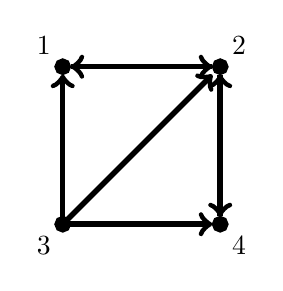
\begin{tikzpicture}[scale=2.0,line width=2pt]
\filldraw (0,0) circle (1pt); \filldraw (0,1) circle (1pt);
\filldraw (1,1) circle (1pt); \filldraw (1,0) circle (1pt);
\draw (0,1) node[anchor=south east] {1};
\draw (1,1) node[anchor=south west] {2};
\draw (1,0) node[anchor=north west] {4};
\draw (0,0) node[anchor=north east] {3};
\draw [->] (0,0) to (0,0.95);
\draw [->] (0,0) to (0.95,0);
\draw [->] (0,0) to (0.95,0.95);
\draw [->] (1,0.95) to (1,0.05);
\draw [->] (1,0.05) to (1,0.95);
\draw [->] (0.05,1) to (0.95,1);
\draw [->] (0.95,1) to (0.05,1);
\end{tikzpicture}
\end{center}
Construct the adjacency matrix $A$ and the stochastic matrix $P$
$$
A = \begin{bmatrix} 0 & 1 & 1 & 0 \\ 1 & 0 & 1 & 1 \\ 0 & 0 & 0 & 0 \\ 0 & 1 & 1 & 0 \end{bmatrix}
\hspace{10mm}
P = \begin{bmatrix} 0 & 1/2 & 1/3 & 0 \\ 1 & 0 & 1/3 & 1 \\ 0 & 0 & 0 & 0 \\ 0 & 1/2 & 1/3 & 0 \end{bmatrix}
$$
\end{example}

\begin{definition}
The {\bf Google matrix} of a directed graph $G$ is
$$
\alpha P + (1 - \alpha) \bs{v} \bs{e}^T
$$
where $P$ is the stochastic matrix of $G$, $0 < \alpha < 1$ is the {\bf teleportation parameter} \cite[p.322]{DG}, $\bs{v}$ is the {\bf teleportation distribution vector} and $\bs{e}^T = \begin{bmatrix} 1 & \cdots & 1 \end{bmatrix}$ is a vector of 1s. Note $\bs{v} \bs{e}^T$ is the matrix with vector $\bs{v}$ in every column.
\end{definition}

\begin{note}
The teleportation vector $\bs{v}$ has entries between 0 and 1 and the entries sum to 1. In other words, it is a stochastic vector. The vector $\bs{v}$ is usually chosen to be $\bs{v} = (1/N)\bs{e}$ where $N$ is the number of vertices in the graph. The stochastic matrix $\bs{v} \bs{e}^T$ then represents the process of transitioning to a random webpage with uniform probability. The Google matrix is a stochastic matrix which represents the process: at each step, do either:
\begin{itemize}
\item probability $\alpha$: click a random link on the webpage to visit another webapge
\item probability $1 - \alpha$: teleport to any webpage according to the distribution $\bs{v}$
\end{itemize}
The teleportation parameter $\alpha$ is usually chosen to be $\alpha = 0.85$.
\end{note}

\begin{proposition}
Let $G$ be a directed graph and let $P$ be the stochastic matrix for $G$. Choose parameters $0 < \alpha < 0$ and $\bs{v}$. There exists a unique steady state vector $\bs{x}$ (with entries between 0 and 1 and the entries sum to 1) such that
$$
\left( \alpha P + (1 - \alpha) \bs{v} \bs{e}^T \right) \bs{x} = \bs{x}
$$
The vector $\bs{x}$ is called the {\bf PageRank} vector and the entry $x_i$ is the PageRank of the webpage at vertex $i$. The Google search result lists the webpages in order of their PageRank.
\end{proposition}

\begin{note}
A directed graph $G$ represents a collection of webpages that contain the words in a Google search. The PageRank vector ranks the importance of the webpages for the search. There are usually hundreds of millions webpages in the graph therefore the Google matrix is HUGE! But the founders of Google showed that the power iteration algorithm converges well enough after about 50 iterations to find the webpages with the top PageRank.
\end{note}

\begin{example}
Find the Google matrix for the directed graph in the example above for $\alpha = 0.85$ and $\bs{v} = (1/N) \bs{e}$. Compute
\begin{align*}
\alpha P + (1 - \alpha) \bs{v} \bs{e}^T &=
0.85 \begin{bmatrix} 0 & 1/2 & 1/3 & 0 \\ 1 & 0 & 1/3 & 1 \\ 0 & 0 & 0 & 0 \\ 0 & 1/2 & 1/3 & 0 \end{bmatrix}
+
\frac{0.15}{4}
\begin{bmatrix} 1 & 1 & 1 & 1 \\ 1 & 1 & 1 & 1 \\ 1 & 1 & 1 & 1 \\ 1 & 1 & 1 & 1 \end{bmatrix} \\
&=
\begin{bmatrix}
0.0375 & 0.4625 & 0.3208 & 0.0375 \\
0.8875 & 0.0375 & 0.3208 & 0.8875 \\
0.0375 & 0.0375 & 0.0375 & 0.0375 \\
0.0375 & 0.4625 & 0.3208 & 0.0375
\end{bmatrix}
\end{align*}
Compute 50 iterations of the power method to approximate the PageRank vector
$$
\bs{x} \approx \begin{bmatrix} 0.2472 \\ 0.4681 \\ 0.0375 \\ 0.2472 \end{bmatrix}
$$
Clearly, vertex 2 is the most important in the graph.
\end{example}
 \newpage
\section{Exercises}

\begin{enumerate}[leftmargin=*]
\item Determine whether the statement is {\bf True} or {\bf False}.
\begin{enumerate}
\item Let $ \boldsymbol{v}_1 , \boldsymbol{v}_2 \in \mathbb{R}^2 $ be linearly independent vectors. Let $ \lambda_1 , \lambda_2 $ be real numbers. Then there exists a unique 2 by 2 matrix $ A $ with eigenvalues $ \lambda_1 , \lambda_2 $ and corresponding eigenvectors $ \boldsymbol{v}_1 , \boldsymbol{v}_2 $.
\item The singular value decomposition $A = P\Sigma Q^T$ is unique.
\item The inverse iteration algorithm (without normalization) computes a recursive sequence $ A \boldsymbol{x}_{k+1} = \boldsymbol{x}_k $ where $ \boldsymbol{x}_k $ converges to:
\begin{enumerate}
\item the largest (in absolute value $ | \lambda | $) eigenvalue of $ A $
\item an eigenvector corresponding to the largest (in absolute value $ | \lambda | $) eigenvalue of $ A $
\item the smallest (in absolute value $ | \lambda | $) eigenvalue of $ A $
\item an eigenvector corresponding to the smallest (in absolute value $ | \lambda | $) eigenvalue of $ A $
\end{enumerate}
\item In the power iteration algorithm, we divide by $ \| A \boldsymbol{x}_k \|_{\infty} $ in each step to:
\begin{enumerate}
\item make the algorithm run faster
\item prevent the entries of the vectors $ \boldsymbol{x}_k $ from becoming too large/small
\item produce a more accurate result
\end{enumerate}
\item Let $ \lambda $ be a (nonzero) eigenvalue of an invertible matrix $ A $.
\begin{enumerate}
\item $ \lambda^{-1} $ is an eigenvalue of $ A^{-1} $
\item $ \lambda $ is an eigenvalue of $ A^T $
\item $ \lambda^2 $ is an eigenvalue of $ AA^T $
\item $ \lambda $ is an eigenvalue of $ PAP^{-1} $ for any invertible matrix $ P $
\item $ \lambda \not= 0 $
\end{enumerate}
\item Let $ \boldsymbol{u} \in \mathbb{R}^n $ be a nonzero vector and let $ H = I - \frac{2}{\| \boldsymbol{u} \|^2} \boldsymbol{u} \boldsymbol{u}^T $ be the corresponding elementary reflector. Then $\lambda = -1$ is an eigenvalue of $H$ with multiplicity 1.
\item Let $ U \subset \mathbb{R}^n $ be a subspace with $ \mathrm{dim}(U) = m $ such that $ 0 < m < n$, and let $ P $ be the orthogonal projection matrix onto $ U $. Then $ \lambda = 0 $ is an eigenvalue for $ P $ with multiplicity $ m $.
\item Suppose $A$ and $B$ are symmetric $n \times n$ matrices. Then the eigenvectors of $AB$ corresponding to distinct eigenvalues are orthogonal.
\item Let $ A $ be any $ m \times n $ matrix. If $ \lambda $ is an eigenvalue of $ AA^T $ then $ \lambda $ is a real number and $ \lambda \geq 0 $.
\item Let $ A $ be any $ m \times n $ matrix. If $ \boldsymbol{v}_1 , \boldsymbol{v}_2 $ are eigenvectors of $ AA^T $ for distinct eigenvalues then $ \boldsymbol{v}_1 \cdot \boldsymbol{v}_1 = 0 $.
\item Let $ \boldsymbol{u} \in \mathbb{R}^n $ and let $ H = I - \frac{2}{\| \boldsymbol{u} \|^2} \boldsymbol{u} \boldsymbol{u}^T $ be the corresponding elementary reflector. The characteristic polynomial of $ H $ is $ (x-1)^{n-1}(x+1)$.
\item Let $ P $ be an orthogonal projection matrix. All the eigenvalues of $ P $ are either 1 or 0.
\item Let $ \lambda $ be an eigenvalue of an invertible matrix $ A $. Identify all True statements:
\begin{enumerate}
\item $ \lambda^{-1} $ is an eigenvalue of $ A^{-1} $
\item $ \lambda $ is an eigenvalue of $ A^T $
\item $ \lambda^2 $ is an eigenvalue of $ AA^T $
\item $ \lambda $ is an eigenvalue of $ PAP^{-1} $ for any invertible matrix $ P $
\item $ \lambda \not= 0 $
\end{enumerate}
\end{enumerate}
\item Let $ A $ be a $ 2 \times 2 $ matrix with eigenvalues $ \lambda_1 = 1 $ and $ \lambda_2 = 1/2 $ and corresponding eigenvectors
\[ \boldsymbol{v}_1 = \begin{bmatrix} 1 \\ 2 \end{bmatrix} \hspace{10mm} \boldsymbol{v}_2 = \begin{bmatrix} -1 \\ 1 \end{bmatrix} \]
If we choose $ \boldsymbol{x}_0 = \begin{bmatrix} 1 \\ 5 \end{bmatrix} $ then the sequence $ \boldsymbol{x}_{k+1} = A \boldsymbol{x}_k $ converges to what?
\item Find the singular value decomposition of $\displaystyle A = \left[ \begin{array}{rrr} 1 & \ \, 2 & -1 \\ 2 & 1 & 4 \end{array} \right]$.
\item Suppose $ A $ is a symmetric $ 3 \times 3 $ matrix with distinct eigenvalues $ \lambda_1 , \lambda_2 , \lambda_3 $ and eigenvectors
\[ \boldsymbol{v}_1 = \begin{bmatrix} 1 \\ 1 \\ 1 \end{bmatrix} \hspace{10mm} \boldsymbol{v}_2 = \begin{bmatrix} 1 \\ 0 \\ -1 \end{bmatrix} \]
Determine eigenvector $ \boldsymbol{v}_3 $ for eigenvalue $ \lambda_3 $.
\item Find the singular value decomposition of $ \displaystyle A = \left[ \begin{array}{rrr} 1 & 1 & 1 \\ -1 & 2 & -1 \\ 1 & 0 & -1 \end{array} \right] $.
\item Determine whether the statement is {\bf True} or {\bf False}. (Assume all data matrices are normalized.)
\begin{enumerate}
\item Let $X$ be a $n \times p$ data matrix and let $\bs{x}_i , \bs{x}_j \in \mathbb{R}^p$ be two different rows of $X$ such that $\| \bs{x}_i \| < \| \bs{x}_j \|$. If $\bs{w}_1$ is the first weight vector of $X$, then $| \bs{x}_i \cdot \bs{w}_1 | < | \bs{x}_j \cdot \bs{w}_1 |$.
\item Let $X$ be a $n \times p$ data matrix and let $\bs{x}_i , \bs{x}_j \in \mathbb{R}^p$ be two different rows of $X$ such that $\bs{x}_i \cdot \bs{x}_j = 0$. If $\bs{w}_1$ is the first weight vector of $X$ and $\bs{x}_i \cdot \bs{w}_1 = 0$ then $\bs{x}_j \cdot \bs{w}_1 = 0$.
\item Let $X$ be a $n \times 2$ data matrix and let $Y$ be the matrix with the same columns as $X$ but switched. (In other words, the first column of $Y$ is the same as the second column of $X$, and the second column of $Y$ is the first column of $X$.) If $X$ and $Y$ represent the same set of data points, then all the singular values of $X$ equal.
\item Let $X$ be a $n \times 2$ data matrix and let $Y$ be the matrix with the same columns as $X$ but switched. (In other words, the first column of $Y$ is the same as the second column of $X$, and the second column of $Y$ is the first column of $X$.) If $X$ and $Y$ represent the same set of data points, then $\bs{w}_1 = \begin{bmatrix} 1/\sqrt{2} & 1/\sqrt{2} \end{bmatrix}^T$.
\item It is necessary to compute all the eigenvectors of the Google matrix to find the PageRank vector of a directed graph.
\end{enumerate}
\item Find the weight vectors for the data matrix $X$ representing the points:
\begin{center}
\includegraphics[width=3in]{03_04_ex01.png}
\end{center}
\item Suppose $X$ is a $100 \times 4$ data matrix such that
$$
X^T X = \begin{bmatrix} 2 & 0 & 0 & 0 \\ 0 & 1.5 & 0 & 0 \\ 0 & 0 & 2 & 1 \\ 0 & 0 & 1 & 2 \end{bmatrix}
$$
Find all the weight vectors of $X$.
\item Suppose we want to solve a system $A \bs{x} = \bs{b}$. A small change $\Delta \bs{b}$ produces a change in the solution
$$
A(\bs{x} + \Delta \bs{x}) = \bs{b} + \Delta \bs{b}
$$
Describe the unit vector $\Delta \bs{b}$ that will produce the largest change $\| \Delta \bs{x} \|$.
\item Find the rank 2 pseudo inverse
$$
A_2^+ = \frac{1}{\sigma_1} \bs{q}_1 \bs{p}_1^T + \frac{1}{\sigma_2} \bs{q}_2 \bs{p}_2^T
$$
of the matrix
$$
A = \left[ \begin{array}{rrr} 1 & 1 & 1 \\ 1 & 0 & -2 \\ 1 & -1 & 1 \end{array} \right]
$$
(Note: the columns of $A$ are orthogonal.)
\item Let $A$ be a $m \times n$ matrix with singular value decomposition $A = P \Sigma Q^T$. Let $k < \min\{m,n\}$ and let
$$
A_k = \sum_{i=1}^k \sigma_i \bs{p}_i \bs{q}_i^T
$$
Describe the singular value decomposition of $A - A_k$.
%\item Consider a Toeplitz matrix of the form
%$$
%A = 
%\begin{bmatrix}
%a & b & & & \\
%c & a & b & & \\
% &  & \ddots & & \\
% & & c & a & b \\
% & & & c & a
%\end{bmatrix}
%$$
%and an image matrix $X$
%\begin{enumerate}
%\item If $c > a > b > 0$, would the blurred image $AX$ look more blurred upward or downward?
%\item If $c > a > b > 0$, would the blurred image $XA^T$ look more blurred to the right or left?
%\end{enumerate}
\item Consider the same directed graph as in the example in the section on PageRank:
\begin{center}
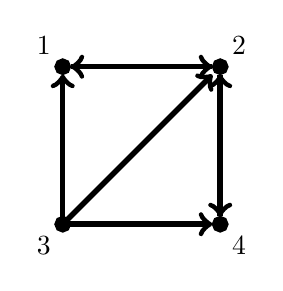
\begin{tikzpicture}[scale=2.0,line width=2pt]
\filldraw (0,0) circle (1pt); \filldraw (0,1) circle (1pt);
\filldraw (1,1) circle (1pt); \filldraw (1,0) circle (1pt);
\draw (0,1) node[anchor=south east] {1};
\draw (1,1) node[anchor=south west] {2};
\draw (1,0) node[anchor=north west] {4};
\draw (0,0) node[anchor=north east] {3};
\draw [->] (0,0) to (0,0.95);
\draw [->] (0,0) to (0.95,0);
\draw [->] (0,0) to (0.95,0.95);
\draw [->] (1,0.95) to (1,0.05);
\draw [->] (1,0.05) to (1,0.95);
\draw [->] (0.05,1) to (0.95,1);
\draw [->] (0.95,1) to (0.05,1);
\end{tikzpicture}
\end{center}
As $\alpha \to 1$, describe what happens to the PageRank $x_3$ of vertex 3.
\item Let $G$ be the complete directed graph with $N$ vertices. In other words, there is an edge from each vertex to every other vertex in $G$ (excluding edges from a vertex to itself). Describe the Google matrix and the PageRank vector for the complete directed graph.
\item Find the Google matrix $\alpha P + (1 - \alpha) \bs{v} \bs{e}^T$ for the directed graph
\begin{center}
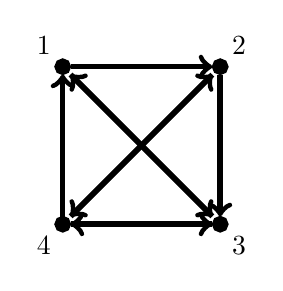
\begin{tikzpicture}[scale=2.0,line width=2pt]
\filldraw (0,0) circle (1pt); \filldraw (0,1) circle (1pt);
\filldraw (1,1) circle (1pt); \filldraw (1,0) circle (1pt);
\draw (0,1) node[anchor=south east] {1};
\draw (1,1) node[anchor=south west] {2};
\draw (1,0) node[anchor=north west] {3};
\draw (0,0) node[anchor=north east] {4};
\draw [->] (0,0) to (0,0.95);
\draw [->] (0.05,0) to (0.95,0);
\draw [->] (0.95,0) to (0.05,0);
\draw [->] (0.05,0.05) to (0.95,0.95);
\draw [->] (0.95,0.95) to (0.05,0.05);
\draw [->] (0.05,0.95) to (0.95,0.05);
\draw [->] (0.95,0.05) to (0.05,0.95);
\draw [->] (1,0.95) to (1,0.05);
\draw [->] (0.05,1) to (0.95,1);

%\draw [->] (0.05,1.05) to[out=45,in=135] (0.95,1.07);
%\draw [->] (0.05,1) to[out=0,in=90] (1,0.1);
%\draw [->] (0.95,0) to[out=180,in=-90] (0,0.9);
%\draw [->] (0.05,0.05) to[out=45,in=135] (0.9,0.05);
%\draw [->] (0.95,-0.05) to[in=-45,out=225] (0.07,-0.07);
%\draw [->] (-0.05,0.05) to[out=135,in=225] (-0.1,0.95);
%\draw [->] (1.05,0.95) to[out=-45,in=45] (1.1,0.05);
%\draw [->] (0,0.05) to[out=90,in=180] (0.9,1);
%\draw [->] (1,0.95) to[out=-90,in=0] (0.1,0);
\end{tikzpicture}
\end{center}
using teleportation parameter $\alpha=0.5$ and uniform distribution vector $\bs{v}$. Let $\bs{x}_0 = \begin{bmatrix} 1 & 0 & 0 & 0 \end{bmatrix}^T$ and use Python to compute 50 iterations of the power method to approximate the PageRank vector.
\item Find the Google matrix $\alpha P + (1 - \alpha) \bs{v} \bs{e}^T$ for the directed graph in the previous exercise using teleportation parameter $\alpha=0.8$ and distribution vector $\bs{v} =  \begin{bmatrix} 0 & 1/2 & 1/2 & 0 \end{bmatrix}^T$. Let $\bs{x}_0 = \begin{bmatrix} 1 & 0 & 0 & 0 \end{bmatrix}^T$ and use Python to compute 50 iterations of the power method to approximate the PageRank vector.
\end{enumerate}

%%%%%%%%%%%%%%%%%%%%%%%%%%%%%%%%%%%%%%%%%%%%%%%%%%

\chapter{Discrete Fourier Transform} \newpage
\section{Review: Complex Numbers, Vectors and Matrices}

\begin{bigidea}
A complex number can be represented in the form $z = a + i b$ and also in polar form $z = r e^{i \theta}$. The set of vectors of length $n$ with complex entries is a complex vector space $\mathbb{C}^n$ with inner product $\langle \bs{u} , \bs{v} \rangle = \bs{u}^T \overline{\bs{v}}$.
\end{bigidea}

\begin{definition}
A {\bf complex number} \cite[p.597]{KN} is of the form
$$
z = a + i b
$$
where $i = \sqrt{-1}$ and $a,b \in \mathbb{R}$. The complex number $i$ satisfies $i^2 = -1$, the real number $a$ is called the {\bf real part} of $z$ and $b$ is the {\bf imaginary part}, and we write $\mathrm{Re}(z) = a$ and $\mathrm{Im}(z) = b$. The {\bf polar form} \cite[p.601]{KN} of a complex number $z = a + i b$ is
$$
z = r e^{i \theta}
$$
where $r = \sqrt{a^2 + b^2}$ and $\theta = \arctan(b/a)$. We visualize the {\bf set of complex numbers} $\mathbb{C}$ as a 2-dimensional real vector space:
\begin{center}
\begin{tikzpicture}[scale=2]
\draw [->] (-1,0) -- (1,0) node[right] {Re};
\draw [->] (0,-0.5) -- (0,1) node[above] {Im};
\filldraw (0.8,0.8) circle (1pt) node[right] {$z = a + ib$};
\draw[dashed] (0,0.8) -- (0.8,0.8) -- (0.8,0);
\draw[dashed] (0,0) -- (0.8,0.8) node[pos=0.5,above] {$r$};
\draw (0.4,0) node[below right] {$a$};
\draw (0.8,0.4) node[right] {$b$};
\draw (0.3,0.14) node {$\theta$};
\end{tikzpicture}
\end{center}
\end{definition}

\begin{theorem}
{\bf Euler's formula} is
$$
e^{i \theta} = \cos \theta + i \sin \theta
$$
See \cite[p.602]{KN}.
\end{theorem}

\begin{definition}
Let $z = a + ib$ and $z = re^{i \theta}$ in polar form.
\begin{enumerate}
\item The {\bf modulus} of $z$ is $|z| = r = \sqrt{a^2 + b^2}$.
\item The {\bf angle} (or {\bf argument}) of $z$ is $\angle z = \theta = \arctan(b/a)$ (or $\mathrm{arg}(z) = \theta$).
\item The {\bf conjugate} of $z$ is $\overline{z} = a - ib = re^{- i \theta}$.
\end{enumerate}
See \cite[p.599]{KN}.
\end{definition}

\begin{proposition}
$$
z^{-1} = \frac{\overline{z} \ \, }{|z|^2}
$$

\begin{proof}
Let $z = a + ib$. Then
$$
z^{-1} = \frac{1}{z} = \frac{\overline{z}}{z \overline{z}}
$$
and we see
$$
z \overline{z} = (a + ib)(a - ib) = a^2 + b^2 = |z|^2
$$
\end{proof}
\end{proposition}

\begin{definition}
The {\bf complex vector space} $\mathbb{C}^n$ \cite[p.461]{KN} is the set of vectors of length $n$
$$
\bs{v} = \begin{bmatrix} v_1 \\ \vdots \\ v_n \end{bmatrix}
$$
with complex entries $v_1, \dots, v_n \in \mathbb{C}$. The {\bf conjugate} of a vector $\bs{v} \in \mathbb{C}^n$ is given by the conjugate of each entry
$$
\overline{\bs{v}} = \begin{bmatrix} \overline{v}_1 \\ \vdots \\ \overline{v}_n \end{bmatrix}
$$
\end{definition}

\begin{definition}
The {\bf standard inner product} \cite[p.462]{KN} of vectors $\bs{u},\bs{v} \in \mathbb{C}^n$ is
$$
\langle \bs{u} , \bs{v} \rangle = \bs{u}^T \overline{ \bs{v} } = u_1 \overline{v}_1 + \cdots + u_n \overline{v}_n
$$
\end{definition}

\begin{proposition}
Let $\bs{u} , \bs{v} \in \mathbb{C}^n$ and let $c \in \mathbb{C}$.
\begin{enumerate}
\item $\langle c \, \bs{u} , \bs{v} \rangle = c \, \langle \bs{u} , \bs{v} \rangle$
\item $\langle \bs{u} , c \, \bs{v} \rangle = \overline{c} \, \langle \bs{u} , \bs{v} \rangle$
\item $\langle \bs{u} , \bs{v} \rangle = \overline{\langle \bs{v} , \bs{u} \rangle}$
\item $\langle \bs{v} , \bs{v} \rangle \geq 0$ for all $\bs{v}$, and $\langle \bs{v} , \bs{v} \rangle = 0$ if and only if $\bs{v} = \bs{0}$ is the zero vector.
\end{enumerate}
See \cite[p.462]{KN}.
\end{proposition}

\begin{definition}
The {\bf norm} \cite[p.463]{KN} of $\bs{v} \in \mathbb{C}^n$ is
$$
\| \bs{v} \| = \sqrt{ \langle \bs{v} , \bs{v} \rangle } = \sqrt{ |v_1|^2 + \cdots + |v_n|^2 }
$$
\end{definition}

\begin{definition}
Complex vectors $\bs{u} , \bs{v} \in \mathbb{C}^n$ are {\bf orthogonal} \cite[p.466]{KN} if $ \langle \bs{u} , \bs{v} \rangle = 0$.
\end{definition}

\begin{definition}
A complex matrix $A$ is {\bf hermitian} \cite[p.464]{KN} if $A = \overline{A}^T$.
\end{definition}

\begin{proposition}
If $A$ is hermitian then $\langle A \bs{u} , \bs{v} \rangle = \langle \bs{u} , A \bs{v} \rangle$ for all $\bs{u} , \bs{v} \in \mathbb{C}^n$.

\begin{proof}
See \cite[p.464]{KN}.
\end{proof}
\end{proposition}

\begin{definition}
A complex matrix $A$ is {\bf unitary} \cite[p.466]{KN} if $A^{-1} = \overline{A}^T$.
\end{definition}

\begin{proposition}
If $A$ is unitary then $\langle A \bs{u} , A \bs{v} \rangle = \langle \bs{u} , \bs{v} \rangle$ for all $\bs{u} , \bs{v} \in \mathbb{C}^n$.

\begin{proof}
See \cite[p.466]{KN}.
\end{proof}
\end{proposition}


\section{Discrete Fourier Transform}

\begin{bigidea}
The discrete Fourier transform (DFT) is the orthogonal projection onto the Fourier basis vectors $\bs{f}_0 , \dots, \bs{f}_{N-1}$.
\end{bigidea}

\begin{definition}
An {\bf $N$th root of unity} is a complex number $\omega$ such that $\omega^N = 1$.
\end{definition}

\begin{proposition}
Let $\omega_N = e^{2 \pi i / N}$. Then $\omega_N$ is an $N$th root of unity and $1,\omega_N,\omega_N^2,\dots,\omega_N^{N-1}$ are all the $N$th roots of unity.
\end{proposition}

\begin{proposition}
Let $\omega_N = e^{2 \pi i / N}$.
\begin{enumerate}
\item $\overline{\omega}_N = \omega_N^{-1} = \omega_N^{N-1}$
\item $\displaystyle \omega_N^k = \cos\left( \frac{2 \pi k}{N} \right) + i \sin \left( \frac{2 \pi k}{N} \right)$
\end{enumerate}
\end{proposition}

\begin{proposition}
Let $\omega_N = e^{2 \pi i / N}$ and let $k$ be an integer such that $0<k<N$. Then
$$
\sum_{n=0}^{N-1} \omega_N^{nk} = 0
$$

\begin{proof}
The sum is a geometric series
$$
\sum_{n=0}^{N-1} r^n = \frac{1 - r^N}{1 - r}
$$
and so with $r = \omega_N^k$ we have
$$
\sum_{n=0}^{N-1} \omega_N^{nk} =  \frac{1 - \omega_N^{kN}}{1 - \omega_N^k} = 0
$$
since $\omega_N^{kN} = 1$ and $\omega_N^k \not= 1$.
\end{proof}
\end{proposition}

\begin{definition}
The {\bf standard basis} of $\mathbb{C}^N$ is $\bs{e}_0 , \dots, \bs{e}_{N-1}$ where $\bs{e}_k$ is the vector with all 0s except 1 in index $k$
$$
\bs{e}_k = \begin{bmatrix} \bs{0} \\ 1 \\ \bs{0} \end{bmatrix} \leftarrow \text{index } k
$$
Use 0-indexing (as in Python) such that the first entry is at index 0. For example, for $N=3$,
$$
\bs{e}_0 = \begin{bmatrix} 1 \\ 0 \\ 0 \end{bmatrix} \hspace{10mm}
\bs{e}_1 = \begin{bmatrix} 0 \\ 1 \\ 0 \end{bmatrix} \hspace{10mm}
\bs{e}_2 = \begin{bmatrix} 0 \\ 0 \\ 1 \end{bmatrix}
$$
\end{definition}

\begin{definition}
Let $N$ be a positive integer and let $\omega_N = e^{2 \pi i / N}$. The {\bf Fourier basis} of $\mathbb{C}^N$ is $\bs{f}_0 , \dots, \bs{f}_{N-1}$ where
$$
\renewcommand{\arraystretch}{1.5}
\bs{f}_k = \begin{bmatrix} 1 \\ \omega^k_N \\ \omega^{2k}_N \\ \vdots \\ \omega^{(N-1)k}_N \end{bmatrix}
\renewcommand{\arraystretch}{1}
$$
\end{definition}

\begin{example}
For $N=2$, $\omega_2 = -1$ and the Fourier basis of $\mathbb{C}^2$ is
$$
\bs{f}_0 = \left[ \begin{array}{r} 1 \\ 1 \end{array} \right]
\hspace{10mm}
\bs{f}_1 = \left[ \begin{array}{r} 1 \\ -1 \end{array} \right]
$$
For $N=3$, $\omega_3 = e^{2 \pi i/3} = (-1 + \sqrt{3}i)/2$ and the Fourier basis of $\mathbb{C}^3$ is
$$
\bs{f}_0 = \left[ \begin{array}{r} 1 \\ 1 \\ 1 \end{array} \right]
\hspace{10mm}
\bs{f}_1 = \left[ \begin{array}{c} 1 \\ (-1 + \sqrt{3}i)/2 \\ (-1 - \sqrt{3}i)/2 \end{array} \right]
\hspace{10mm}
\bs{f}_2 = \left[ \begin{array}{c} 1 \\ (-1 - \sqrt{3}i)/2 \\ (-1 + \sqrt{3}i)/2 \end{array} \right]
$$
For $N=4$, $\omega_4 = i$ and the Fourier basis of $\mathbb{C}^4$ is
$$
\bs{f}_0 = \left[ \begin{array}{r} 1 \\ 1 \\ 1 \\ 1 \end{array} \right]
\hspace{10mm}
\bs{f}_1 = \left[ \begin{array}{r} 1 \\ i \\ -1 \\ -i \end{array} \right]
\hspace{10mm}
\bs{f}_2 = \left[ \begin{array}{r} 1 \\ -1 \\ 1 \\ -1 \end{array} \right]
\hspace{10mm}
\bs{f}_3 = \left[ \begin{array}{r} 1 \\ -i \\ -1 \\ i \end{array} \right]
$$
\end{example}

\begin{proposition}
The Fourier basis $\bs{f}_0 , \dots, \bs{f}_{N-1}$ satisfies
$$
\langle \bs{f}_k , \bs{f}_{\ell} \rangle = \left\{ \begin{array}{cl} N & \text{if } k = \ell \\ 0 & \text{otherwise} \end{array} \right.
$$
Therefore the Fourier basis is an orthogonal basis of $\mathbb{C}^N$.

\begin{proof}
Compute
$$
\langle \bs{f}_k , \bs{f}_{\ell} \rangle
= \sum_{n=0}^{N-1} \omega_N^{nk} \omega_N^{-n\ell}
= \sum_{n=0}^{N-1} \omega_N^{n(k -\ell)}
$$
We showed in a previous proposition that the sum is equal to 0 if $k \not= \ell$. If $k = \ell$ then clearly the sum is equal to $N$.
\end{proof}
\end{proposition}

\begin{proposition}
Let $0<k<N$. Then
$$
\overline{\bs{f}}_k = \bs{f}_{N-k}
$$
\begin{proof}
By definition and using $\omega_N^N = 1$ we have
$$
\renewcommand{\arraystretch}{1.5}
\overline{\bs{f}}_k = \begin{bmatrix} 1 \\ \overline{\omega}^k_N \\ \overline{\omega}^{2k}_N \\ \vdots \\ \overline{\omega}^{(N-1)k}_N \end{bmatrix}
= \begin{bmatrix} 1 \\ \omega^{-k}_N \\ \omega^{-2k}_N \\ \vdots \\ \omega^{-(N-1)k}_N \end{bmatrix}
= \begin{bmatrix} 1 \\ \omega^{N-k}_N \\ \omega^{2(N-k)}_N \\ \vdots \\ \omega^{(N-1)(N-k)}_N \end{bmatrix}
= \bs{f}_{N-k}
\renewcommand{\arraystretch}{1}
$$
\end{proof}
\end{proposition}

\begin{definition}
Let $\bs{x} \in \mathbb{C}^N$. The {\bf discrete Fourier transform} of $\bs{x}$ is
$$
\mathrm{DFT}(\bs{x}) = F_N \bs{x}
$$
where $F_N$ is the {\bf Fourier matrix}
$$
\renewcommand{\arraystretch}{1.5}
F_N =
\begin{bmatrix} & & \overline{\bs{f}}^T_0 & & \\ & & \overline{\bs{f}}^T_1 & & \\ & & \vdots & & \\ & & \overline{\bs{f}}^T_{N-1} & & \end{bmatrix}
=
\renewcommand{\arraystretch}{1.25}
\begin{bmatrix}
1 & 1 & 1 & \cdots & 1 \\
1 & \overline{\omega}_N & \overline{\omega}_N^2 & \cdots & \overline{\omega}_N^{N-1} \\
1 & \overline{\omega}_N^2 & \overline{\omega}_N^4 & \cdots & \overline{\omega}_N^{2(N-1)} \\
1 & \vdots & \vdots & \ddots & \vdots \\
1 & \overline{\omega}_N^{N-1} & \overline{\omega}_N^{2(N-1)} & \cdots & \overline{\omega}_N^{(N-1)^2}
\end{bmatrix}
\renewcommand{\arraystretch}{1}
$$
\end{definition}

\begin{note}
Expand $\bs{x}$ in terms of the Fourier basis
$$
\bs{x} = \frac{\langle \bs{x} , \bs{f}_0 \rangle}{\langle \bs{f}_0 , \bs{f}_0 \rangle} \bs{f}_0 + \cdots + \frac{\langle \bs{x} , \bs{f}_{N-1} \rangle}{\langle \bs{f}_{N-1} , \bs{f}_{N-1} \rangle} \bs{f}_{N-1}
$$
Note that $\langle \bs{f}_k , \bs{f}_k \rangle = N$ for each $k=0,\dots,N-1$ and write as matrix multiplication
$$
\bs{x} = \frac{1}{N}
\begin{bmatrix} & & \\ \bs{f}_0 & \cdots & \bs{f}_{N-1} \\ & & \end{bmatrix}
\begin{bmatrix} \langle \bs{x} , \bs{f}_0 \rangle \\ \langle \bs{x} , \bs{f}_1 \rangle \\ \vdots \\ \langle \bs{x} , \bs{f}_{N-1} \rangle \end{bmatrix}
= \frac{1}{N} 
\begin{bmatrix} & & \\ \bs{f}_0 & \cdots & \bs{f}_{N-1} \\ & & \end{bmatrix}
\renewcommand{\arraystretch}{1.5}
\begin{bmatrix} & & \overline{\bs{f}}^T_0 & & \\ & & \overline{\bs{f}}^T_1 & & \\ & & \vdots & & \\ & & \overline{\bs{f}}^T_{N-1} & & \end{bmatrix}
\renewcommand{\arraystretch}{1}
\bs{x}
$$
Therefore $F_N \bs{x}$ is the vector of coefficients of $\bs{x}$ with respect to the Fourier basis (up to multiplication by $N$).
\end{note}

\begin{definition}
The DFT is used to study sound, images and any kind of information that can be represented by a vector $\bs{x} \in \mathbb{C}^N$. Therefore, in the context of the DFT, we use the term {\bf signal} to refer to a (column) vector $\bs{x} \in \mathbb{C}^N$ and we use the notation
$$
\bs{x} = \begin{bmatrix} \ x_0 & x_1 & x_2 & \cdots & x_{N-1} \ \end{bmatrix}^T
\hspace{10mm}
\bs{x}[n] = x_n
$$
\end{definition}

\begin{proposition}
Let $\bs{x}$ be a real signal (that is, $\bs{x}[k] \in \mathbb{R}$ for each $k=0,\dots,N-1$) and let $\bs{y} = \mathrm{DFT}(\bs{x})$. Then
$$
\overline{\bs{y}[k]} = \bs{y}[N-k]
$$

\begin{proof}
Compute from the definition
\begin{align*}
\overline{\bs{y}[k]} &= \overline{\langle \bs{x} , \bs{f}_k \rangle} =  \langle \bs{f}_k , \bs{x} \rangle = \sum_{n=0}^{N-1} \omega_N^{nk} \overline{x}_n \\
&= \sum_{n=0}^{N-1} \omega_N^{nk-nN} x_n \\
&= \sum_{n=0}^{N-1} \omega_N^{-(N-k)n} x_n = \bs{y}[N-k]
\end{align*}

\end{proof}
\end{proposition}

\begin{proposition}
For each $k=0,\dots,N-1$, we have
$$
\mathrm{DFT}(\bs{f}_k) = N \bs{e}_k
$$
where $\bs{e}_k$ is the $k$th standard basis vector.

\begin{proof}
By definition of DFT and the fact $\langle \bs{f}_k , \bs{f}_{\ell} \rangle = 0$ when $k \not= \ell$ and $\langle \bs{f}_k , \bs{f}_k \rangle = N$, compute
$$
\mathrm{DFT}(\bs{f}_k) = 
\renewcommand{\arraystretch}{1.5}
\begin{bmatrix} & & \overline{\bs{f}}^T_0 & & \\ & & \vdots & & \\ & & \overline{\bs{f}}^T_{N-1} & & \end{bmatrix} \bs{f}_k
=
\begin{bmatrix} \langle \bs{f}_k , \bs{f}_0 \rangle \\ \vdots \\ \langle \bs{f}_k , \bs{f}_{N-1} \rangle \end{bmatrix}
=
\begin{bmatrix} \bs{0} \\ N \\ \bs{0} \end{bmatrix} \leftarrow \text{index } k
\renewcommand{\arraystretch}{1}
$$
and so $\mathrm{DFT}(\bs{f}_k) = N \bs{e}_k$.
\end{proof}
\end{proposition}

\begin{definition}
Let $\bs{y} \in \mathbb{C}^N$. The {\bf inverse discrete Fourier transform} of $\bs{y}$ is
$$
\mathrm{IDFT}(\bs{y}) = \frac{1}{N} \overline{F}^T_N \bs{y}
$$
\end{definition}

\begin{note}
The Fourier matrix $F_N$ is {\it not} unitary however the matrix $\frac{1}{\sqrt{N}} F_N$ is unitary.
\end{note}

\section{Frequency, Amplitude and Phase}

\begin{bigidea}
The DFT of a signal computes the amplitude and phase of each frequency in the signal.
\end{bigidea}

\begin{definition}
The DFT is used to study sound, images and any kind of information that can be represented by a vector $\bs{x} \in \mathbf{C}^N$. Therefore, in the context of the DFT, we use the term {\bf signal} to refer to a vector $\bs{x} \in \mathbf{C}^N$ and we use the notation $\bs{x}[n] = x_n$ to refer to the entries
$$
\bs{x} = \begin{bmatrix} \ x_0 & x_1 & x_2 & \cdots & x_{N-1} \ \end{bmatrix}^T
$$
\end{definition}

\begin{definition}
Let $N$ be a positive integer and let
$$
\bs{n} = \begin{bmatrix} 0 & 1 & 2 & \cdots & N-1 \end{bmatrix}^T
\hspace{10mm}
\bs{t} = (1/N) \bs{n} = \begin{bmatrix} 0 & 1/N & 2/N & \cdots & (N-1)/N \end{bmatrix}^T
$$ 
A {\bf sinusoid} is a signal of the form
$$
\bs{x} = A \cos(2\pi k \bs{t} + \phi)
$$
where $k$ is the {\bf frequency} (in periods per $N$ samples), $A$ is the {\bf amplitude} and $\phi$ is the {\bf phase}. Here we use vector notation
$$
A \cos(2\pi k \bs{t} + \phi) = \begin{bmatrix} A \cos(\phi) \\ A \cos(2\pi k (1/N) + \phi) \\ A \cos(2\pi k (2/N) + \phi) \\ \vdots \\ A \cos(2\pi k (N-1)/N + \phi) \end{bmatrix}
$$
\end{definition}

\begin{example}
Let $N = 8$ and so
\begin{align*}
\bs{n} &= \begin{bmatrix} 0 & 1 & 2 & 3 & 4 & 5 & 6 & 7 \end{bmatrix}^T \\
\bs{t} &= \begin{bmatrix} 0 & 1/8 & 1/4 & 3/8 & 1/2 & 5/8 & 3/4 & 7/8 \end{bmatrix}^T
\end{align*}
Consider the signal
$$
\bs{x} = \cos(2 \pi \bs{t} ) = \begin{bmatrix} 1 & 1/\sqrt{2} & 0 & -1/\sqrt{2} & -1 & -1/\sqrt{2} & 0 & 1/\sqrt{2} \end{bmatrix}^T
$$
and sketch the signal as a stemplot
\begin{center}
\begin{tikzpicture}
\draw [->] (0,0) -- (8,0) node[below right] {$n$}; \draw [->] (0,-1.5) -- (0,1.5) node[above left] {$\bs{x}[n]$};
\draw (0.1,1) -- (-0.1,1) node[left] {1}; \draw (0.1,-1) -- (-0.1,-1) node[left] {$-1$};
\foreach \x/\y in { 0/1 , 1/0.7071 , 2/0 , 3/-0.7071 , 4/-1 , 5/-0.7071 , 6/0 , 7/0.7071} { \filldraw (\x,0) -- (\x,\y) circle[radius=2pt]; }
\foreach \k in {0,...,7} { \draw (\k,0) node[below right] {$\k$}; }
\end{tikzpicture}
\end{center}

Now consider the signal
$$
\bs{x} = \cos(4 \pi \bs{t} ) = \begin{bmatrix} 1 & 0 & -1 & 0 & 1 & 0 & -1 \end{bmatrix}^T
$$
and sketch the signal as a stemplot
\begin{center}
\begin{tikzpicture}
\draw [->] (0,0) -- (8,0) node[below right] {$n$}; \draw [->] (0,-1.5) -- (0,1.5) node[above left] {$\bs{x}[n]$};
\draw (0.1,1) -- (-0.1,1) node[left] {1}; \draw (0.1,-1) -- (-0.1,-1) node[left] {$-1$};
\foreach \x/\y in { 0/1 , 1/0 , 2/-1 , 3/0 , 4/1 , 5/0 , 6/-1 , 7/0} { \filldraw (\x,0) -- (\x,\y) circle[radius=2pt]; }
\foreach \k in {0,...,7} { \draw (\k,0) node[below right] {$\k$}; }
\end{tikzpicture}
\end{center}

\end{example}

\begin{proposition}
\begin{align*}
\bs{f}_k & = \cos(2 \pi k \bs{t}) + i \sin(2 \pi k \bs{t}) \\
\frac{1}{2} \left( \bs{f}_k + \overline{\bs{f}}_k \right) &= \cos(2 \pi k \bs{t}) \\
\frac{1}{2i} \left( \bs{f}_k - \overline{\bs{f}}_k \right) &= \sin(2 \pi k \bs{t})
\end{align*}

\begin{proof}
We showed in a previous proposition that
$$
\omega_N^k = \cos\left( \frac{2 \pi k}{N} \right) + i \sin \left( \frac{2 \pi k}{N} \right)
$$
therefore
$$
\bs{f}_k =
\renewcommand{\arraystretch}{1.5}
\begin{bmatrix} 1 \\ \omega^k_N \\ \omega^{2k}_N \\ \vdots \\ \omega^{(N-1)k}_N \end{bmatrix}
=
\begin{bmatrix} 1 \\ \cos(2\pi k (1/N)) + i \sin(2\pi k (1/N)) \\ \cos(2\pi k (2/N)) + i \sin(2\pi k (2/N)) \\ \vdots \\ \cos(2\pi k (N-1)/N) + i \sin(2\pi k (N-1)/N) \end{bmatrix}
= \cos(2 \pi k \bs{t}) + i \sin(2 \pi k \bs{t})
$$
Further,
\begin{align*}
\omega_N^{nk} + \omega_N^{-nk} &= \cos\left( \frac{2 \pi n k}{N} \right) + i \sin \left( \frac{2 \pi n k}{N} \right) + \cos\left( \frac{2 \pi n k}{N} \right) - i \sin \left( \frac{2 \pi n k}{N} \right) \\
&= 2\cos\left( \frac{2 \pi n k}{N} \right) 
\end{align*}
Therefore
$$
\bs{f}_k + \overline{\bs{f}}_k =
\begin{bmatrix} 1 \\ \omega^k_N \\ \omega^{2k}_N \\ \vdots \\ \omega^{(N-1)k}_N \end{bmatrix} +
\begin{bmatrix} 1 \\ \omega^{-k}_N \\ \omega^{-2k}_N \\ \vdots \\ \omega^{-(N-1)k}_N \end{bmatrix}
= \begin{bmatrix} 2 \\ 2\cos( 2 \pi k/N ) \\ 2\cos( 2 \pi n (2k)/N ) \\ \vdots \\ 2\cos( 2 \pi (N-1) k/N ) \end{bmatrix}
= 2 \cos(2 \pi k \bs{t})
\renewcommand{\arraystretch}{1}
$$
The last equality is proved similarly.
\end{proof}
\end{proposition}

\begin{proposition}
Let $\bs{x} = A \cos(2 \pi k \bs{t} + \phi)$. Then
$$
\mathrm{DFT}(\bs{x}) = \frac{AN}{2} e^{i \phi} \, \bs{e}_k + \frac{AN}{2} e^{-i \phi} \, \bs{e}_{N-k}
$$

\begin{proof}
We proved in a previous proposition
$$
\cos(2 \pi k \bs{t} ) = \frac{1}{2} \left( \bs{f}_k + \overline{\bs{f}}_k \right) = \frac{1}{2} \left( \bs{f}_k + \bs{f}_{N-k} \right)
$$
and we also showed that
$$
\mathrm{DFT}( \bs{f}_k ) = N \bs{e}_k
$$
Compute
$$
\mathrm{DFT}(\cos(2 \pi k \bs{t} )) = \frac{1}{2} \mathrm{DFT}(\left( \bs{f}_k + \bs{f}_{N-k} \right)) = \frac{1}{2} \left( N\bs{e}_k + N \bs{e}_{N-k} \right)
$$
Similarly, compute
$$
\mathrm{DFT}(\sin(2 \pi k \bs{t} )) = \frac{1}{2i} \mathrm{DFT}(\left( \bs{f}_k - \bs{f}_{N-k} \right)) = \frac{1}{2i} \left( N\bs{e}_k - N \bs{e}_{N-k} \right)
$$
Use the trigonometric identity
$$
\cos(\alpha + \beta) = \cos \alpha \cos \beta - \sin \alpha \sin \beta
$$
to find
\begin{align*}
\mathrm{DFT}(\bs{x}) &= \mathrm{DFT}(A \cos(2 \pi k \bs{t} + \phi)) \\
&= A \cos(\phi) \, \mathrm{DFT}(\cos(2 \pi k \bs{t}))  - A  \sin(\phi) \, \mathrm{DFT}(\sin(2 \pi k \bs{t})) \\
&= \frac{A \cos(\phi)}{2} \left( N\bs{e}_k + N \bs{e}_{N-k} \right) - \frac{A \sin(\phi)}{2i} \left( N\bs{e}_k - N \bs{e}_{N-k} \right) \\
&= \frac{AN ( \cos(\phi) + i \sin(\phi) )}{2} \, \bs{e}_k + \frac{AN (\cos(\phi) - i\sin(\phi))}{2} \, \bs{e}_{N-k} \\
&= \frac{AN}{2} e^{i \phi} \, \bs{e}_k + \frac{AN}{2} e^{-i \phi} \, \bs{e}_{N-k}
\end{align*}
\end{proof}
\end{proposition}

\begin{definition}
The {\bf magnitude stemplot} of a complex vector $\bs{y} \in \mathbb{C}^N$ is the plot of the magnitude $| \bs{y}[n] |$ versus the index $n$. The {\bf angle stemplot} of $\bs{y}$ is the plot of the argument $\angle \bs{y}[n]$ versus the index $n$.
\end{definition}

\begin{example}
Let $N=8$ and compute the DFT of the sinusoid $\bs{x} = \sin(2 \pi \bs{t})$. Since $\bs{x} = \cos(2 \pi \bs{t} - \pi/2)$ we have $A=1$, $k=1$ and $\phi = -\pi/2$, and so
$$
\bs{y} = \mathrm{DFT}(\bs{x}) = -4i \bs{e}_1 + 4i \bs{e}_7 = \begin{bmatrix} 0 & -4i & 0 & 0 & 0 & 0 & 0 & 4i \end{bmatrix}^T
$$
The magnitude stemplot of $\bs{y} = \mathrm{DFT}(\bs{x})$ is given by
\begin{center}
\begin{tikzpicture}
\draw [->] (0,0) -- (8,0) node[below right] {$n$}; \draw [->] (0,0) -- (0,1.5) node[above left] {$| \bs{y}[n] |$};
\draw (0.1,1) -- (-0.1,1) node[left] {4}; \draw (0.1,0.5) -- (-0.1,0.5) node[left] {2};
\foreach \x/\y in { 0/0 , 1/1 , 2/0 , 3/0 , 4/0 , 5/0 , 6/0 , 7/1 } { \filldraw (\x,0) -- (\x,\y) circle[radius=2pt]; };
\foreach \k in {0,...,7} { \draw (\k,0) node[below right] {$\k$}; };
\end{tikzpicture}
\end{center}
The angle stemplot of $\bs{y} = \mathrm{DFT}(\bs{x})$ is given by
\begin{center}
\begin{tikzpicture}
\draw [->] (0,0) -- (8,0) node[below right] {$n$}; \draw [->] (0,-1.5) -- (0,1.5) node[above left] {$\angle \bs{y}[n] $};
\draw (0.1,1) -- (-0.1,1) node[left] {$\pi/2$}; \draw (0.1,-1) -- (-0.1,-1) node[left] {$-\pi/2$};
\foreach \x/\y in { 0/0 , 1/-1 , 2/0 , 3/0 , 4/0 , 5/0 , 6/0 , 7/1 } { \filldraw (\x,0) -- (\x,\y) circle[radius=2pt]; };
\foreach \k in {0,...,7} { \draw (\k,0) node[below right] {$\k$}; };
\end{tikzpicture}
\end{center}

\end{example}

\begin{example}
Let $N=8$ and let
$$
\bs{x} = \begin{bmatrix} 1 & 1 & 1 & 1 & -1 & -1 & -1 & -1 \end{bmatrix}^T
$$
Sketch the signal
\begin{center}
\begin{tikzpicture}
\draw [->] (0,0) -- (8,0) node[below right] {$n$}; \draw [->] (0,-1.5) -- (0,1.5) node[above left] {$\bs{x}[n]$};
\draw (0.1,1) -- (-0.1,1) node[left] {1}; \draw (0.1,-1) -- (-0.1,-1) node[left] {$-1$};
\foreach \x/\y in { 0/1 , 1/1 , 2/1 , 3/1 , 4/-1 , 5/-1 , 6/-1 , 7/-1 } { \filldraw (\x,0) -- (\x,\y) circle[radius=2pt]; };
\foreach \k in {0,...,7} { \draw (\k,0) node[below right] {$\k$}; };
\end{tikzpicture}
\end{center}
What frequencies occur in this signal? Compute the DFT
$$
\bs{y} = \mathrm{DFT}(\bs{x}) = \begin{bmatrix} 0 & 2 - 2(\sqrt{2} + 1)i & 0 & 2 - 2(\sqrt{2} - 1)i & 0 & 2 + 2(\sqrt{2} - 1)i & 2 + 2(\sqrt{2} + 1)i  \end{bmatrix}^T
$$
The magnitude stemplot of $\bs{y}$ is given by
\begin{center}
\begin{tikzpicture}
\draw [->] (0,0) -- (8,0) node[below right] {$n$}; \draw [->] (0,0) -- (0,2.5) node[above left] {$| \bs{y}[n] |$};
\draw (0.1,2) -- (-0.1,2) node[left] {6}; \draw (0.1,1) -- (-0.1,1) node[left] {3};
\foreach \x/\y in { 0/0 , 1/1.742 , 2/0 , 3/0.7216 , 4/0 , 5/0.7216 , 6/0 , 7/1.742 } { \filldraw (\x,0) -- (\x,\y) circle[radius=2pt]; };
\foreach \k in {0,...,7} { \draw (\k,0) node[below right] {$\k$}; };
\end{tikzpicture}
\end{center}
The angle stemplot of $\bs{y}$ is given by
\begin{center}
\begin{tikzpicture}
\draw [->] (0,0) -- (8,0) node[below right] {$n$}; \draw [->] (0,-2.5) -- (0,2.5) node[above left] {$\angle \bs{y}[n] $};
\draw (0.1,2) -- (-0.1,2) node[left] {$\pi/2$}; \draw (0.1,-2) -- (-0.1,-2) node[left] {$-\pi/2$};
\draw (0.1,1) -- (-0.1,1) node[left] {$\pi/4$}; \draw (0.1,-1) -- (-0.1,-1) node[left] {$-\pi/4$};
\foreach \x/\y in { 0/0 , 1/-1.5 , 2/0 , 3/-0.5 , 4/0 , 5/0.5 , 6/0 , 7/1.5 } { \filldraw (\x,0) -- (\x,\y) circle[radius=2pt]; };
\foreach \k in {0,...,7} { \draw (\k,0) node[below right] {$\k$}; };
\end{tikzpicture}
\end{center}
Therefore we may rewrite the signal $\bs{x}$ as a sum of sinusoids
$$
\bs{x} = A_1 \cos(2 \pi \bs{t} + \phi_1) + A_3 \cos(6 \pi \bs{t} + \phi_3)
$$
where
$$
A_1 = 2 \sqrt{4 + 2\sqrt{2}}
\hspace{5mm}
\phi_1 = -\frac{3 \pi}{8}
\hspace{5mm}
A_3 = 2 \sqrt{4 - 2\sqrt{2}}
\hspace{5mm}
\phi_3 = -\frac{\pi}{8}
$$
\end{example}


\section{Fast Fourier Transform}

\begin{bigidea}
The fast Fourier transform (FFT) is an algorithm for efficiently computing the DFT.
\end{bigidea}

\begin{note}
Sound signals are commonly sampled at 44.1 kHz (see \href{https://en.wikipedia.org/wiki/Sampling_(signal_processing)#Audio_sampling}{Wikipedia: Audio sampling}). Therefore computing the DFT for a one second sound signal requires the Fourier matrix $F_N$ for $N=44100$ which has $44100^2 \approx 2\text{ billion}$ entries. Yikes! We need an efficient algorithm to compute the DFT in practice.
\end{note}

\begin{theorem}
Let $\bs{x} = \begin{bmatrix} x_0 & x_1 & \cdots & x_{N-1} \end{bmatrix}^T$ be a signal of length $N$ (and assume $N$ is even). Then
$$
\mathrm{DFT}(\bs{x}) =
\renewcommand{\arraystretch}{1.25}
\left[ \begin{array}{c}
\mathrm{DFT}(\bs{x}_{\text{even}}) + D_N \mathrm{DFT}(\bs{x}_{\text{odd}}) \\
\mathrm{DFT}(\bs{x}_{\text{even}}) - D_N \mathrm{DFT}(\bs{x}_{\text{odd}})
\end{array} \right]
=
\left[ \begin{array}{rr} I & D_N \\ I & - D_N \end{array} \right]
\left[ \begin{array}{l}
\mathrm{DFT}(\bs{x}_{\text{even}}) \\
\mathrm{DFT}(\bs{x}_{\text{odd}})
\end{array} \right]
\renewcommand{\arraystretch}{1}
$$
where $\bs{x}_{\text{even}}$ and $\bs{x}_{\text{odd}}$ are vectors of length $N/2$ consisting of the even and odd indices respectively
$$
\bs{x}_{\text{even}} = \begin{bmatrix} x_0 \\ x_2 \\ \vdots \\ x_{N-2} \end{bmatrix}
\hspace{10mm}
\bs{x}_{\text{odd}} = \begin{bmatrix} x_1 \\ x_3 \\ \vdots \\ x_{N-1} \end{bmatrix}
$$
and
$$
D_N = \begin{bmatrix} 1 & & & \\ & \omega_N^{-1} & & \\ & & \ddots & \\ & & & \omega_N^{-(N/2-1)} \end{bmatrix}
$$

\begin{proof}
Let $\bs{y} = \mathrm{DFT}(\bs{x})$, look at the $k$th entry of $\bs{y}$ and split the sum into the even and odd terms
\begin{align*}
\bs{y}[k] &= \langle \bs{x} , \bs{f}_k \rangle = \sum_{n=0}^{N-1} x_n \omega_N^{-nk} \\
&= \sum_{m=0}^{N/2-1} x_{2m} \omega_N^{-2mk} + \sum_{m=0}^{N/2-1} x_{2m + 1} \omega_N^{-(2m + 1)k}
\end{align*}
See that $\omega_N^2 = e^{(2 \pi i / N)2} = e^{2 \pi i / (N/2)} = \omega_{N/2}$ and write
$$
\bs{y}[k]= \sum_{m=0}^{N/2-1} x_{2m} \omega_{N/2}^{-mk} + \omega_N^{-k} \sum_{m=0}^{N/2-1} x_{2m + 1} \omega_{N/2}^{-mk}
$$
For $0 \leq k < N/2$, these are the formulas for DFT of vectors of length $N/2$ consisting of the even and odd indices respectively
$$
\bs{x}_{\text{even}} = \begin{bmatrix} x_0 \\ x_2 \\ \vdots \\ x_{N-2} \end{bmatrix}
\hspace{10mm}
\bs{x}_{\text{odd}} = \begin{bmatrix} x_1 \\ x_3 \\ \vdots \\ x_{N-1} \end{bmatrix}
$$
Note that
\begin{align*}
\bs{y}[k + N/2] &= \sum_{m=0}^{N/2-1} x_{2m} \omega_{N/2}^{-m(k + N/2)} + \omega_N^{-(k+N/2)} \sum_{m=0}^{N/2-1} x_{2m + 1} \omega_{N/2}^{-m(k + N/2)} \\
&= \sum_{m=0}^{N/2-1} x_{2m} \omega_{N/2}^{-mk} \underbrace{\omega_{N/2}^{-mN/2}}_{1} + \omega_N^{-k} \underbrace{\omega_N^{-N/2}}_{-1} \sum_{m=0}^{N/2-1} x_{2m + 1} \omega_{N/2}^{-mk} \underbrace{\omega_{N/2}^{-mN/2}}_{1} \\
&= \sum_{m=0}^{N/2-1} x_{2m} \omega_{N/2}^{-mk} - \omega_N^{-k} \sum_{m=0}^{N/2-1} x_{2m + 1} \omega_{N/2}^{-mk}
\end{align*}
which again are the DFTs of the even and odd parts of $\bs{x}$. Put these formulas for $\bs{y}$ together to get
$$
\bs{y} = \mathrm{DFT}(\bs{x}) =
\renewcommand{\arraystretch}{1.25}
\left[ \begin{array}{c}
\mathrm{DFT}(\bs{x}_{\text{even}}) + D_N \mathrm{DFT}(\bs{x}_{\text{odd}}) \\
\mathrm{DFT}(\bs{x}_{\text{even}}) - D_N \mathrm{DFT}(\bs{x}_{\text{odd}})
\end{array} \right]
\renewcommand{\arraystretch}{1}
$$
where
$$
D_N = \begin{bmatrix} 1 & & & \\ & \omega_N^{-1} & & \\ & & \ddots & \\ & & & \omega_N^{-(N/2-1)} \end{bmatrix}
$$
\end{proof}
\end{theorem}

\begin{note}
This form of the fast Fourier transform is called the \href{https://en.wikipedia.org/wiki/Cooley–Tukey_FFT_algorithm}{Cooley-Tukey algorithm}. The point is that the DFT computation for a vector of length $N$ can be compute by the DFT of two smaller vectors of length $N/2$ which is faster! And we can keep applying the formulas for smaller and smaller vectors until we are computing the DFT for vectors of size 2 only (if $N$ is a power of 2). For example, to compute $\mathrm{DFT}(\bs{x})$ for $\bs{x} \in \mathbb{C}^8$ we visualize the procedure

\begin{center}
\includegraphics[width=6in]{04_04_fft.png}
\end{center}
\end{note}

\begin{example}
Use the FFT to compute the DFT of the signal
$$
\bs{x} = \begin{bmatrix} 1 & 1 & 1 & 1 & -1 & -1 & -1 & -1 \end{bmatrix}^T
$$
The symmetry in the signal reduces the number of computations even further
$$
\begin{array}{cc}
\begin{array}{c}
\begin{bmatrix} x_0 \\ x_4 \end{bmatrix} = \left[ \begin{array}{r} 1 \\ -1 \end{array} \right] \stackrel{\mathrm{DFT}}{\longrightarrow} \left[ \begin{array}{r} 0 \\ 2 \end{array} \right] 
\vspace{2mm} \\
\begin{bmatrix} x_2 \\ x_6 \end{bmatrix} = \left[ \begin{array}{r} 1 \\ -1 \end{array} \right] \stackrel{\mathrm{DFT}}{\longrightarrow} \left[ \begin{array}{r} 0 \\ 2 \end{array} \right]
\end{array}
&
\longrightarrow
\left[ \begin{array}{c}
\left[ \begin{array}{r} 0 \\ 2 \end{array} \right] + \left[ \begin{array}{rr} 1 & \\ & -i \end{array} \right] \left[ \begin{array}{r} 0 \\ 2 \end{array} \right] \vspace{2mm} \\
\left[ \begin{array}{r} 0 \\ 2 \end{array} \right] - \left[ \begin{array}{rr} 1 & \\ & -i \end{array} \right] \left[ \begin{array}{r} 0 \\ 2 \end{array} \right]
\end{array} \right]
=
\left[ \begin{array}{c} 0 \\ 2-2i \\ 0 \\ 2+2i \end{array} \right]
\vspace{2mm} \\
\begin{array}{c}
\begin{bmatrix} x_1 \\ x_5 \end{bmatrix} = \left[ \begin{array}{r} 1 \\ -1 \end{array} \right] \stackrel{\mathrm{DFT}}{\longrightarrow} \left[ \begin{array}{r} 0 \\ 2 \end{array} \right]
\vspace{2mm} \\
\begin{bmatrix} x_3 \\ x_7 \end{bmatrix} = \left[ \begin{array}{r} 1 \\ -1 \end{array} \right] \stackrel{\mathrm{DFT}}{\longrightarrow} \left[ \begin{array}{r} 0 \\ 2 \end{array} \right]
\end{array}
&
\longrightarrow
\left[ \begin{array}{c}
\left[ \begin{array}{r} 0 \\ 2 \end{array} \right] + \left[ \begin{array}{rr} 1 & \\ & -i \end{array} \right] \left[ \begin{array}{r} 0 \\ 2 \end{array} \right] \vspace{2mm} \\
\left[ \begin{array}{r} 0 \\ 2 \end{array} \right] - \left[ \begin{array}{rr} 1 & \\ & -i \end{array} \right] \left[ \begin{array}{r} 0 \\ 2 \end{array} \right]
\end{array} \right]
=
\left[ \begin{array}{c} 0 \\ 2-2i \\ 0 \\ 2+2i \end{array} \right]
\end{array}
$$
We can write the matrix $D_8$ as
$$
D_8 = \left[ \begin{array}{rrrr} 1 & & & \\ & e^{- \pi i /4} & & \\ & & e^{- \pi i /2} & \\ & & & e^{- 3\pi i /4} \end{array} \right]
= \left[ \begin{array}{rrrr} 1 & & & \\ & \frac{1-i}{\sqrt{2}} & & \\ & & -i & \\ & & & \frac{-1-i}{\sqrt{2}} \end{array} \right]
$$
and then compute
$$
\mathrm{DFT}(\bs{x}) =
\left[
\begin{array}{c}
\left[ \begin{array}{c} 0 \\ 2-2i \\ 0 \\ 2+2i \end{array} \right]
+
\left[ \begin{array}{rrrr} 1 & & & \\ & \frac{1-i}{\sqrt{2}} & & \\ & & -i & \\ & & & \frac{-1-i}{\sqrt{2}} \end{array} \right]
\left[ \begin{array}{c} 0 \\ 2-2i \\ 0 \\ 2+2i \end{array} \right]
\vspace{2mm} \\
\left[ \begin{array}{c} 0 \\ 2-2i \\ 0 \\ 2+2i \end{array} \right]
-
\left[ \begin{array}{rrrr} 1 & & & \\ & \frac{1-i}{\sqrt{2}} & & \\ & & -i & \\ & & & \frac{-1-i}{\sqrt{2}} \end{array} \right]
\left[ \begin{array}{c} 0 \\ 2-2i \\ 0 \\ 2+2i \end{array} \right]
\end{array}
\right]
=
\left[ \begin{array}{c} 0 \\ 2 - 2 \left( \sqrt{2} + 1 \right) i \\ 0 \\ 2 - 2 \left( \sqrt{2} - 1 \right) i \\ 0 \\ 2 + 2 \left( \sqrt{2} - 1 \right) i \\ 0 \\ 2 + 2 \left( \sqrt{2} + 1 \right) i  \end{array} \right]
$$
\end{example}

\section{Convolution Theorem and Filtering}

\begin{bigidea}
The discrete Fourier transform of the convolution of two signals is equal to the elementwise product of the discrete Fourier transforms of those signals. In other words, convolution in the time domain corresponds via DFT to elementwise multiplication in the frequency domain.
\end{bigidea}

\begin{definition}
Let $\bs{x}, \bs{y} \in \mathbb{C}^N$. The {\bf convolution} of $\bs{x}$ and $\bs{y}$ is the vector $\bs{x} * \bs{y} \in \mathbb{C}^N$ given by
$$
( \bs{x} * \bs{y} )[n] = \sum_{m=0}^{N-1} \bs{x}[m] \bs{y}[n - m]
$$
We interpret $\bs{y}[n - m]$ using modular arithmetic: if $n - m$ is outside the interval $[0,N-1]$, then we add/subtract multiples of $N$ until the index is inside the interval $[0,N-1]$. See \href{https://en.wikipedia.org/wiki/Convolution}{Wikipedia:~Convolution}.
\end{definition}

\begin{example}
Let $\bs{x} = \begin{bmatrix} 1 & 2 & 1 & -1 \end{bmatrix}$ and $\bs{y} = \begin{bmatrix} 0 & 1/2 & 1/2 & 0 \end{bmatrix}$. Compute
\begin{align*}
( \bs{x} * \bs{y} )[0] = \sum_{m=0}^3 \bs{x}[m] \bs{y}[- m] &= \bs{x}[0] \bs{y}[0] + \bs{x}[1] \bs{y}[-1] + \bs{x}[2] \bs{y}[-2] + \bs{x}[3] \bs{y}[-3] \\
&= \bs{x}[0] \bs{y}[0] + \bs{x}[1] \bs{y}[3] + \bs{x}[2] \bs{y}[2] + \bs{x}[3] \bs{y}[1] \\
&= (1)(0) + (2)(0) + (1)(1/2) + (-1)(1/2) \\
&= 0
\end{align*}
\begin{align*}
( \bs{x} * \bs{y} )[1] = \sum_{m=0}^3 \bs{x}[m] \bs{y}[1 - m] &= \bs{x}[0] \bs{y}[1] + \bs{x}[1] \bs{y}[0] + \bs{x}[2] \bs{y}[-1] + \bs{x}[3] \bs{y}[-2] \\
&= \bs{x}[0] \bs{y}[1] + \bs{x}[1] \bs{y}[0] + \bs{x}[2] \bs{y}[3] + \bs{x}[3] \bs{y}[2] \\
&= (1)(1/2) + (2)(0) + (1)(0) + (-1)(1/2) \\
&= 0
\end{align*}
\begin{align*}
( \bs{x} * \bs{y} )[2] = \sum_{m=0}^3 \bs{x}[m] \bs{y}[2 - m] &= \bs{x}[0] \bs{y}[2] + \bs{x}[1] \bs{y}[1] + \bs{x}[2] \bs{y}[0] + \bs{x}[3] \bs{y}[-1] \\
&= \bs{x}[0] \bs{y}[2] + \bs{x}[1] \bs{y}[1] + \bs{x}[2] \bs{y}[0] + \bs{x}[3] \bs{y}[3] \\
&= (1)(1/2) + (2)(1/2) + (1)(0) + (-1)(0) \\
&= 3/2
\end{align*}
\begin{align*}
( \bs{x} * \bs{y} )[3] = \sum_{m=0}^3 \bs{x}[m] \bs{y}[3 - m] &= \bs{x}[0] \bs{y}[3] + \bs{x}[1] \bs{y}[2] + \bs{x}[2] \bs{y}[1] + \bs{x}[3] \bs{y}[0] \\
&= (1)(0) + (2)(1/2) + (1)(1/2) + (-1)(0) \\
&= 3/2
\end{align*}
\end{example}

\begin{definition}
Let $\bs{u}, \bs{v} \in \mathbb{C}^N$. The {\bf elementwise product} (or {\bf Hadamard product}) of $\bs{u}$ and $\bs{v}$ is the vector $\bs{u} \circ \bs{v} \in \mathbb{C}^N$ given by
$$
\bs{u} \circ \bs{v} =
\begin{bmatrix} u_0 \\ u_1 \\ \vdots \\ u_{N-1} \end{bmatrix}
\circ
\begin{bmatrix} v_0 \\ v_1 \\ \vdots \\ v_{N-1} \end{bmatrix}
=
\begin{bmatrix} u_0v_0 \\ u_1v_1 \\ \vdots \\ u_{N-1}v_{N-1} \end{bmatrix}
$$
See \href{https://en.wikipedia.org/wiki/Hadamard_product_(matrices)}{Wikipedia:~Hadamard product}.
\end{definition}

\begin{theorem}
Let $\bs{x}, \bs{y} \in \mathbb{C}^N$. Then
$$
\mathrm{DFT}( \bs{x} * \bs{y} ) = \mathrm{DFT}(\bs{x}) \circ \mathrm{DFT}(\bs{y})
$$
where $\circ$ denotes elementwise multiplication. See \href{https://en.wikipedia.org/wiki/Convolution}{Wikipedia:~Convolution}.

\begin{proof}
Compute from the definitions
\begin{align*}
(\mathrm{DFT}(\bs{x} * \bs{y}))[k] &= \sum_{n=0}^{N-1} \sum_{m=0}^{N-1} \bs{x}[m] \bs{y}[n - m] \omega_N^{-n k} \\
&= \sum_{n=0}^{N-1} \sum_{m=0}^{N-1} \bs{x}[m] \bs{y}[n - m] \omega_N^{-n k} \omega_N^{m k} \omega_N^{-m k} \\
&= \sum_{m=0}^{N-1} \bs{x}[m] \omega_N^{-m k} \sum_{n=0}^{N-1}  \bs{y}[n - m] \omega_N^{-(n-m) k} \\
&= \sum_{m=0}^{N-1} \bs{x}[m] \omega_N^{-m k} \sum_{n=0}^{N-1}  \bs{y}[n] \omega_N^{-n k} \\
&= \mathrm{DFT}(\bs{x})[k] \ \mathrm{DFT}(\bs{y})[k]
\end{align*}
Therefore $\mathrm{DFT}( \bs{x} * \bs{y} ) = \mathrm{DFT}(\bs{x}) \cdot \mathrm{DFT}(\bs{y})$.
\end{proof}
\end{theorem} \newpage
\section{Exercises}

\begin{enumerate}[leftmargin=*]
%\item Determine whether the statement is {\bf True} or {\bf False}.
%\begin{enumerate}
%%\item If $N$ is an even integer then the vector $\bs{f}_{N/2}$ in the Fourier basis of $\mathbb{C}^N$ has real entries.
%%\item Let $\bs{x} \in \mathbb{R}^N$ and let $\bs{y} = \mathrm{DFT}(\bs{x})$. Then $\overline{\bs{x}[k]} = \bs{x}[N-k]$ for all $0<k<N$.
%\end{enumerate}
\item Suppose a signal $\bs{x}$ of length 9 has real values and let $\bs{y} = \mathrm{DFT}(\bs{x})$. Determine all the values of $\bs{y}$ given the values at even indices
$$
\bs{y}[0] = 1 \hspace{5mm}
\bs{y}[2] = 2+i \hspace{5mm}
\bs{y}[4] = 1+2i \hspace{5mm}
\bs{y}[6] = 1-3i \hspace{5mm}
\bs{y}[8] = 1-i
$$
\item Find a formula for $\bs{x}$ as a sum of sinusoids given
$$
\mathrm{DFT}(\bs{x}) = \begin{bmatrix} 1 & 3-3i & 2\sqrt{3}+2i& -4i& 4i &2\sqrt{3}-2i & 3+3i \end{bmatrix}^T
$$
\item Sketch the signal $\bs{x}$ such that the magnitude and phase plots of $\bs{y} = \mathrm{DFT}(\bs{x})$ are
\begin{center}
\includegraphics[width=4in]{04_ex02.png}
\end{center}
\item Let $\bs{x} = \begin{bmatrix} 1 & -1 & 2 & 1 \end{bmatrix}^T$. Compute $\mathrm{DFT}(\bs{x})$ using the fast Fourier transform. Compute $\mathrm{DFT}(\bs{x})$ also by $F_4$ and verify it is the same result.
\item Let $\bs{x} = \begin{bmatrix} 1 & 1 & 0 & 2 & 1 & 2 & 0 & -1 \end{bmatrix}^T$. Compute $\mathrm{DFT}(\bs{x})$ using the fast Fourier transform.
\item Let $N$ be an even integer and let $\bs{x} \in \mathbb{R}^N$ such that $\bs{x}[n] = 1$ if $n$ is even and $\bs{x}[n] = 0$ if $n$ is odd. Find $\mathrm{DFT}(\bs{x})$.
\item Let $N$ be an even integer and let $\bs{x} \in \mathbb{R}^N$ such that $\bs{x}[n] = 1$ if $n$ is even and $\bs{x}[n] = -1$ if $n$ is odd. Find $\mathrm{DFT}(\bs{x})$.
\item Let $N$ be an integer and let $\bs{x} \in \mathbb{R}^N$ such that $\bs{x}[0] = 0$ and $\bs{x}[n] = 1$ for $0<n<N$. Find $\mathrm{DFT}(\bs{x})$.
\item Run the following Python code for different values $N$:
\begin{verbatim}
N = 100
x = np.random.rand(N)
y = np.fft.fft(x)
plt.stem(np.abs(y),use_line_collection=True)
plt.show()
\end{verbatim}
Describe the magnitude plot and explain why it has the same general shape for each random sample. (Recall {\tt np.random.rand} samples from the uniform distribution on $[0,1]$.)
\newpage
\item Match the signal with the magnitude plot of its discrete Fourier transform.
\begin{center}
\includegraphics[height=8.5in]{04_ex01a.png}
\end{center}
\begin{center}
\includegraphics[height=8.75in]{04_ex01b.png}
\end{center}
\end{enumerate}

%%%%%%%%%%%%%%%%%%%%%%%%%%%%%%%%%%%%%%%%%%%%%%%%%%

\begin{thebibliography}{9}
\bibitem[DG]{DG} David Gleich, \href{https://www.cs.purdue.edu/homes/dgleich/publications.html}{{\it PageRank beyond the web}}, SIAM Review, 57(3):321–363, 2015.
\bibitem[HNO]{HNO} Per Christian Hansen, James Nagy, and Dianne O'Leary, \href{http://tinyurl.com/yawpzh3n}{{\it Image Deblurring}}, SIAM, 2006.
\bibitem[MH]{MH} Michael Heath, \href{http://tinyurl.com/y55hqdwn}{{\it Scientific Computing}}, SIAM, Revised 2nd edition, 2018.
\bibitem[KN]{KN} Keith Nicholson, \href{https://lyryx.com/linear-algebra-applications/}{{\it Linear Algebra with Applications}}, Lyryx, Version 2019 Revision A, 2019.
%\bibitem[AD]{AD} Allen Downey, \href{https://greenteapress.com/wp/think-dsp/}{{\it Digital Signal Processing in Python}}, Green Tea Press, v1.0.5, 2014.
%\bibitem[AG]{AG} Uri Ascher and Chen Greif, \href{http://tinyurl.com/y4d44ujf}{{\it A First Course in Numerical Methods}}, SIAM, 2011.
\end{thebibliography}

\end{document}